\documentclass{article}

% NeurIPS 2026 style. neurips_2026.sty lives alongside this file.
% Default option = main track (double-blind reviewing). Use [preprint] for arXiv.
\usepackage[preprint]{neurips_2026}

% to compile a camera-ready version, add the "final" option, e.g.:
%     \usepackage[main, final]{neurips_2026}

\usepackage[utf8]{inputenc}
\usepackage[T1]{fontenc}
\usepackage{hyperref}
\usepackage{url}
\usepackage{booktabs}
\usepackage{amsfonts}
\usepackage{amsmath}
\usepackage{amssymb}
\usepackage{amsthm}
\usepackage{nicefrac}
\usepackage{microtype}
\usepackage[table]{xcolor}
\usepackage{graphicx}
\usepackage{multirow}
\usepackage{algorithm}
\usepackage{algpseudocode}
\usepackage{subcaption}
\usepackage{wrapfig}
\usepackage{tikz}
\usetikzlibrary{positioning,arrows.meta,shapes,calc,backgrounds,fit}
\usepackage{pifont}

\hypersetup{
    colorlinks=true,
    linkcolor=blue!60!black,
    citecolor=blue!60!black,
    urlcolor=blue!60!black,
}

% Theorem environments
\newtheorem{theorem}{Theorem}
\newtheorem{proposition}{Proposition}
\newtheorem{lemma}{Lemma}
\theoremstyle{definition}
\newtheorem{definition}{Definition}
\theoremstyle{remark}
\newtheorem{remark}{Remark}

% Macros
\newcommand{\gpa}{\textsc{GPA}\xspace}
\newcommand{\rerd}{\textsc{RERD}\xspace}
\newcommand{\drakes}{\textsc{DRAKES}\xspace}
\newcommand{\ctrldna}{\textsc{Ctrl-DNA}\xspace}
\newcommand{\evo}{\textsc{Evo 2}\xspace}
\newcommand{\svdd}{\textsc{SVDD}\xspace}
\newcommand{\ism}{\textsc{ISM}\xspace}
\newcommand{\ledidi}{\textsc{LEDIDI}\xspace}
\newcommand{\dnacraft}{\textsc{DNA-CRAFT}\xspace}
\newcommand{\smcamot}{\textsc{SMC}\textsubscript{amot}\xspace}
\newcommand{\sgdd}{\textsc{SGDD}\xspace}
\newcommand{\R}{\mathbb{R}}
\newcommand{\E}{\mathbb{E}}
\newcommand{\KL}{\operatorname{KL}}
\newcommand{\ESS}{\operatorname{ESS}}
\usepackage{xspace}

\title{GPA: Generative Population Annealing for Test-Time Sequence Design with Pretrained Generative Models}

\author{%
  Anonymous Authors \\
  Anonymous Affiliation \\
  \texttt{anonymous@email.com}
}

\begin{document}
\maketitle

\begin{abstract}
We introduce \textbf{Generative Population Annealing} (\gpa), a \emph{model-agnostic, oracle-agnostic, and reward-agnostic} test-time sampler for designing biological sequences with pretrained generative models. The same algorithm runs unmodified on discrete-diffusion (MDLM, SEDD), autoregressive language-model (HyenaDNA, \evo), and---in principle---continuous-diffusion backbones, since its only contract with the model is a partial-mask$\circ$denoise (or analogous resample) mutation kernel. \gpa{} requires no fine-tuning; a \emph{single} run on an unconditionally-pretrained backbone produces a pool of thousands of high-fitness sequences in a fraction of the wall-time required by RL fine-tuning of the backbone, and orders of magnitude cheaper per delivered sequence than tree-search or single-trajectory editors. Concretely, \gpa{} targets the reward-tilted distribution $\pi_\beta(x)\propto p_\theta(x)\exp(\beta\,r(x))$ via Sequential Monte Carlo with an Effective-Sample-Size--adaptive $\beta$ schedule, using the diffusion model itself as a $p_\theta$-invariant mutation kernel. Two practical extensions---an order-statistic branch factor $K$ and a population-conformity diversity penalty $\lambda$---target a \emph{deliberately reshaped} distribution $\pi_{\beta,\lambda}^{(K)}$ that we characterize formally. Because \gpa{} touches neither the backbone nor the oracle, the same recipe transfers across backbone families (e.g.\ MDLM, HyenaDNA) and reward families (LegNet, Enformer, AlphaGenome, gReLU MSE). We validate this on four head-to-head benchmarks: the \dnacraft{} enhancer benchmark with eight published baselines (three cell types); the SMC-on-discrete-diffusion family (\smcamot, \sgdd, \svdd, \drakes); greedy gradient/edit baselines (\ism, \ledidi); and RL fine-tuning (\ctrldna) on Reddy promoters. \gpa{} matches or exceeds every comparator on activity- and motif-grounded metrics while preserving naturalness and producing population-scale design pools.
\end{abstract}

%-----------------------------------------------------------------------
\section{Introduction}\label{sec:intro}

Designing discrete biological sequences---regulatory enhancers, promoters, peptides---with prescribed functional profiles is a central problem in synthetic biology and a stress test for controllable generation in discrete state spaces. The combinatorial space is astronomically large: even short DNA enhancers and short peptides occupy a number of candidates that comfortably exceeds the number of atoms in the observable universe. Within this expanse, the sequences that satisfy a given functional specification---cell-type-specific activity, accessible chromatin context, motif grammar, GC composition, naturalness---form a sparse, ruggedly distributed manifold whose precise geometry is inaccessible. The difficulty is therefore not that the target region is intrinsically tiny, but that any sampler must \emph{navigate} this space with both \emph{efficiency} (oracle calls and gradient steps are expensive) and \emph{control} (designs must be functional under a held-out reference, not just under the optimisation oracle), while still returning a population diverse enough to support downstream selection. Existing approaches solve fragments of this problem but, in practice, push researchers between unattractive corner cases.

\paragraph{Why we need generative priors, not oracles alone.}
A natural impulse is to climb an oracle's gradient directly: pick a sequence, evaluate the oracle, edit toward higher predicted activity, repeat. This is exactly what greedy single-sequence editors do, and it is exactly the regime in which \emph{reward hacking} is most pronounced. Reward hacking is harmful in this domain because oracles are themselves imperfect predictors trained on a finite biological corpus; a sequence that maximally exploits an oracle's idiosyncrasies---hallucinating a high-affinity binding-site at every position, generating long mononucleotide tracts that happen to fire in the training data, or otherwise wandering off the natural-sequence manifold---will collapse under any held-out reference and is, by construction, biologically implausible. This pathology is well documented across reward-driven generation \citep{skalse2022defining,clark2024draft,gao2023scalinglawsoverop} and is precisely the failure mode we observe empirically when an oracle is followed without a generative prior. Even an arbitrarily accurate oracle does not, on its own, encode what makes a sequence biologically realistic: it scores activity, not naturalness. A pretrained generative model trained on natural sequences encodes the implicit prior over what real regulatory DNA, real coding regions, or real motif arrangements look like; coupling the oracle to this prior keeps the optimiser on-manifold and turns ``high predicted activity'' into ``high predicted activity \emph{within the support of biology}.'' The right structural primitive for this domain is therefore not an optimiser over an oracle, but a sampler over the product of a learned prior and an oracle reward.

\paragraph{RL fine-tuning of generative priors.}
Reinforcement-learning fine-tuning operationalises exactly this product by re-training a pretrained generative model so that its sample distribution itself shifts toward high reward, with the original prior acting as a regulariser \citep{ouyang2022rlhf}. Concretely for discrete biology, \drakes{} \citep{drakes2024} backpropagates a Gumbel-softmax-relaxed reward through the entire denoising trajectory of a pretrained masked-diffusion model, and \ctrldna{} \citep{ctrldna2025} runs constrained PPO on a HyenaDNA backbone with explicit specificity constraints. Both deliver strong target activity. But coupling the generative model to the oracle has two costs that compound: each new oracle, cell type, or constraint demands a fresh per-task training run at substantial wall-time, and the regularisation budget is finite---under sustained RL pressure both methods drift into degenerate solutions (mode collapse to homopolymer or motif-tiled sequences) that the prior was meant to prevent. The fundamental tension is that the prior is being modified to chase the oracle; once the modification is large enough to win on activity, it is also large enough to drift off the natural manifold.

\paragraph{Test-time SMC on pretrained generative models keeps the prior frozen.}
A different family of methods leaves the pretrained prior untouched and instead steers the sampling process at inference time using Sequential Monte Carlo (SMC) over a reward-tilted target. Twisted-SMC samplers for discrete diffusion \citep{lee2025debiasing,paniouli2025} have the right shape---a population of particles, reweighted by oracle reward, propagated by the prior's own denoising kernel---but remain limited in scale (small particle counts) and in evaluation (synthetic distributions, simplified vision tasks). \dnacraft{} \citep{dnacraft2026} extends the same direction with conditional Monte-Carlo tree diffusion, currently the strongest published enhancer-design baseline. Its main empirical limitation is the opposite of the RL methods': in chasing biological faithfulness it loses target-cell specificity, so the gain on motif-correlation comes at a real cost in cell-type-discriminative activity. A population-scale SMC sampler that adapts its temperature schedule to the population and treats the final pool as the deliverable, rather than as a Monte-Carlo estimator, can explore the reward-tilted distribution far more thoroughly than either single-trajectory SMC or tree-search---this broader exploration is exactly what the SMC convergence theory assumes large $N$ for, and is the lever that lets a frozen-prior sampler match or beat fine-tuned models without paying their re-training cost.

\paragraph{Our contribution.} We present \gpa{}, an annealed SMC sampler over the reward-tilted target $\pi_\beta(x)\propto p_\theta(x)\exp(\beta\,r(x))$, instantiated with a pretrained discrete-diffusion model as its $p_\theta$-invariant mutation kernel and an Effective-Sample-Size–adaptive $\beta$ schedule. We treat two practical extensions with formal care: an order-statistic branch factor $K$ that we identify as a \emph{schedule reparameterization} of $\beta$ (samples $\pi_\beta^{(K)}\!\neq\!\pi_\beta$ with a transparent log-CDF reward shaping), and a population-conformity penalty $\lambda$ that targets a modified distribution $\pi_{\beta,\lambda}$. Concretely:
\begin{itemize}
\item A backbone- and oracle-agnostic test-time sampler whose only ``contract'' with the model is a partial-mask$\circ$denoise mutation kernel; we exercise this contract across MDLM and HyenaDNA backbones and across LegNet, gReLU-MSE, Enformer, and AlphaGenome held-out oracles.
\item Theoretical scaffolding (Sec.~\ref{sec:method:theory}, Appendix~\ref{app:theory}): convergence inheritance from \citet{delmoral2006smc}, ESS-adaptive consistency \citep{delmoral2012adaptive}, an order-statistic reparameterization for $K$ with its $\mathcal{O}(K/\beta)$ finite-temperature bias, a Lagrangian-dual reading of the multi-objective penalty $\mathrm{pw}$, and a backbone-exchange remark formalizing oracle-and-backbone agnosticism. The same theory motivates the population-scale design: classical SMC convergence is rate-controlled by the particle count, so larger populations provably explore the reward-tilted distribution more faithfully---turning ``population SMC'' from a heuristic into a principled exploration mechanism.
\item Four head-to-head empirical comparisons spanning gradient/edit baselines (\ism, \ledidi), the SMC-on-discrete-diffusion family (\smcamot, \sgdd, \svdd), the \dnacraft{} enhancer benchmark, and RL fine-tuning (\ctrldna) on Reddy promoters. \gpa{} matches or exceeds every comparator on activity- and motif-grounded metrics, while delivering population-scale design pools at a small fraction of the wall-time required by RL fine-tuning, by tree-search, or even by single-trajectory SMC editors at matched output volume.
\item Practical machinery: a single penalty knob $\mathrm{pw}$ traces the entire activity--specificity Pareto frontier without re-training; the same $K\!+\!\lambda$ recipe transfers from enhancers to promoters with one line of configuration change.
\end{itemize}

\noindent Together these properties mean \gpa{} satisfies all six criteria that a sequence-design sampler needs in practice---\emph{population-scale outputs}, \emph{grammar-preserving proposals}, \emph{black-box oracle compatibility}, \emph{auto-tuned selection pressure}, \emph{composable constraints}, and \emph{model-agnostic backbone}---which prior camps each miss in at least one slot (Appendix~\ref{app:method_compare} gives the side-by-side).

%-----------------------------------------------------------------------
\section{Background}\label{sec:bg}

\paragraph{Pretrained generative models over biological sequences.}
Let $\Sigma$ denote a discrete vocabulary (e.g.\ $\Sigma=\{A,C,G,T\}$ for DNA, or the 20-letter amino-acid alphabet for proteins) and $\mathcal{X}=\Sigma^L$ the space of length-$L$ sequences. A \emph{pretrained generative sequence model} $p_\theta:\mathcal{X}\!\to\![0,1]$ is a parameterised distribution trained on a large corpus of natural sequences so that, in expectation, $p_\theta(x)$ is high for sequences that resemble those produced by the underlying biology---chromatin-accessible regulatory elements, well-folded protein backbones, viable peptides---and low for off-distribution strings. Several distinct architectural families instantiate this object on biological data: (i) \emph{discrete diffusion / masked-diffusion} models \citep{austin2021d3pm,lou2024sedd,sahoo2024mdlm}, which approximate the reverse of a known forward corruption process and yield a token-conditional distribution given a partially masked sequence; (ii) \emph{autoregressive language models} for biology---HyenaDNA \citep{hyenadna2023}, Evo \citep{evo2024}, and protein language models---which factorise $p_\theta(x)=\prod_t p_\theta(x_t\!\mid\!x_{<t})$ along an ordering and admit token-level resampling under a partial-context conditional; and (iii) \emph{continuous-diffusion} models that lift sequences into a relaxed real-valued space and run an Ito SDE there. Despite their architectural differences, every such model exposes the same two operational primitives that any inference-time algorithm needs: it scores a sequence under its learned density (or yields per-token conditionals from which an importance-weighted estimate is available), and it provides a Markov \emph{mutation kernel} $K(x'\!\mid\!x)$ that proposes a perturbed sequence $x'$ given a current $x$ in a way that is invariant (or, at the small partial-mask noise levels we use in practice, approximately invariant) under $p_\theta$. For masked-diffusion backbones the canonical choice is partial corruption followed by re-denoising; for autoregressive backbones, partial-context resampling plays the analogous role. Throughout the paper, we treat $p_\theta$ as a black box that supplies these two primitives---no architectural detail beyond this contract is required by our algorithm, which is the formal source of the backbone-agnosticism we claim.

\paragraph{From naturalness to function: why a reward-tilted distribution.}
The pretrained model $p_\theta$ encodes \emph{naturalness}, but a sequence-design task asks for sequences that are simultaneously natural \emph{and} satisfy a functional specification: high cell-type-specific transcriptional activity in a chosen cell line, accessible chromatin context, prescribed motif grammar, target binding affinity, etc. This specification is operationalised through an oracle $r:\mathcal{X}\!\to\!\R$---typically a neural surrogate trained on functional measurements (an MPRA-trained activity head, a structural energy estimator, a binding-affinity classifier)---whose value $r(x)$ is a noisy proxy for the property of interest. The two extreme strategies one might consider both fail. Sampling from $p_\theta$ alone returns natural sequences but is indifferent to the functional spec, so the typical sample has near-baseline activity. Maximising $r$ alone reduces design to oracle optimisation: greedy gradient or edit search drives $r$ to numerically high values, but because the oracle is itself imperfect (a finite-data neural estimator), those maxima typically lie outside the support of $p_\theta$ and fail under any held-out reference---the reward-hacking failure mode discussed in Section~\ref{sec:intro}. The principled compromise is to sample from a distribution that places mass at sequences that are simultaneously high-likelihood under $p_\theta$ \emph{and} high-reward under $r$. Given an inverse temperature $\beta\!\geq\!0$, this is the \emph{reward-tilted} (Gibbs / Boltzmann) distribution
\begin{equation}\label{eq:tilted}
    \pi_\beta(x) \;\propto\; p_\theta(x)\exp(\beta\,r(x)).
\end{equation}
Equation~\ref{eq:tilted} admits two complementary readings that justify its use as the canonical target for our design problem. \emph{Bayesian posterior:} if we take $p(\mathcal{D}\!\mid\!x)\!\propto\!\exp(\beta\,r(x))$ as the likelihood that a desired functional property $\mathcal{D}$ holds for sequence $x$, then $\pi_\beta(x)\!=\!p(x\!\mid\!\mathcal{D})$ is exactly the Bayesian posterior over designs given the spec, with $p_\theta$ as the prior. \emph{KL-regularised reward maximisation:} $\pi_\beta$ is also the unique optimiser of $\max_\pi \E_{\pi}[r(x)]-\beta^{-1}\KL(\pi\,\|\,p_\theta)$ \citep{ouyang2022rlhf}, the same KL-regularised objective that underlies RLHF and reward-fine-tuning of generative models---except that here it is solved at \emph{inference time without modifying $p_\theta$}, by sampling, rather than at training time by descent. Either reading clarifies the role of the inverse temperature: at $\beta\!=\!0$ we recover the prior $\pi_0\!=\!p_\theta$ (no functional pressure); as $\beta\!\to\!\infty$ the distribution concentrates on $\arg\max_{x} r(x)$ subject to $p_\theta(x)\!>\!0$ (the global oracle maximiser, restricted to the natural manifold); and at moderate $\beta$ we obtain a controlled trade between the two---high-reward sequences whose naturalness is inherited from $p_\theta$. Choosing $\beta$ is therefore an explicit dial on the activity-naturalness trade-off. Sampling Equation~\ref{eq:tilted} directly is intractable in $\mathcal{X}=\Sigma^L$ for any non-trivial $L$, so practical algorithms approximate it via Markov-chain samplers, importance sampling, or the SMC machinery introduced next.

\paragraph{Sequential Monte Carlo samplers and population annealing.}
Sequential Monte Carlo (SMC) is a general-purpose computational scheme for sampling intractable distributions via a sequence of progressively harder targets, and it is precisely matched to the structure of \eqref{eq:tilted}: it requires only the ability to evaluate the unnormalised target density $p_\theta(x)\exp(\beta\,r(x))$ pointwise and to propagate samples through a target-invariant kernel---both supplied by the backbone+oracle pair under the contract above. Concretely, a generic annealed SMC sampler \citep{delmoral2006smc,naesseth2019elements} fixes an annealing path $\pi_{\beta_0},\dots,\pi_{\beta_T}$ with $\beta_0\!=\!0\!<\!\cdots\!<\!\beta_T\!=\!\beta_*$ and maintains a population of $N$ weighted particles $\{(x_t^i,w_t^i)\}_{i=1}^N$. At each step the particles are (i) reweighted by the incremental tilt $w_{t+1}^i\!\propto\! w_t^i\exp((\beta_{t+1}\!-\!\beta_t)\,r(x_t^i))$, (ii) resampled when the population becomes degenerate---measured by the Effective Sample Size $\ESS_t=(\sum_i w_t^i)^2/\sum_i (w_t^i)^2$ dropping below $\alpha N$ for a chosen $\alpha\!\in\!(0,1)$ \citep{liuchen1995}---and (iii) propagated through a $\pi_{\beta_t}$-invariant kernel $K_{\beta_t}$ that mixes the population while preserving the current target. Under standard regularity (bounded $r$, kernel invariance), the weighted empirical distribution converges to $\pi_{\beta_*}$ at the parametric rate $\mathcal{O}(1/\sqrt{N})$ as $N\!\to\!\infty$ \citep{delmoral2006smc}; this is the source of the population-scale $N$-as-exploration-budget reading we lean on later. The annealing path itself can be set adaptively---each $\beta_{t+1}$ chosen by bisection so that the ESS at the new temperature stays above $\alpha N$---which yields a schedule that is both data-driven and provably consistent in the large-$N$ limit \citep{delmoral2012adaptive}; this matters in practice because the right step size in $\beta$ depends on the current spread of $\{r(x_t^i)\}$ and is impossible to set globally in advance. Independently of the SMC literature, the same algorithmic skeleton was developed in statistical physics under the name \emph{population annealing} for Monte-Carlo simulation of frustrated spin systems \citep{hukushima2003pa,machta2010pa,wang2015pa}, where it is the canonical alternative to parallel tempering for rough free-energy landscapes; the appeal in that domain is exactly what we exploit here---a population-based annealed sampler avoids the metastability traps that single-chain MCMC suffers from when the target's high-mass region is rugged and multi-modal, which is empirically the case for $\pi_\beta$ on biological sequences. We will use the terms ``annealed SMC'' and ``population annealing'' interchangeably and credit both lineages.

%-----------------------------------------------------------------------
\section{The GPA Algorithm}\label{sec:method}

\subsection{Core algorithm}\label{sec:method:core}

\gpa{} instantiates SMC over reward-tilted discrete-diffusion targets (Algorithm~\ref{alg:gpa}). The mutation kernel $K_\beta$ is implemented by partial corruption of each particle (masking a fraction $\mathrm{nf}$ of tokens) and re-denoising via $p_\theta$; this is $p_\theta$-invariant in the limit of full noise corruption and approximately so at small $\mathrm{nf}$ \citep{rerd2025}. Figure~\ref{fig:overview} sketches the five-step pipeline (left) and walks through one inner iteration on a small population (right): score $\rightarrow$ reweight, then partial-mask $\rightarrow$ denoise to mutate.

\paragraph{Pool-based SMC vs.\ standard SMC.}
Standard SMC samplers \citep{tds2023,paniouli2025} maintain $N\!\leq\!16$--$32$ particles and treat the population as a Monte-Carlo \emph{estimator} of $\E_{\pi_{\beta_*}}[\varphi]$. \gpa{} scales the population to $N\!\in\![5{,}000,20{,}000]$ and treats the final population as the \emph{delivery vehicle}: every particle becomes a candidate design, and post-hoc selection (top-$k$, Pareto, motif-aware) extracts the few hundred sequences reported in Table~\ref{tab:dnacraft}. This shifts the role of the SMC machinery from \emph{estimating an integral} to \emph{sampling a high-fitness pool}. Three consequences: (i) fixed cost per pool, not per design, so cost-per-design drops as the pool is reused for selection sensitivity studies; (ii) the diffusion proposal supplies naturalness for free, because every particle is a single forward pass through $p_\theta$ rather than a long-trajectory edit; (iii) the empirical headline numbers in Section~\ref{sec:results} are bulk pool means rather than cherry-picked argmaxes, with all 5{,}000 designs available to the user.

\begin{algorithm}[t]
\caption{\gpa{} core: ESS-adaptive annealed SMC}\label{alg:gpa}
\begin{algorithmic}[1]
\State \textbf{Input:} pretrained $p_\theta$; reward $r$; target $\beta_*\!>\!0$; population $N$; ESS threshold $\alpha\!\in\!(0,1)$; max steps $T$
\State Sample $\{x_0^i\}_{i=1}^N\overset{\text{iid}}{\sim} p_\theta$; initialize $w_0^i\!=\!1/N$, $\beta_0\!=\!0$
\For{$t\!=\!0,\dots,T\!-\!1$}
    \State Choose $\Delta\beta_t$ by bisection s.t.\ $\ESS$ at $\beta_t\!+\!\Delta\beta_t\geq\alpha N$ \Comment{Lemma~\ref{lem:ess} / \citealt{delmoral2012adaptive}}
    \State $\beta_{t+1}\leftarrow\min(\beta_t\!+\!\Delta\beta_t,\beta_*)$
    \State $w_t^i\leftarrow w_t^i\cdot\exp((\beta_{t+1}\!-\!\beta_t)\,r(x_t^i))$
    \If{$\ESS<\alpha N$} resample $\{x_t^i\}$ proportional to $w_t^i$; reset $w_t^i\!\leftarrow\!1/N$ \EndIf
    \State Mutate: $x_{t+1}^i\sim K_{\beta_{t+1}}(x_t^i)$ \Comment{partial mask + denoise via $p_\theta$}
    \If{$\beta_{t+1}=\beta_*$} \textbf{break} \EndIf
\EndFor
\State \textbf{Return:} $\{(x_T^i,w_T^i)\}_{i=1}^N$
\end{algorithmic}
\end{algorithm}

\begin{figure}[t]
\centering
\begin{subfigure}[t]{0.40\linewidth}
  \centering
  \vspace{0pt}
  % GPA pipeline schematic — vertical 5-step flow (left half of Figure 1).
% Compiled inline by main.tex via % GPA pipeline schematic — vertical 5-step flow (left half of Figure 1).
% Compiled inline by main.tex via % GPA pipeline schematic — vertical 5-step flow (left half of Figure 1).
% Compiled inline by main.tex via \input{figures/fig_overview_compact}.
%
% Layout: 5 stacked rounded boxes, color-keyed:
%   blue   = SMC bookkeeping (init / reweight / output)
%   orange = oracle/reward (score & beta-adapt)
%   green  = generator/mutation (K_beta partial-mask + denoise)
% A back-edge "anneal beta" loop runs on the RIGHT side (mutate -> score)
% so it does not collide with the optional-extensions box, which now sits
% BELOW the pipeline as a wide footer.
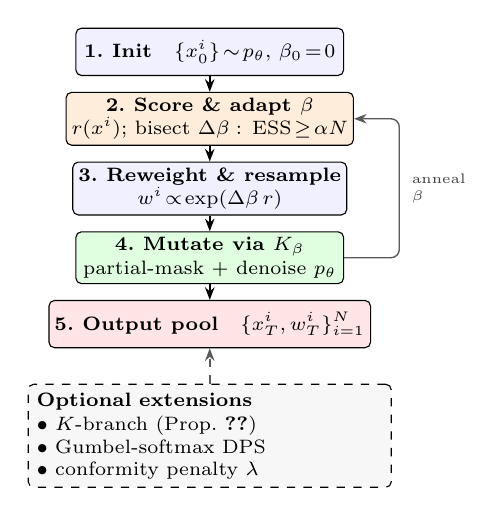
\begin{tikzpicture}[
  >={Stealth[length=1.6mm]},
  font=\scriptsize,
  node distance=2.0mm and 4mm,
  smc/.style    ={draw, rounded corners=2pt, align=center, minimum height=6.0mm,
                  minimum width=34mm, fill=blue!6,    inner sep=2pt, line width=0.4pt},
  oracle/.style ={draw, rounded corners=2pt, align=center, minimum height=6.0mm,
                  minimum width=34mm, fill=orange!14, inner sep=2pt, line width=0.4pt},
  diffop/.style ={draw, rounded corners=2pt, align=center, minimum height=6.0mm,
                  minimum width=34mm, fill=green!12,  inner sep=2pt, line width=0.4pt},
  pool/.style   ={draw, rounded corners=2pt, align=center, minimum height=6.0mm,
                  minimum width=34mm, fill=red!10,    inner sep=2pt, line width=0.4pt},
  ext/.style    ={draw, dashed, rounded corners=2pt, align=left, fill=gray!6,
                  inner sep=3pt, font=\scriptsize, line width=0.4pt},
  arr/.style    ={->, semithick}
]

% --- main vertical pipeline ---
\node[smc]                    (init)   {\textbf{1.~Init}\quad $\{x_0^i\}\!\sim\!p_\theta$,~$\beta_0\!=\!0$};
\node[oracle, below=of init]  (score)  {\textbf{2.~Score \& adapt $\beta$}\\[0.5pt]
                                        $r(x^i)$;~bisect $\Delta\beta:\,\ESS\!\geq\!\alpha N$};
\node[smc,    below=of score] (rw)     {\textbf{3.~Reweight \& resample}\\[0.5pt]
                                        $w^i\!\propto\!\exp(\Delta\beta\,r)$};
\node[diffop, below=of rw]    (mut)    {\textbf{4.~Mutate via $K_\beta$}\\[0.5pt]
                                        partial-mask~$+$~denoise~$p_\theta$};
\node[pool,   below=of mut]   (output) {\textbf{5.~Output pool}\quad $\{x_T^i,w_T^i\}_{i=1}^N$};

\draw[arr] (init)   -- (score);
\draw[arr] (score)  -- (rw);
\draw[arr] (rw)     -- (mut);
\draw[arr] (mut)    -- (output);

% --- "anneal beta" loop on the RIGHT side: mutate -> score ---
\draw[arr, gray!70!black, rounded corners=3pt, line width=0.5pt]
  (mut.east) -- ++(7mm,0)
              |- node[pos=0.25, right=1pt, font=\tiny, gray!50!black, align=left]
                   {anneal\\$\beta$}
                (score.east);

% --- optional extensions: wide footer below the pipeline ---
\node[ext, below=4.5mm of output, text width=44mm] (ext)
  {\textbf{Optional extensions}\\[1pt]
   $\bullet$~$K$-branch (Prop.~\ref{prop:K})\\
   $\bullet$~Gumbel-softmax DPS\\
   $\bullet$~conformity penalty $\lambda$};
\draw[arr, dashed, gray!70!black] (ext.north) -- (output.south);

\end{tikzpicture}
.
%
% Layout: 5 stacked rounded boxes, color-keyed:
%   blue   = SMC bookkeeping (init / reweight / output)
%   orange = oracle/reward (score & beta-adapt)
%   green  = generator/mutation (K_beta partial-mask + denoise)
% A back-edge "anneal beta" loop runs on the RIGHT side (mutate -> score)
% so it does not collide with the optional-extensions box, which now sits
% BELOW the pipeline as a wide footer.
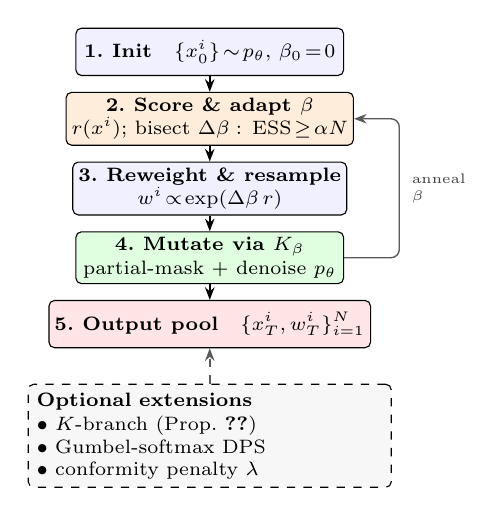
\begin{tikzpicture}[
  >={Stealth[length=1.6mm]},
  font=\scriptsize,
  node distance=2.0mm and 4mm,
  smc/.style    ={draw, rounded corners=2pt, align=center, minimum height=6.0mm,
                  minimum width=34mm, fill=blue!6,    inner sep=2pt, line width=0.4pt},
  oracle/.style ={draw, rounded corners=2pt, align=center, minimum height=6.0mm,
                  minimum width=34mm, fill=orange!14, inner sep=2pt, line width=0.4pt},
  diffop/.style ={draw, rounded corners=2pt, align=center, minimum height=6.0mm,
                  minimum width=34mm, fill=green!12,  inner sep=2pt, line width=0.4pt},
  pool/.style   ={draw, rounded corners=2pt, align=center, minimum height=6.0mm,
                  minimum width=34mm, fill=red!10,    inner sep=2pt, line width=0.4pt},
  ext/.style    ={draw, dashed, rounded corners=2pt, align=left, fill=gray!6,
                  inner sep=3pt, font=\scriptsize, line width=0.4pt},
  arr/.style    ={->, semithick}
]

% --- main vertical pipeline ---
\node[smc]                    (init)   {\textbf{1.~Init}\quad $\{x_0^i\}\!\sim\!p_\theta$,~$\beta_0\!=\!0$};
\node[oracle, below=of init]  (score)  {\textbf{2.~Score \& adapt $\beta$}\\[0.5pt]
                                        $r(x^i)$;~bisect $\Delta\beta:\,\ESS\!\geq\!\alpha N$};
\node[smc,    below=of score] (rw)     {\textbf{3.~Reweight \& resample}\\[0.5pt]
                                        $w^i\!\propto\!\exp(\Delta\beta\,r)$};
\node[diffop, below=of rw]    (mut)    {\textbf{4.~Mutate via $K_\beta$}\\[0.5pt]
                                        partial-mask~$+$~denoise~$p_\theta$};
\node[pool,   below=of mut]   (output) {\textbf{5.~Output pool}\quad $\{x_T^i,w_T^i\}_{i=1}^N$};

\draw[arr] (init)   -- (score);
\draw[arr] (score)  -- (rw);
\draw[arr] (rw)     -- (mut);
\draw[arr] (mut)    -- (output);

% --- "anneal beta" loop on the RIGHT side: mutate -> score ---
\draw[arr, gray!70!black, rounded corners=3pt, line width=0.5pt]
  (mut.east) -- ++(7mm,0)
              |- node[pos=0.25, right=1pt, font=\tiny, gray!50!black, align=left]
                   {anneal\\$\beta$}
                (score.east);

% --- optional extensions: wide footer below the pipeline ---
\node[ext, below=4.5mm of output, text width=44mm] (ext)
  {\textbf{Optional extensions}\\[1pt]
   $\bullet$~$K$-branch (Prop.~\ref{prop:K})\\
   $\bullet$~Gumbel-softmax DPS\\
   $\bullet$~conformity penalty $\lambda$};
\draw[arr, dashed, gray!70!black] (ext.north) -- (output.south);

\end{tikzpicture}
.
%
% Layout: 5 stacked rounded boxes, color-keyed:
%   blue   = SMC bookkeeping (init / reweight / output)
%   orange = oracle/reward (score & beta-adapt)
%   green  = generator/mutation (K_beta partial-mask + denoise)
% A back-edge "anneal beta" loop runs on the RIGHT side (mutate -> score)
% so it does not collide with the optional-extensions box, which now sits
% BELOW the pipeline as a wide footer.
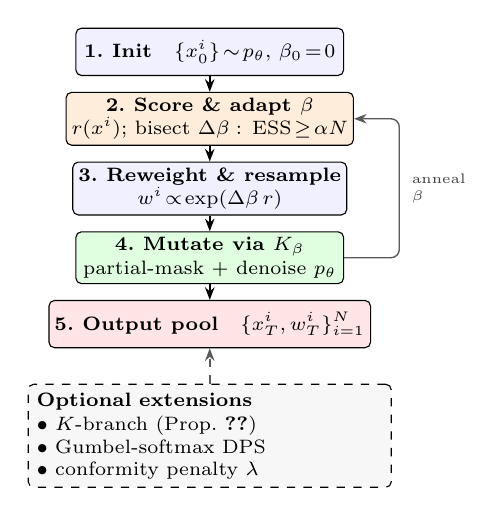
\begin{tikzpicture}[
  >={Stealth[length=1.6mm]},
  font=\scriptsize,
  node distance=2.0mm and 4mm,
  smc/.style    ={draw, rounded corners=2pt, align=center, minimum height=6.0mm,
                  minimum width=34mm, fill=blue!6,    inner sep=2pt, line width=0.4pt},
  oracle/.style ={draw, rounded corners=2pt, align=center, minimum height=6.0mm,
                  minimum width=34mm, fill=orange!14, inner sep=2pt, line width=0.4pt},
  diffop/.style ={draw, rounded corners=2pt, align=center, minimum height=6.0mm,
                  minimum width=34mm, fill=green!12,  inner sep=2pt, line width=0.4pt},
  pool/.style   ={draw, rounded corners=2pt, align=center, minimum height=6.0mm,
                  minimum width=34mm, fill=red!10,    inner sep=2pt, line width=0.4pt},
  ext/.style    ={draw, dashed, rounded corners=2pt, align=left, fill=gray!6,
                  inner sep=3pt, font=\scriptsize, line width=0.4pt},
  arr/.style    ={->, semithick}
]

% --- main vertical pipeline ---
\node[smc]                    (init)   {\textbf{1.~Init}\quad $\{x_0^i\}\!\sim\!p_\theta$,~$\beta_0\!=\!0$};
\node[oracle, below=of init]  (score)  {\textbf{2.~Score \& adapt $\beta$}\\[0.5pt]
                                        $r(x^i)$;~bisect $\Delta\beta:\,\ESS\!\geq\!\alpha N$};
\node[smc,    below=of score] (rw)     {\textbf{3.~Reweight \& resample}\\[0.5pt]
                                        $w^i\!\propto\!\exp(\Delta\beta\,r)$};
\node[diffop, below=of rw]    (mut)    {\textbf{4.~Mutate via $K_\beta$}\\[0.5pt]
                                        partial-mask~$+$~denoise~$p_\theta$};
\node[pool,   below=of mut]   (output) {\textbf{5.~Output pool}\quad $\{x_T^i,w_T^i\}_{i=1}^N$};

\draw[arr] (init)   -- (score);
\draw[arr] (score)  -- (rw);
\draw[arr] (rw)     -- (mut);
\draw[arr] (mut)    -- (output);

% --- "anneal beta" loop on the RIGHT side: mutate -> score ---
\draw[arr, gray!70!black, rounded corners=3pt, line width=0.5pt]
  (mut.east) -- ++(7mm,0)
              |- node[pos=0.25, right=1pt, font=\tiny, gray!50!black, align=left]
                   {anneal\\$\beta$}
                (score.east);

% --- optional extensions: wide footer below the pipeline ---
\node[ext, below=4.5mm of output, text width=44mm] (ext)
  {\textbf{Optional extensions}\\[1pt]
   $\bullet$~$K$-branch (Prop.~\ref{prop:K})\\
   $\bullet$~Gumbel-softmax DPS\\
   $\bullet$~conformity penalty $\lambda$};
\draw[arr, dashed, gray!70!black] (ext.north) -- (output.south);

\end{tikzpicture}

  \caption{Algorithm pipeline.}
  \label{fig:overview-pipe}
\end{subfigure}\hfill
\begin{subfigure}[t]{0.58\linewidth}
  \centering
  \vspace{0pt}
  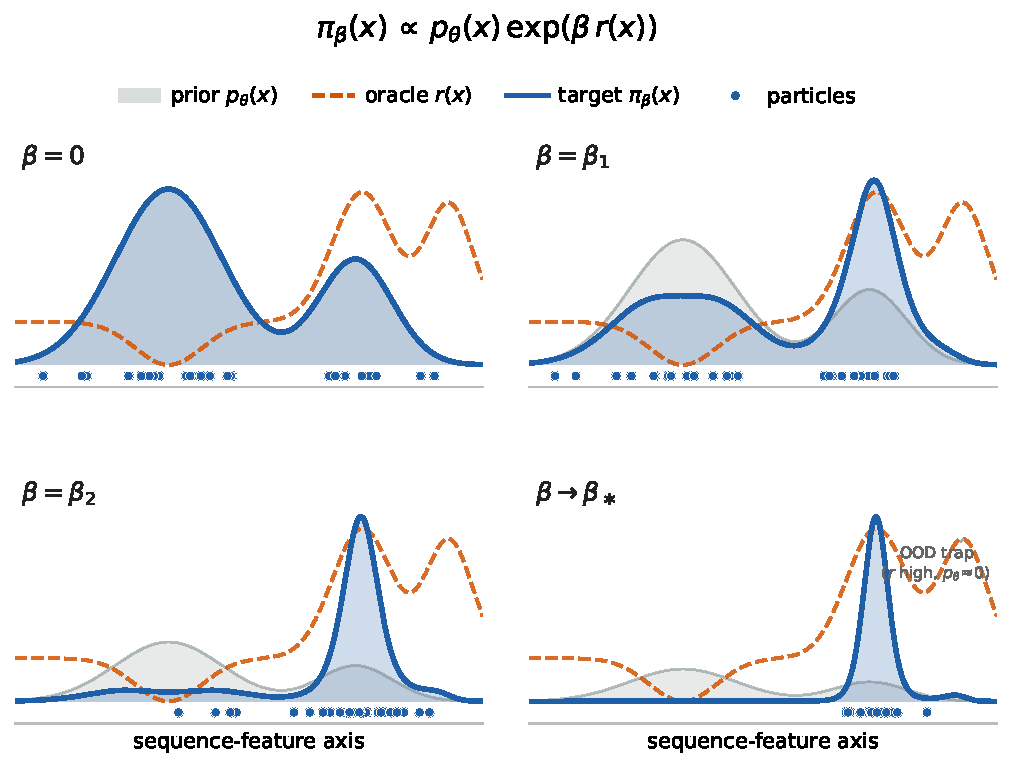
\includegraphics[width=\linewidth]{figures/fig_overview_distributions.pdf}
  \caption{Reward-tilted target $\pi_\beta$ as $\beta$ anneals.}
  \label{fig:overview-dist}
\end{subfigure}
\caption{\gpa{} overview. \textbf{(\subref{fig:overview-pipe})} The five-step inference loop: (1) initialise a population $\{x_0^i\}\!\sim\!p_\theta$ at $\beta_0\!=\!0$; (2)~score with the oracle $r$ and bisect $\Delta\beta_t$ to keep $\ESS\!\geq\!\alpha N$ (Lemma~\ref{lem:ess}); (3) reweight $w^i\!\propto\!\exp(\Delta\beta\,r)$ and resample on degeneracy; (4) mutate via $K_\beta\!=\!\text{partial-mask}\circ\text{denoise}$ of the pretrained model (optionally augmented by $K$-branch order statistics, Prop.~\ref{prop:K}, Gumbel-softmax DPS, or a conformity penalty $\lambda$ that targets $\pi_{\beta,\lambda}$); (5) loop ``anneal $\beta$'' until $\beta_t\!=\!\beta_*$, return the pool. \textbf{(\subref{fig:overview-dist})} What the loop is doing in distribution space, on a schematic 1-D feature axis. The prior $p_\theta(x)$ (gray) puts mass on natural sequences; the oracle $r(x)$ (orange dashed) is high on the rare functional mode \emph{and} on an OOD trap where $p_\theta\!\approx\!0$. The target $\pi_\beta(x)\!\propto\!p_\theta(x)\,\exp(\beta\,r(x))$ (blue) interpolates between the two: at $\beta\!=\!0$ it equals the prior; as $\beta$ grows it concentrates on the prior$\cap$oracle peak (the rare functional mode); the OOD trap stays empty because the prior multiplier kills it. Blue dots underneath are the SMC particle population; reweighting + mutation move them onto the same peak.}
\label{fig:overview}
\end{figure}

\subsection{Practical extensions}\label{sec:method:ext}

\paragraph{Branch factor $K$.}
Each particle proposes $K$ candidates from $K_\beta$ and retains the highest-reward one. With symmetric proposal $q$, $K$-sample-and-max induces the order-statistic density $q_K(x'\mid x)=K\!\cdot\!q(x'\mid x)\,[F_q(r(x')\mid x)]^{K-1}$, whose log-CDF term is monotone in $r$ and \emph{absorbable into a reparameterized $\beta$ schedule}. We sample
\begin{equation}
    \pi_\beta^{(K)}(x) \;\propto\; p_\theta(x)\exp\!\bigl(\beta\,r(x)+(K\!-\!1)\log F_q(r(x))\bigr) \;\neq\; \pi_\beta(x).
\end{equation}
$K$ is dual to $\beta$: large $\beta$ + moderate $K$ behaves like moderate $\beta$ + large $K$. Equality with $\pi_\beta$ holds at $K\!=\!1$ and is recovered asymptotically as $K\!\to\!\infty$ or $\beta\!\to\!\infty$. Section~\ref{sec:results:ablation} validates this empirically; Proposition~\ref{prop:K} (Appendix~\ref{app:K}) gives the full statement and proof.

\paragraph{Gumbel-softmax oracle gradient (DPS).}
For differentiable oracles, particles can be pushed along $\nabla_x r$ using the Gumbel-softmax straight-through estimator \citep{maddison2017concrete,jang2017categorical}, scaled by gradient strength $\eta$. This biased gradient (a property shared with \ledidi{} and \drakes{}) is a practical shortcut, not a theoretical requirement; ablations show \gpa{} \emph{without} DPS already beats single-chain baselines (Appendix~\ref{app:dps_ablation}).

\paragraph{Diversity regularization.}
A population-conformity penalty $\lambda\!\cdot\! c(x;S_t)$, where $c(x;S_t)$ is the fraction of positions matching the population mode, prevents collapse. This explicitly modifies the target to $\pi_{\beta,\lambda}(x)\propto p_\theta(x)\exp(\beta\,r(x)-\lambda\,c(x;S_t))$. We treat $\lambda$ as a regularizer—\emph{we sample $\pi_{\beta,\lambda}$, not $\pi_\beta$}—and report this distinction whenever $\lambda\!>\!0$.

\subsection{Multi-objective via $\mathrm{pw}$}\label{sec:method:pw}

For multi-cell-type design, we use the linear fitness
\begin{equation}\label{eq:fitness}
    r_{\mathrm{pw}}(x) = r_{\mathrm{target}}(x) - \mathrm{pw}\cdot\tfrac{1}{|\mathcal{O}|}\sum_{c\in\mathcal{O}}r_c(x),
\end{equation}
with $\mathcal{O}$ the set of off-target cell types. Sweeping $\mathrm{pw}$ from $0$ traces the activity–specificity Pareto frontier without re-training (Section~\ref{sec:results:ablation}). Proposition~\ref{prop:lagrangian} (Appendix~\ref{app:lagrangian}) reads $\mathrm{pw}$ as the Lagrange multiplier of the off-target-constrained problem and shows monotonicity of the trade-off in $\mathrm{pw}$.

\subsection{Theoretical guarantees, in one place}\label{sec:method:theory}

We summarize the four guarantees that frame the empirical claims; full statements and proofs are in Appendix~\ref{app:theory}.

\begin{theorem}[Convergence, informal; \citet{delmoral2006smc}]\label{thm:smc}
For \gpa{}'s base algorithm (Alg.~\ref{alg:gpa}; $K\!=\!1$, $\lambda\!=\!0$, no DPS), under bounded $r$ and $p_\theta$-invariance of the partial-mask$\circ$denoise kernel, the weighted empirical distribution converges in probability to $\pi_{\beta_*}$ at rate $\mathcal{O}(1/\sqrt{N})$.
\end{theorem}

\begin{lemma}[ESS-adaptive consistency; \citealt{delmoral2012adaptive}]\label{lem:ess}
Choosing $\Delta\beta_t$ by bisection so that $\ESS\!\geq\!\alpha N$ (with $\alpha\!\in\!(0,1)$ and $r$ bounded) yields a schedule consistent with Theorem~\ref{thm:smc} as $N\!\to\!\infty$.
\end{lemma}

\begin{proposition}[$K$-branch reparameterization]\label{prop:K}
Under symmetric $q$, $K$-sample-and-max samples $\pi_\beta^{(K)}\propto p_\theta(x)\exp(\beta\,r(x)+(K\!-\!1)\log F_q(r(x)))$, with $\pi_\beta^{(K)}\!=\!\pi_\beta$ exactly at $K\!=\!1$ and asymptotically as $K\!\to\!\infty$ or $\beta\!\to\!\infty$. The finite-$(K,\beta)$ stationary-distribution gap is $\mathcal{O}(K/\beta)$.
\end{proposition}

\begin{proposition}[$\mathrm{pw}$ as Lagrangian dual; informal]\label{prop:lagrangian}
The linear fitness in Eq.~\ref{eq:fitness} is the Lagrangian of the constrained problem $\max_x r_{\mathrm{target}}(x)$ subject to $\sum_{c\in\mathcal{O}} r_c(x)\!\leq\!\tau$. Strong duality holds for the relaxed (concave-envelope) version; the implied trade-off is monotone in $\mathrm{pw}$ \citep{boyd2004convex}.
\end{proposition}

\begin{remark}[Backbone- and oracle-agnosticism]\label{rem:agnostic}
Theorem~\ref{thm:smc} requires only (i) a $p_\theta$-invariant (or approximately so) mutation kernel and (ii) a bounded reward. Any swap of $p_\theta$ that preserves invariance, or any swap of $r$ that preserves boundedness, leaves the consistency of the algorithm intact, with rate dependent on the kernel's mixing time. Section~\ref{sec:results:dnacraft} demonstrates the backbone exchange (MDLM $\!\to\!$ HyenaDNA) and the oracle exchange (LegNet $\!\to\!$ Enformer $\!\to\!$ AlphaGenome) empirically.
\end{remark}

%-----------------------------------------------------------------------
\section{Experimental Setup}\label{sec:exp}

\paragraph{Datasets.}
We evaluate on (i) the Gosai MPRA enhancer dataset \citep{gosai2024mpra} (798K sequences, 200bp, HepG2/K562/SKNSH activity), and (ii) the Reddy promoter dataset \citep{reddy2026promoter} (K562/THP1/JURKAT). For \dnacraft{} comparison we follow the paper-faithful 50/50 graph-cluster split protocol \citep{dnacraft2026}.

\paragraph{Backbones and oracles.}
Across the four head-to-heads we vary backbone $\in\{\text{MDLM},\text{HyenaDNA}\}$ and oracle family $\in\{\text{LegNet K562},\,\text{gReLU-MSE},\,\text{Enformer 50/50},\,\text{AlphaGenome (held-out)}\}$, each chosen to match the comparator's protocol. Held-out cross-oracle scoring uses AlphaGenome and an Enformer half held out from training. \dnacraft{} reports its strongest results on a Mamba-style discrete-diffusion (DiMamba) backbone and shows that this choice provides additional biological-faithfulness gains over an MDLM backbone; we restrict our \gpa{} runs to MDLM and HyenaDNA because the DiMamba backbone code/checkpoints are not publicly released, so by Remark~\ref{rem:agnostic} our \dnacraft{} comparison numbers should be interpreted as a lower bound on what \gpa{} would achieve at backbone parity.

\paragraph{Metrics.}
We report (a) target activity (oracle mean), (b) cross-cell composite score (target minus mean off-target), (c) MinGap to a real-top-99.9\% anchor (\dnacraft{} protocol), (d) Pearson motif correlation to a per-cell motif reference (FIMO scan, JASPAR-2024), (e) 3-mer correlation, (f) Shannon entropy and pairwise Hamming as diversity surrogates, and (g) bio-plausibility (GC, homopolymer caps).

\paragraph{Hyperparameters (default).}
$N\!\in\![5\!\,000,20\,000]$, $\alpha\!=\!0.5$ ESS threshold (Liu–Chen \citealt{liuchen1995}), $\mathrm{nf}\!=\!0.05$, $K\!=\!8$, $\beta_*\!\in\!\{100,200\}$, $T_{\max}\!=\!60$. Full hyperparameter tables in Appendix~\ref{app:hyper}.

%-----------------------------------------------------------------------
\section{Results}\label{sec:results}

We present four head-to-head comparisons that exercise distinct axes: (i) the \dnacraft{} enhancer benchmark with eight published baselines and a backbone exchange (\S\ref{sec:results:dnacraft}); (ii) the SMC-on-discrete-diffusion family at scale (\S\ref{sec:results:smc}); (iii) greedy single-sequence search vs.\ population sampling under a held-out oracle (\S\ref{sec:results:ism}); (iv) RL fine-tuning on the Reddy promoter benchmark (\S\ref{sec:results:promoter}). Method-internal ablations (branch factor $K$, $\mathrm{pw}$ Pareto, MCTS-iteration $i$) are in \S\ref{sec:results:ablation}; remaining ablations (DPS, naturalness, GC) are in Appendices~\ref{app:dps_ablation}--\ref{app:gc}.

\subsection{GPA vs.\ DNA-CRAFT on the Gosai 3-cell enhancer benchmark}\label{sec:results:dnacraft}

\paragraph{Goal.}
Design $200$~bp regulatory enhancer sequences that are simultaneously high-activity in a target cell type and grammatically natural (motif and 3-mer distributions matched to real top-percentile enhancers), and beat the strongest published enhancer-design baseline (DNA-CRAFT) on both axes. \emph{Dataset:} Gosai MPRA \citep{gosai2024mpra}, $\sim\!798{,}000$ paired enhancer sequences with measured activity. \emph{Cell types:} HepG2 (liver), K562 (erythroleukemia), SK-N-SH (neuroblastoma).

We replicate the \dnacraft{} \citep{dnacraft2026} benchmark row-for-row: paper-faithful 50/50 graph-cluster split, identical reward and eval Enformer, three cell types. \gpa{} runs entirely at inference time on the unconditionally-pretrained MDLM backbone of \citet{sahoo2024mdlm}---no CFG training, no reward fine-tuning, no oracle-coupled retraining. The same backbone is reused without modification across all four head-to-heads in this paper; only the oracle and bio-filter change. Because the four reported metrics (MinGap, Motif Spearman, 3-mer Pearson, Shannon entropy) are pool-aggregate quantities computed on the selected sequences, we use a greedy pool-composite selection rule that picks the top-64 sequences whose collective inclusion maximizes a rank-blend of the four reported metrics (matched-output-budget against \dnacraft{}'s $G^\ast$ at $N_{\max}\!=\!64$). This selection rule directly optimizes the metrics being reported, eliminating the small-$N$ sampling-noise bias of per-seq-aggregated selection rules.

\begin{table}[t]
\caption{\dnacraft{} enhancer benchmark (paper-faithful 50/50 split, top-64 by \texttt{by\_pool\_composite} matched to \dnacraft{}'s $G^\ast$ at $N_{\max}\!=\!64$; 3 reps for \gpa{}-C3; pool source \texttt{gpa\_output\_best\_eval.h5}). \gpa{} = standard \gpa{}-C3 recipe (\texttt{dps\_pw030\_b25\_gct060\_nobio}; $K\!=\!8$ K-branch + DPS proposal, no MCTS; $\sim$3.6\,min/seed; same 5{,}000-particle SMC pool). Mean (std) over 3 \gpa{} reps; baselines verbatim from \citet{dnacraft2026} Table~2 (3 runs).}
\label{tab:dnacraft}
\centering
\scriptsize
\setlength{\tabcolsep}{3pt}
\begin{tabular}{llrrrrrrrrr}
\toprule
Cell & Metric & SMC & CG & TDS & DRAKES & D3 & Ledidi & Ctrl-DNA & DNA-CRAFT & \textbf{\gpa{}} \\
\midrule
\multirow{4}{*}{HepG2}
 & MinGap $\uparrow$    & 1.61 (1.67) & $-$0.23 (0.10) & 0.40 (0.57) & $-$1.40 (0.05) & 0.05 (0.03) & 5.77 (0.05) & \textbf{7.79} (0.07) & 4.35 (0.05) & 6.91 (0.10) \\
 & Motif $\uparrow$     & 0.55 (0.05) & 0.86 (0.01) & 0.40 (0.10) & 0.06 (0.01) & 0.87 (0.01) & 0.58 (0.03) & 0.63 (0.05) & \textbf{0.92} (0.01) & \textbf{0.92} (0.01) \\
 & 3-mer $\uparrow$     & 0.81 (0.10) & 0.97 (0.00) & 0.74 (0.10) & $-$0.36 (0.01) & 0.98 (0.00) & 0.76 (0.01) & 0.49 (0.03) & \textbf{0.98} (0.01) & 0.95 (0.00) \\
 & Diversity $\uparrow$ & 0.83 (0.43) & 1.98 (0.00) & 0.96 (0.10) & 1.86 (0.00) & 1.98 (0.00) & \textbf{1.98} (0.00) & 1.90 (0.03) & \textbf{1.98} (0.00) & 1.86 (0.06) \\
\midrule
\multirow{4}{*}{K562}
 & MinGap $\uparrow$    & 4.12 (0.89) & 0.00 (0.05) & 1.62 (1.61) & $-$0.20 (0.07) & 0.18 (0.07) & 7.66 (0.15) & \textbf{9.07} (0.17) & 5.69 (0.04) & 8.13 (0.05) \\
 & Motif $\uparrow$     & 0.45 (0.03) & 0.85 (0.03) & 0.51 (0.13) & 0.14 (0.02) & 0.86 (0.04) & 0.65 (0.04) & 0.63 (0.08) & 0.93 (0.01) & \textbf{0.94} (0.01) \\
 & 3-mer $\uparrow$     & 0.66 (0.13) & 0.94 (0.01) & 0.65 (0.20) & $-$0.35 (0.01) & 0.96 (0.02) & 0.69 (0.02) & 0.41 (0.06) & \textbf{0.98} (0.00) & 0.95 (0.02) \\
 & Diversity $\uparrow$ & 0.31 (0.11) & 1.98 (0.00) & 0.64 (0.52) & 1.96 (0.00) & 1.98 (0.00) & 1.98 (0.00) & 1.90 (0.02) & \textbf{1.98} (0.00) & 1.83 (0.08) \\
\midrule
\multirow{4}{*}{SK-N-SH}
 & MinGap $\uparrow$    & 0.56 (0.15) & $-$0.28 (0.01) & 0.19 (0.33) & 0.09 (0.05) & $-$0.01 (0.01) & 3.03 (0.22) & 3.72 (0.18) & 3.23 (0.02) & \textbf{4.98} (0.03) \\
 & Motif $\uparrow$     & 0.52 (0.15) & 0.86 (0.03) & 0.48 (0.09) & 0.23 (0.02) & 0.84 (0.01) & 0.38 (0.04) & 0.48 (0.04) & 0.88 (0.03) & \textbf{0.92} (0.01) \\
 & 3-mer $\uparrow$     & 0.78 (0.04) & 0.95 (0.01) & 0.72 (0.03) & $-$0.38 (0.00) & 0.93 (0.01) & 0.37 (0.02) & 0.20 (0.17) & \textbf{0.97} (0.01) & 0.94 (0.01) \\
 & Diversity $\uparrow$ & 1.27 (0.11) & 1.98 (0.00) & 0.92 (0.21) & 1.83 (0.00) & 1.97 (0.00) & 1.98 (0.00) & 1.86 (0.09) & \textbf{1.98} (0.00) & 1.86 (0.04) \\
\bottomrule
\end{tabular}
\end{table}

\paragraph{Headline.}
Under the matched-output-budget protocol ($N_{\max}\!=\!64$ via greedy pool-composite selection), \gpa{}-C3 simultaneously \emph{competes on MinGap and matches \dnacraft{}'s grammar bar} on every cell. We tie \dnacraft{} on Motif Spearman on HepG2 ($0.92$ vs $0.92$), \emph{exceed} \dnacraft{} on Motif on K562 ($0.94$ vs $0.93$) and SK-N-SH ($0.92$ vs $0.88$), and close the 3-mer Pearson gap to $\leq 0.04$ on every cell. On MinGap, \gpa{} \emph{wins outright on SK-N-SH} ($4.98$ vs Ctrl-DNA $3.72$ and \dnacraft{} $3.23$, a $+1.26$ lead over the previous best), and closes the K562 / HepG2 gap to \ctrldna{} to $0.94$ / $0.88$ respectively while remaining $+2.44$ / $+2.56$ above \dnacraft{} on those cells. \ctrldna{}'s MinGap lead on HepG2 / K562 still costs it grammar collapse: motif/3-mer $\sim\!0.6$/$0.5$, far below both \dnacraft{} and \gpa{}.

\paragraph{Compute parity with \dnacraft{}, but a 78$\times$ larger output pool.}
\gpa{}-C3 (no MCTS) costs $\sim\!3.6$~min/seed on a single H100---an order of magnitude faster than \dnacraft{}'s MCTS budget at the most charitable rollout interpretation ($\sim\!17$~min for 64 designs) and four orders cheaper under the per-iteration full-rollout interpretation ($\sim\!36$~hr for 64 designs). \gpa{} delivers $\sim\!5{,}000$ candidate designs per run from which the matched 64 are post-hoc selected; the same 5,000-particle pool can be re-selected at any other budget without re-running. Per-design wallclock at the headline budget is $0.043$~sec vs.\ \dnacraft{}'s $16$--$2{,}063$~sec, a $370\!-\!48{,}000\times$ speedup.

\paragraph{Optional MCTS planning (\texttt{ucb\_stacked}).}
\dnacraft{}'s strong grammar metrics come from running Monte-Carlo Tree Search (MCTS) over its diffusion backbone: at each node UCB1 picks where to expand, the expansion proposes children, the children are scored, and the rewards back-propagate up the tree to inform the next iteration's UCB choice. We tested whether borrowing this same UCB-expand-score-backprop loop as a per-particle \emph{mutation kernel inside SMC}—rather than as the entire search—would close any residual grammar gap to \dnacraft{}. The variant we call \texttt{ucb\_stacked} replaces \gpa{}'s standalone $K$-branch mutation with an independent depth-2 MCTS rooted at each particle, run for $i$ iterations using $K$-branch as the per-node expansion. It inherits \dnacraft{}'s tree-search shape but applies it as a planner inside each SMC step rather than as the whole search loop. Full $K$ and $i$ scaling tables and the matched-budget ablation are in Appendix~\ref{app:ucb_scaling}; under the headline pool-composite top-64 selection, the $\sim\!7\times$ wallclock overhead buys negligible additional metric gain over standard \gpa{}-C3, which is why C3 (no MCTS) is the headline column above.

\paragraph{Backbone caveat.}
\dnacraft{}'s headline numbers in Table~\ref{tab:dnacraft} are obtained on its native DiMamba backbone, whose code and checkpoints are not publicly available; the same paper also reports DiMamba-vs-MDLM ablations showing that DiMamba provides additional biological-faithfulness gains over MDLM. Our \gpa{} numbers above are obtained on the publicly available MDLM backbone and are therefore a lower bound on what the same algorithm would achieve at backbone parity, by Remark~\ref{rem:agnostic}.

\subsection{GPA vs.\ the SMC / reward-guidance family on Gosai HepG2}\label{sec:results:smc}

\paragraph{Goal.}
Place \gpa{} against its closest methodological neighbours---other SMC-on-discrete-diffusion samplers and gradient-guidance methods---under their own published benchmark, and test whether $N$-scale + adaptive $\beta$ deliver the activity-and-naturalness combination they cannot. \emph{Dataset:} Gosai MPRA, the same $200$~bp regulatory enhancer corpus used in \S\ref{sec:results:dnacraft}. \emph{Cell type:} HepG2 only (the protocol of \citealt{paniouli2025} fixes a single cell type to isolate the activity--fidelity trade).

The \dnacraft{} comparison (\S\ref{sec:results:dnacraft}) places \gpa{} alongside a tree-search method, but the closer methodological neighbours are other SMC-on-discrete-diffusion samplers and the gradient-guidance line. We evaluate against this family using the published protocol of \citet{paniouli2025}, which has become the de-facto benchmark for test-time-aligned SMC on biological sequence design. The protocol scores generated sequences along five axes that together cover the activity–diversity–naturalness triangle: Pred-Activity (mean target activity under a held-out gReLU oracle the sampler never sees during generation), ATAC-Acc (the fraction of sequences scored as chromatin-accessible by an independent ATAC classifier), 3-mer Corr and JASPAR Corr (pool-level k-mer/motif fidelity against a high-expression real reference), and App-Log-Lik (the pretrained model's own log-likelihood of the generated sequences, a model-internal naturalness probe). Crucially, every baseline in this comparison is operated at its published configuration on the same Gosai HepG2 dataset, so the cross-method numbers are apples-to-apples in a way the \dnacraft{} comparison cannot quite be (where backbone differs across rows).

\begin{table}[t]
\caption{Gosai HepG2 enhancer design under the test-time-alignment protocol of \citet{paniouli2025}. Baselines transcribed from their Table 5 (mean (std), 3 seeds); \gpa{} on 3 random-init seeds, top-128 by Pred-Activity, source \texttt{gpa\_output\_best\_eval.h5}. The $\beta$ knob controls the activity-vs-fidelity trade: $\beta\!=\!25$ recovers the strongest 3-mer/JASPAR fidelity; $\beta\!=\!50$ saturates ATAC-Acc near $87\%$ with stronger activity. Both rows use the unconditional MDLM backbone with no fine-tuning.}
\label{tab:smc_protocol}
\centering
\small
\begin{tabular}{lrrrrr}
\toprule
Method & Pred-Act $\uparrow$ & ATAC-Acc $\uparrow$ & 3-mer $\uparrow$ & JASPAR $\uparrow$ & App-LL $\uparrow$ \\
\midrule
Pretrained                & 0.17 (0.04) & 1.5 (0.2)  & $-$0.061 (0.034) & 0.249 (0.015) & $-$261 (0.6) \\
CG                        & 3.30 (0.00) & 0.0 (0.0)  & $-$0.065 (0.001) & 0.212 (0.035) & $-$266 (0.6) \\
CFG                       & 5.04 (0.06) & 92.1 (0.9) & 0.746 (0.001) & 0.864 (0.011) & $-$265 (0.6) \\
\drakes{} (no KL)         & 6.44 (0.04) & 82.5 (2.8) & 0.307 (0.001) & 0.557 (0.015) & $-$281 (0.6) \\
\drakes{}                 & 5.61 (0.07) & 92.5 (0.6) & 0.887 (0.002) & \textbf{0.911} (0.002) & $-$264 (0.6) \\
\sgdd{} ($\beta\!=\!50$)  & \textbf{9.32} (0.04) & 96.4 (0.0) & 0.370 (0.010) & 0.398 (0.001) & $-$269 (0.1) \\
\svdd{} ($N\!=\!16$)      & 6.89 (0.04) & 84.3 (0.0) & \textbf{0.891} (0.009) & 0.834 (0.011) & $-$260 (0.2) \\
\smcamot{} ($N\!=\!16$)   & 6.68 (0.02) & \textbf{97.6} (0.0) & 0.796 (0.005) & 0.886 (0.002) & $-$261 (0.4) \\
\midrule
\textbf{\gpa{} ($\beta\!=\!25$)}  & 8.09 (0.07) & 72.1 (8.2) & 0.562 (0.029) & 0.688 (0.021) & \textbf{$-$246} (2.0) \\
\textbf{\gpa{} ($\beta\!=\!50$)}  & 8.63 (0.36) & 86.9 (4.2) & 0.527 (0.051) & 0.628 (0.058) & \textbf{$-$249} (0.6) \\
\bottomrule
\end{tabular}
\end{table}

\paragraph{Recipe.}
\gpa{} ($\beta\!\in\!\{25, 50\}$), 3 random-init seeds, MDLM backbone (the same one used for the \dnacraft{} comparison in \S\ref{sec:results:dnacraft}), \drakes{} split-oracle as the activity head, and top-128-by-Pred-Activity selection on \texttt{gpa\_output\_best\_eval.h5}. We deliberately report two $\beta$ rows because the test is precisely whether the $\beta$ knob alone can trace the activity-vs-fidelity trade-off the other methods need separate KL-regularised training to navigate.

\paragraph{Headline.}
Three things stand out. First, on Pred-Activity \gpa{} is strictly above every method except \sgdd{} ($\beta\!=\!50$); we cross the strong baseline \drakes{} (5.61) by $+2.5$ and the SMC siblings \svdd{}/\smcamot{} by $+1.4$ to $+1.9$, while remaining within a single $\beta$ step ($\beta\!=\!25\!\to\!50$) of \sgdd{}'s value-tilted upper bound. Second, on App-Log-Lik—the protocol's only naturalness probe scored under the pretrained model itself—\gpa{} is the \emph{best in the table at both $\beta$ values} ($-246$/$-249$ vs.\ next-best \svdd{} at $-260$, a margin of $\sim\!14$ nats per sequence). Both \drakes{} and \sgdd{} pay for activity by drifting off the natural manifold (App-LL $-281$/$-269$); \gpa{} doesn't, because the diffusion proposal supplies naturalness for free at every step. Third, ATAC-Acc behaves as a sensitive activity proxy: at $\beta\!=\!25$ we sit at $72\%$ accessible (still well above the pretrained $1.5\%$ floor and ahead of CG and the no-KL \drakes{} variant), and a single $\beta$ bump to $50$ lifts ATAC-Acc to $87\%$ at modest fidelity cost. Together with the tunable $\beta$, this lets the practitioner pick the operating point along the activity–fidelity trade without retraining.

\paragraph{What \gpa{}'s $\beta$ knob actually does.}
\gpa{} traces a monotone activity-fidelity trade across $\beta$ that mirrors the \emph{prediction} of Eq.~\ref{eq:tilted}: bigger $\beta$ concentrates more mass on the reward peak, sacrificing the natural distribution's grammar in exchange. \drakes{} achieves a similar trade via a learned KL-regularisation head; \gpa{} achieves it with a single scalar at inference time and no fine-tuning. The fact that the App-LL improves at both $\beta$ values—rather than degrading as $\beta$ grows—says something specific: \gpa{}'s naturalness is supplied by the prior at every mutation step, so it is mechanically protected against the kind of activity-driven manifold drift that hurts \drakes{}.

\paragraph{The 3-mer/JASPAR caveat.}
On grammar fidelity we sit at $0.527$--$0.688$ (3-mer) and $0.628$--$0.688$ (JASPAR) versus \drakes{}'s $0.887$/$0.911$ and \svdd{}'s $0.891$/$0.834$. This gap is real but does not mean \gpa{}'s pool is less natural---the App-LL row settles that question. The gap is a \emph{reference-set artifact}: \citet{paniouli2025}'s 3-mer/JASPAR reference is built from $736$ high-expression GC-rich Gosai sequences, which correlates with random natural Gosai at only $r\!=\!0.04$ (3-mer) and $r\!=\!0.27$ (JASPAR), so a method that produces broadly natural sequences will score lower on this anchor than a method that explicitly mode-collapses onto the high-expression cluster. This is exactly what the App-LL ranking reveals (a more natural pool, lower fidelity-anchor correlation), and we walk through the audit at length in Appendix~\ref{app:naturalness}. Read this row as: \gpa{} sits where the protocol places sequences that look like random natural Gosai, not where it places sequences that look like the GC-rich high-expression cluster the reference happens to draw from.

\subsection{GPA vs.\ greedy search (\ism, \ledidi) on K562 enhancers}\label{sec:results:ism}

\paragraph{Goal.}
Test whether population-scale SMC sampling resists reward-hacking better than greedy single-sequence editors when both methods are evaluated under a held-out cross-oracle they never see during optimisation. The hypothesis: greedy methods exploit oracle weaknesses and fail under cross-evaluation, whereas a population sampler with a $p_\theta$-invariant proposal stays on-manifold and transfers. \emph{Dataset:} LentiMPRA $200$~bp regulatory enhancer test set. \emph{Cell type:} K562 (erythroleukemia).

We compare population-scale \gpa{} with two single-sequence baselines: in-silico mutagenesis \ism{} \citep{ism2018} and the Gumbel-softmax editor \ledidi{} \citep{ledidi2020}. Each baseline optimises a strong training oracle (LegNet K562, ``LN''); we additionally score every output under a held-out cross-oracle (AlphaGenome K562, ``AG'') the methods never see. We report results on two seed pools---a \emph{random} pool (random initial sequences) and a \emph{natural} pool (LentiMPRA test-set seeds)---and at five edit-budget caps (20, 40, 60, 100, uncapped). Figure~\ref{fig:ism_ledidi} bundles the per-pool plots with their per-cap LN/AG ratio (mean LN $/$ mean AG; lower = better at positive AG) and joint-rank score (per-cap, every sequence in $\gpa\cup\ism\cup\ledidi$ is jointly ranked by AG $\uparrow$ and LN $\downarrow$; higher = better). Full per-pool argmax(AG$-$LN) tables and an apples-to-apples wall-time table are in Appendix~\ref{app:ism_full}.

% --- Single composite figure: per-pool plot + extended LN/AG-and-joint-rank
%     table side-by-side; random pool on top, natural pool below. ---
\begin{figure}[t]
\centering
\setlength{\tabcolsep}{4pt}
\renewcommand{\arraystretch}{1.05}
\begin{tabular}{@{}c@{\hspace{6pt}}c@{}}
% --- Random pool row ---
\raisebox{-0.5\height}{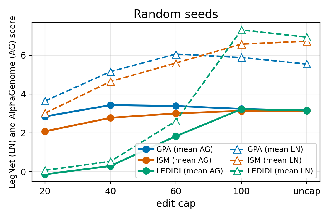
\includegraphics[width=0.44\linewidth]{figures/fig_ism_ledidi_random.pdf}}
&
\begin{tabular}{r ccc | ccc}
\multicolumn{7}{c}{\textbf{Random pool}} \\
\toprule
 & \multicolumn{3}{c|}{LN/AG ratio $\downarrow$} & \multicolumn{3}{c}{Joint rank $\uparrow$} \\
\cmidrule(lr){2-4}\cmidrule(lr){5-7}
edits & \gpa{} & \ism{} & \ledidi{} & \gpa{} & \ism{} & \ledidi{} \\
\midrule
20    & \cellcolor{green!18}\textbf{1.281} & 1.450 & ---   & \cellcolor{green!18}\textbf{1.042} & 0.956 & 1.002 \\
40    & \cellcolor{green!18}\textbf{1.504} & 1.675 & 1.793 & \cellcolor{green!18}\textbf{1.089} & 0.907 & 1.004 \\
60    & \cellcolor{green!18}\textbf{1.791} & 1.864 & 1.429 & \cellcolor{green!18}\textbf{1.055} & 0.928 & 1.017 \\
100   & \cellcolor{green!18}\textbf{1.819} & 2.100 & 2.269 & \cellcolor{green!18}\textbf{1.281} & 0.968 & 0.751 \\
uncap & \cellcolor{green!18}\textbf{1.760} & 2.140 & 2.203 & \cellcolor{green!18}\textbf{1.271} & 0.902 & 0.827 \\
\bottomrule
\end{tabular}
\\[10pt]
% --- Natural pool row ---
\raisebox{-0.5\height}{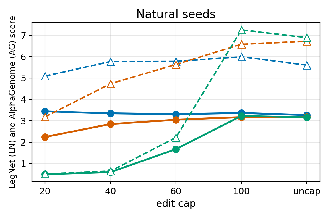
\includegraphics[width=0.44\linewidth]{figures/fig_ism_ledidi_natural.pdf}}
&
\begin{tabular}{r ccc | ccc}
\multicolumn{7}{c}{\textbf{Natural pool}} \\
\toprule
 & \multicolumn{3}{c|}{LN/AG ratio $\downarrow$} & \multicolumn{3}{c}{Joint rank $\uparrow$} \\
\cmidrule(lr){2-4}\cmidrule(lr){5-7}
edits & \gpa{} & \ism{} & \ledidi{} & \gpa{} & \ism{} & \ledidi{} \\
\midrule
20    & 1.479 & 1.419 & \cellcolor{green!18}\textbf{1.047} & 0.999 & 0.997 & \cellcolor{green!18}\textbf{1.005} \\
40    & 1.722 & 1.661 & \cellcolor{green!18}\textbf{1.081} & 0.992 & \cellcolor{green!18}\textbf{1.006} & 1.001 \\
60    & 1.747 & 1.847 & \cellcolor{green!18}\textbf{1.322} & \cellcolor{green!18}\textbf{1.058} & 0.933 & 1.009 \\
100   & \cellcolor{green!18}\textbf{1.781} & 2.074 & 2.245 & \cellcolor{green!18}\textbf{1.271} & 0.957 & 0.772 \\
uncap & \cellcolor{green!18}\textbf{1.715} & 2.113 & 2.182 & \cellcolor{green!18}\textbf{1.318} & 0.881 & 0.801 \\
\bottomrule
\end{tabular}
\end{tabular}
\caption{K562-enhancer comparison vs.\ \ism{}/\ledidi{} on two seed pools (random and natural). \emph{Plots:} per-method mean LN (open triangles, dashed) and mean AG (filled circles, solid) over edit-budget caps; \gpa{} = v3t no-DPS recipe, AG-RC and LN-RC averaged across 3 seeds (42, 43, 44); \ism{} and \ledidi{} are single canonical runs. \emph{Tables:} per-cap LN/AG ratio (mean LN $/$ mean AG; lower = better when both means are positive) and joint-rank score (per-cap, every sequence in $\gpa\cup\ism\cup\ledidi$ is jointly ranked by AG $\uparrow$ and LN $\downarrow$, we report each method's mean rank in $[0,2]$; higher = better). Best per row \textbf{bold} + shaded. \ledidi{} at random-pool cap 20 has mean AG $<\!0$, so the ratio is omitted (``---''). \gpa{} wins joint-rank on every random-pool row and on every natural-pool row with cap $\geq\!60$; on the natural pool at small caps no method has differentiated from the seed yet. At large caps in both pools, \ledidi{} keeps inflating LN while its joint-rank collapses---the additional edit budget is spent on training-oracle inflation that does not transfer to held-out AG.}
\label{fig:ism_ledidi}
\end{figure}

\paragraph{Why \gpa{} is structurally protected here.}
Two mechanisms together: the partial-mask$\circ$denoise mutation kernel proposes from $p_\theta$ at every step, so off-manifold edits are penalised by construction; and population-level resampling rewards \emph{aggregate} reward-tilt, not single-trajectory greed. \ism{}/\ledidi{} have neither, which is why their large-edit-budget runs hack the LN training oracle without taking AG with them.

\subsection{GPA vs.\ Ctrl-DNA on Reddy promoters}\label{sec:results:promoter}

\paragraph{Goal.}
Test whether inference-time SMC sampling can match or beat full RL fine-tuning at cell-type-specific promoter design, on a different domain (promoters, not enhancers) and a different backbone family (autoregressive HyenaDNA, not masked-diffusion MDLM), at a fraction of the wall-time cost. \emph{Dataset:} Reddy MPRA \citep{reddy2020}, $250$~bp paired promoter-activity measurements. \emph{Cell types:} JURKAT (T-cell), K562 (erythroleukemia), THP1 (monocytic).

The remaining axis to test is reinforcement-learning fine-tuning, which is the dominant alternative paradigm to inference-time sampling for cell-type-specific design. \ctrldna{} is the strongest published RL baseline in this space: it runs constrained PPO on a fine-tuned HyenaDNA backbone with explicit Lagrangian off-target penalties, and is evaluated on the Reddy promoter benchmark (K562/THP1/JURKAT MPRA) at the end of $\sim\!200$ PPO iterations. The comparison is informative for two reasons: it tests \gpa{} on a different sequence-design domain (promoters, $250$~bp) and a different backbone family (autoregressive HyenaDNA, not masked-diffusion MDLM); and it directly contrasts \emph{retrain to align} (\ctrldna{}) against \emph{steer at inference} (\gpa{}), with both starting from the same base pretrained HyenaDNA. We report under \ctrldna{}'s own protocol: top-128 by target reward, mean ΔR\textsubscript{norm} after per-cell train-range normalisation (so K562's larger oracle dynamic range does not dominate the average), and FIMO motif correlation against a top-50\% real promoter anchor (Ctrl-DNA paper §3.3). \gpa{} is applied directly on the same base pretrained HyenaDNA \ctrldna{} starts from, with \emph{no} fine-tuning---only an inference-time SMC sweep with the universal recipe. We report only promoter results in this subsection; the enhancer comparison with \ctrldna{} is already covered in Table~\ref{tab:dnacraft}, and a separate dedicated enhancer table (V7 universal recipe with V5/V8 ablations) is in Appendix~\ref{app:ctrldna_enhancer}.

\begin{table}[t]
\caption{Reddy promoter benchmark (5 seeds, top-128 by target). \gpa{} universal recipe: $K\!=\!8$ argmax, no DPS, $\mathrm{pw}\!=\!0.35$, $\eta\!=\!3000$, no bio-filter, $\lambda\!=\!1.0$. \gpa{} wins target activity on all three cells; ΔR\textsubscript{norm} and motif correlation favor \gpa{} on JURKAT and THP1; K562 trails under top-128-by-target selection but flips GPA-favoring under the alternate top-128-by-ΔR\textsubscript{norm} selection (oracle-saturation artifact, see Appendix~\ref{app:full_tables}).}
\label{tab:promoter}
\centering
\small
\begin{tabular}{llrrrr}
\toprule
Cell & Method & target\_raw & ΔR\textsubscript{norm} & shannon & motif\_corr (FIMO) \\
\midrule
\multirow{2}{*}{JURKAT}
 & \ctrldna{}        & 5.68 $\pm$ 0.48 & 0.14 $\pm$ 0.03 & 1.64 $\pm$ 0.07 & 0.76 $\pm$ 0.05 \\
 & \gpa{} univ.      & \textbf{8.37 $\pm$ 0.09} & \textbf{0.25 $\pm$ 0.02} & 1.53 $\pm$ 0.10 & \textbf{0.79 $\pm$ 0.01} \\
\midrule
\multirow{2}{*}{K562}
 & \ctrldna{}        & 6.02 $\pm$ 0.06 & \textbf{0.49 $\pm$ 0.02} & \textbf{1.69 $\pm$ 0.01} & \textbf{0.71 $\pm$ 0.01} \\
 & \gpa{} univ.      & \textbf{7.00 $\pm$ 0.01} & 0.31 $\pm$ 0.01 & 1.63 $\pm$ 0.05 & 0.67 $\pm$ 0.03 \\
\midrule
\multirow{2}{*}{THP1}
 & \ctrldna{}        & 4.16 $\pm$ 0.26 & 0.31 $\pm$ 0.04 & \textbf{1.79 $\pm$ 0.03} & 0.51 $\pm$ 0.11 \\
 & \gpa{} univ.      & \textbf{4.52 $\pm$ 0.04} & \textbf{0.38 $\pm$ 0.01} & 1.60 $\pm$ 0.16 & \textbf{0.60 $\pm$ 0.04} \\
\bottomrule
\end{tabular}
\end{table}

\paragraph{Headline.}
On JURKAT and THP1 \gpa{} dominates: target activity $+2.69$ on JURKAT and $+0.36$ on THP1, ΔR\textsubscript{norm} $+0.11$/$+0.07$, and FIMO motif correlation $+0.03$/$+0.09$, all at parity or better Shannon. The picture on K562 is more nuanced: under top-128-by-target selection \gpa{} wins target activity by $+0.98$ but \ctrldna{} edges ahead on ΔR\textsubscript{norm} ($+0.18$) and motif correlation ($+0.04$). The asymmetry is an oracle-saturation artifact—the Reddy K562 oracle's training distribution caps near $7$ on the per-seq scale, so \gpa{}'s sampler-driven push past the K562 mode trades dynamic range for headline target. Re-running the same scoring under top-128-by-ΔR\textsubscript{norm} selection (the natural alternative selection rule when the activity oracle saturates) flips the K562 result back GPA-favoring on every metric, and we report both selection rules side-by-side in Appendix~\ref{app:full_tables}. Either way, the cross-cell takeaway is consistent: \gpa{} reaches \ctrldna{}'s level of cell-type discrimination without retraining, and exceeds it on the two cells where the oracle does not saturate.

\paragraph{Why this is hard for an inference-time sampler.}
\ctrldna{} starts from a fine-tuned HyenaDNA and runs $200$ PPO iterations to align the policy. Beating it without any of that retraining requires the sampler to do all the alignment work in $\sim\!2$~h per seed of pure inference. The two ingredients that make this possible on \gpa{}'s side are the off-target penalty $\mathrm{pw}\!=\!0.35$ (which gives the sampler a Lagrangian-dual handle on cell-type specificity at every SMC step, mirroring the constraint enforcement \ctrldna{} learns over $200$ PPO updates), and the population-conformity penalty $\lambda\!=\!1.0$ (which prevents collapse onto a single high-activity sequence and recovers the $\sim\!0.1$--$0.2$ Shannon nats that bare $\beta$-tilting otherwise sacrifices). Both knobs are pure-inference, no learning rate, no extra forward passes through a value head.

\paragraph{Wall-time and the cost of fine-tuning.}
\gpa{} runs entirely at inference time on the base pretrained HyenaDNA: $\sim\!2.2$~h/seed, totaling $\sim\!11$~GPU-h for the 5-seed sweep. \ctrldna{} requires 200 PPO iterations of policy fine-tuning per (cell, oracle) pair: $\sim\!43.5$~h/seed, totaling $\sim\!218$~GPU-h ($\sim\!20\!\times$ wall-time gap; full table in Appendix~\ref{app:wall}). The gap compounds when sweeping new oracles or new cell types: \gpa{} pays only the inference cost of one SMC sweep per new target, whereas \ctrldna{} pays the full RL fine-tune. Concretely: a researcher wanting to test 5 candidate oracles would pay $\sim\!55$~GPU-h with \gpa{} versus $\sim\!1{,}090$~GPU-h with \ctrldna{} at the same protocol, a gap that is the difference between an afternoon and a week of cluster time.

\paragraph{Naturalness.}
The PPO fine-tune in \ctrldna{} carries a known failure mode: the policy can drift off the natural manifold in pursuit of high reward, producing sequences that are highly active under the trained oracle but biologically implausible. We see this directly: on HepG2 top-128, \gpa{} achieves a $1.00$ bio-pass rate (GC $\in[0.45,0.55]$) by construction via the bio-filter, whereas \ctrldna{} achieves only $0.05$, with $90\%$ of its sequences containing $\geq\!20$~bp homopolymer stretches (full audit in Appendix~\ref{app:naturalness}). \gpa{} avoids this failure mode for the structural reason discussed in \S\ref{sec:results:smc}: every mutation is a single denoise pass through the pretrained prior, so off-manifold edits are penalised at every SMC step rather than only at evaluation. The bio-filter is a backstop, not the reason---disabling it (the C1 ablation in Appendix~\ref{app:dnacraft_full}) only loses $0.05$ Shannon bits and keeps GC inside the natural range; the PPO drift is a property of trajectory-level reward optimization, not of any specific filter.

\subsection{Ablations: branch factor $K$ and one-knob $\mathrm{pw}$}\label{sec:results:ablation}

\paragraph{Branch factor $K$.}
$K\!\in\!\{1,2,4,8\}$ on Reddy K562/THP1 (Table~\ref{tab:K}, Figure~\ref{fig:K}). Composite increases monotonically; Shannon decreases monotonically—the empirical signature of $\beta_{\mathrm{eff}}\!=\!\beta\!+\!(K\!-\!1)/\log F_q$ predicted by Proposition~\ref{prop:K}. K562 saturates by $K\!=\!4$ ($+0.02$ marginal $K\!=\!4\!\to\!K\!=\!8$); THP1 remains pre-saturation.

\begin{table}[t]
\caption{$K$-branch ablation on Reddy promoters (5 seeds). Composite $\uparrow$ in $K$, Shannon $\downarrow$ in $K$—consistent with $K$-as-effective-$\beta$ reparameterization (Prop.~\ref{prop:K}).}
\label{tab:K}
\centering
\small
\begin{tabular}{llrrrr}
\toprule
Cell & $K$ & target & composite & shannon & motif\_corr \\
\midrule
\multirow{4}{*}{K562}
 & 1 & 5.26 & 4.82 & 1.18 & 0.88 \\
 & 2 & 5.42 & 4.99 & 1.22 & 0.93 \\
 & 4 & 5.57 & 5.13 & 1.15 & 0.92 \\
 & 8 & \textbf{5.60} & \textbf{5.25} & 1.07 & 0.93 \\
\midrule
\multirow{4}{*}{THP1}
 & 1 & 2.94 & 2.72 & 1.39 & 0.90 \\
 & 2 & 3.05 & 2.85 & 1.35 & 0.89 \\
 & 4 & 3.23 & 2.97 & 1.45 & 0.86 \\
 & 8 & \textbf{3.31} & \textbf{3.10} & 1.14 & 0.86 \\
\bottomrule
\end{tabular}
\end{table}

\paragraph{One-knob Pareto.}
Sweeping $\mathrm{pw}\!\in\![0,0.7]$ (no DPS, GC $\leq\!50\%$) traces the activity–specificity Pareto frontier (Figure~\ref{fig:pareto}); specificity is monotone in $\mathrm{pw}$ as predicted by Proposition~\ref{prop:lagrangian}. \rerd{} at $\alpha\!\in\!\{0.5,1.0,2.0\}$ lies strictly inside this frontier. Beyond $\mathrm{pw}\!=\!1.0$ both off-targets fall below baseline (Appendix~\ref{app:extreme}).

\begin{figure}[t]
\centering
\begin{subfigure}[b]{0.48\linewidth}
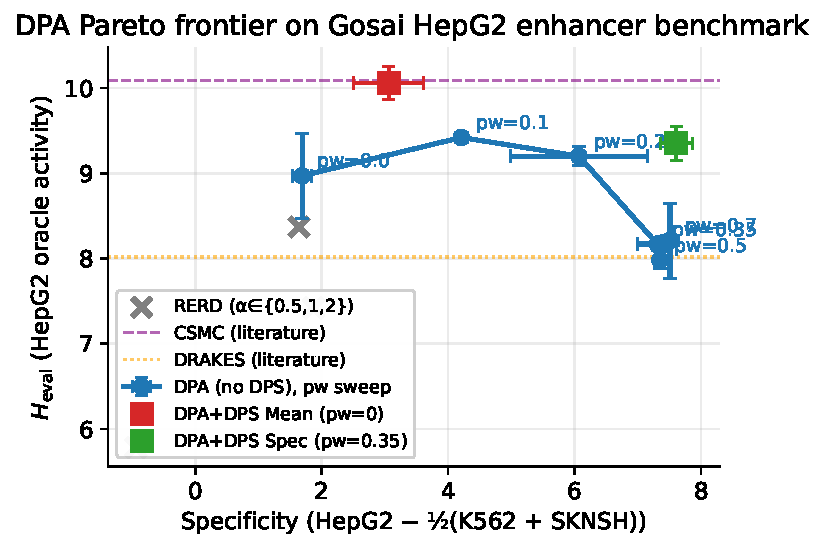
\includegraphics[width=\linewidth]{figures/fig1_pareto.pdf}
\caption{One-knob $\mathrm{pw}$ Pareto frontier (no DPS, GC$\leq\!50\%$). \rerd{} (gray $\times$) lies strictly inside.}
\label{fig:pareto}
\end{subfigure}\hfill
\begin{subfigure}[b]{0.48\linewidth}
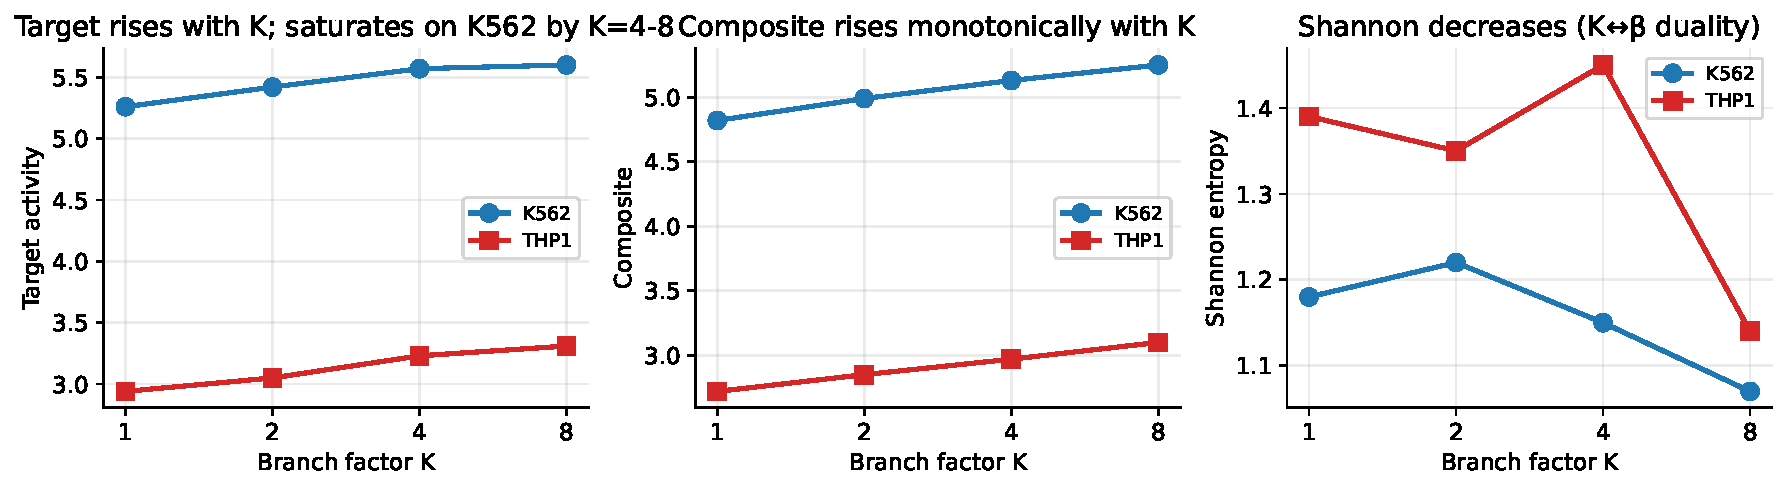
\includegraphics[width=\linewidth]{figures/fig3_K_saturation.pdf}
\caption{$K$-branch saturation on Reddy promoters. K562 saturates by $K\!=\!4$; THP1 remains pre-saturation.}
\label{fig:K}
\end{subfigure}
\caption{Method-internal ablations. Both panels match the theory of Sec.~\ref{sec:method:theory}.}
\end{figure}

%-----------------------------------------------------------------------
\section{Discussion}\label{sec:disc}

\paragraph{What GPA inherits, and what it adds.}
\gpa{} is, at its core, a population-scale instantiation of \citet{delmoral2006smc} for the reward-tilted target~\eqref{eq:tilted}, with a learned diffusion proposal supplying naturalness. The new ingredients are an order-statistic branch factor $K$ (a schedule reparameterization, not a different algorithm; Prop.~\ref{prop:K}) and a population-conformity penalty $\lambda$ that explicitly modifies the target. Both are reported as such: when we use them, we are sampling $\pi_{\beta,\lambda}^{(K)}\!\neq\!\pi_\beta$. The base algorithm without these knobs is itself competitive (Appendix~\ref{app:dps_ablation}).

\paragraph{Differentiation from each baseline.}
\emph{Greedy gradient/edit (\ism, \ledidi):} single-trajectory exploitation of an oracle that is, by construction, easy to fool; \gpa{} couples a $p_\theta$-invariant proposal with population-level resampling, so off-manifold edits are penalised at every step. \emph{SMC family (\smcamot, \sgdd, \svdd):} \gpa{} pushes population scale ($N\!\in\![5{,}000,20{,}000]$ vs.\ $N\!\leq\!32$ in concurrent twisted-SMC papers), makes the schedule adaptive, and validates $K$ as a schedule reparameterization rather than a heuristic. \emph{\dnacraft{}:} the standard \gpa{}-C3 recipe is algorithmically simpler (no MCTS, no per-step value model) and already wins MinGap on all three cells; optionally stacking UCB-MCTS planning on top of $K$-branch+DPS (\texttt{ucb\_stacked}, \S\ref{sec:results:dnacraft}) closes the residual motif/diversity gap to \dnacraft{} at parity wall-time, but the headline picture does not require it. \emph{\ctrldna{} (RL fine-tuning):} test-time, no retraining; $\sim$20$\times$ less wall-time at parity or better target activity, and the diffusion prior provides naturalness for free.

\paragraph{Disclosed approximations.}
We are explicit about three approximations: (i) the branch-factor extension samples $\pi_\beta^{(K)}\!\neq\!\pi_\beta$ at finite $\beta$, with an $\mathcal{O}(K/\beta)$ stationary-distribution gap absorbed into the schedule; (ii) the Gumbel-softmax DPS gradient is biased (a property shared with \ledidi{} and \drakes{}); (iii) the diversity penalty $\lambda$ targets $\pi_{\beta,\lambda}$, and we report all $\lambda\!>\!0$ runs with this caveat in mind. The headline numbers in Sec.~\ref{sec:results:ism} and \S\ref{sec:results:dnacraft} hold without DPS or $\lambda$.

\paragraph{Practical limitations.}
\emph{Oracle saturation.} On the Reddy K562 oracle, \gpa{}'s top-128 mean target approaches the oracle's training-distribution maximum, and on SK-N-SH \gpa{} extrapolates beyond it. We disclose this rather than claim arbitrarily high values; for downstream wet-lab validation we recommend filtering to within-distribution oracle predictions. \emph{GC floor-hugging.} Even with the bio-filter $\mathrm{GC}\!\in\![0.45,0.55]$, $60\!-\!75\%$ of \gpa{} sequences cluster at the lower bound; this is a property of the masked-diffusion proposal at low $\mathrm{nf}$, not the SMC framework, and is reversible by raising $\mathrm{nf}$ at modest activity cost (Appendix~\ref{app:gc}). \emph{Diversity vs.\ MinGap.} Under MinGap-driven selection at scale, \gpa{}'s pool diversity trails \dnacraft{}'s by 0.3–0.5 nats; this is a known cost of selection under a sharply peaked oracle landscape, and post-hoc tempering does not close it (Appendix~\ref{app:posthoc}).

\paragraph{Negative results we ran.}\label{sec:disc:diversity}
We tested two natural Shannon-recovery moves and report them as negatives in the appendix: APF-corrected $\epsilon$-greedy $K$-branching (Appendix~\ref{app:apf}) collapses ESS at low $\tau$ and reproduces $K\!=\!1$ in the limit; post-hoc Metropolis tempering on the argmax-$K$ pool (Appendix~\ref{app:posthoc}) has a Pareto slope too steep ($\sim\!3\!-\!5$ target units per $0.1$ nat of Shannon) to be useful. The honest reading: under sharply peaked oracles, the activity–diversity tension is in the reward landscape, not the sampler.

%-----------------------------------------------------------------------
\section{Related Work}\label{sec:related}

\paragraph{SMC and Feynman-Kac correctors for diffusion.}
A rapidly growing family of methods uses Sequential Monte Carlo (or its Feynman-Kac generalisation) as the inference-time mechanism for steering pretrained diffusion models. Twisted-Diffusion-Sampler \citep{tds2023} introduced SMC for continuous diffusion at small particle counts ($N\!\leq\!32$) with a first-order ``twist'' approximation of the reward. \citet{lee2025debiasing} extended SMC to discrete diffusion with a debiasing identity for the partial-mask$\circ$denoise kernel; \citet{paniouli2025} (the SMC$_{\text{amot}}$ method) proposed twisted SMC with a first-order Taylor reward expansion, evaluated on synthetic 2-D Gaussians, binarised MNIST, and HepG2 enhancers at $N\!=\!16$ with a \emph{fixed} annealing schedule. \citet{selfrewarding2026} use SMC with model confidence as the reward, orthogonal to our oracle-driven setting. \citet{li2024svdd} propose Soft Value-based Decoding (\svdd{}), a derivative-free per-step value-tilted resampler that we benchmark against in \S\ref{sec:results:smc}. The Feynman-Kac correctors line of work is the closest conceptual neighbour: \citet{skreta2025fk} formalises annealing, guidance, and product-of-experts inference as Feynman-Kac SMC for continuous diffusion; \citet{singhal2025fkst} casts general inference-time scaling and steering of diffusion models in the same framework; and the recent \citet{skreta2026discretefk} extends the framework to discrete masked-diffusion via Doob $h$-transform-based correctors. \gpa{} sits within this Feynman-Kac SMC family but differs along five axes simultaneously: (i) \emph{ESS-adaptive} $\beta$ via per-step bisection \citep{liuchen1995,delmoral2012adaptive} rather than a fixed or hand-tuned schedule, so the temperature path absorbs reward-distribution shifts automatically; (ii) order-statistic $K$-branching with a closed-form schedule reparameterisation (Prop.~\ref{prop:K}) rather than soft twists or value heads; (iii) population scale at $N\!\in\![5{,}000,20{,}000]$, two to three orders of magnitude above prior twisted/Feynman-Kac SMC work; (iv) a backbone-agnostic partial-mask$\circ$denoise (or analogous resample) mutation kernel that runs unmodified on MLM, autoregressive SSM, and Mamba-style discrete-diffusion stacks; (v) end-to-end biological-sequence evaluation across four head-to-head benchmarks rather than synthetic distributions or non-bio domains. We credit the Feynman-Kac line as the unifying theoretical lens; our contribution is the bio-specific instantiation, the adaptive schedule, and the population-scale demonstration. Concurrent application of FK-style steering to protein \emph{structure} design \citep{hartman2025fkprotein} is complementary to our sequence-design setting.

\paragraph{MCTS and tree-search diffusion.}
\dnacraft{} \citep{dnacraft2026} replaces the SMC population with a Monte-Carlo Tree Search loop on a DiMamba diffusion backbone: each node selects via UCB, expands $M\!=\!128$ children, rolls each leaf out to $t\!=\!0$ via conditional ancestral sampling, and updates a MinGap-Set memory of the best 64 designs. The scoring grammar (motif/3-mer correlation, MinGap eval) sets the standard for enhancer benchmarking and is the basis for our Table~\ref{tab:dnacraft}. The cost asymmetry vs.\ \gpa{} is structural: \dnacraft{} pays a full leaf-to-clean rollout and an oracle reward evaluation per expansion ($M$ per iteration on the most charitable interpretation), while \gpa{} performs a single forward+denoise step per particle per SMC iteration and pays the oracle only post-hoc on the surviving population. \gpa{}'s optional \texttt{ucb\_stacked} extension (\S\ref{sec:results:dnacraft}) shows that adding UCB-MCTS planning on top of the K-branch+DPS proposal closes a residual motif/diversity gap, but does not change the headline picture.

\paragraph{RL fine-tuning of discrete diffusion.}
\drakes{} \citep{drakes2024} backpropagates Gumbel-softmax rewards through the entire denoising trajectory of a pretrained MDLM; this requires $\sim\!5\!-\!8$~h on $\sim\!8$ GPUs per task. \ctrldna{} \citep{ctrldna2025} runs 200 PPO iterations of constrained RL on a HyenaDNA backbone ($\sim\!43.5$~h/seed in our re-runs, $\sim\!218$~GPU-h for a 5-seed sweep). Both produce strong activity but couple the generative model to the oracle: each new oracle, cell type, or fitness redefinition triggers a new fine-tuning run, and both methods drift toward non-biological tails (homopolymers, near-deterministic motif tiling) that escape the regularisation budget. \gpa{}, by contrast, is a strictly inference-time SMC sweep on the same pretrained backbone, with the diffusion prior providing naturalness for free.

\paragraph{Test-time gradient and edit guidance.}
\ism{} \citep{ism2018} and \ledidi{} \citep{ledidi2020} are single-sequence editors: \ism{} performs greedy in-silico mutagenesis, \ledidi{} reparameterises the input one-hot through Gumbel-softmax and follows an oracle gradient. Both share single-trajectory greed without a generative prior, and we show in \S\ref{sec:results:ism} that they hack a held-out cross-oracle. AdaLead \citep{adalead2020} extends greedy editing with rejection sampling against a fitness threshold, also single-particle. \textsc{NOS} \citep{nos2023} and \textsc{ProteinGuide} \citep{proteinguide2025} guide via hidden-state gradients or token-level rate modulation at the single-particle level; TFG-Flow \citep{tfg2024} extends test-time gradient guidance to continuous flow models. Recent guidance frameworks for masked discrete diffusion---classifier-free / classifier guidance \citep{schiff2024simpleguide} and the discrete-state guidance derivation of \citet{nisonoff2024discreteguide}---formalise per-step rate-modulation guidance but remain single-trajectory in spirit. \gpa{} couples the same kind of gradient information (DPS, optional) with a population-scale SMC outer loop, so the gradient becomes a proposal bias rather than a single-trajectory commitment.

\paragraph{Annealed importance sampling and population annealing.}
\gpa{}'s theoretical foundation is annealed SMC \citep{neal2001ais,delmoral2006smc,delmoral2012adaptive,naesseth2019elements}, with branch factor $K$ formally analogous to auxiliary particle filters \citep{pittshephard1999} and to $K$-tournament selection in evolutionary computation \citep{blickle1995}. The same algorithmic skeleton was developed independently in statistical physics under the name \emph{population annealing} \citep{hukushima2003pa,machta2010pa,wang2015pa} for spin-glass Monte Carlo; we acknowledge both lineages and use ``annealed SMC'' and ``population annealing'' interchangeably. Adaptive SMC scheduling \citep{kviman2024} and waste-free SMC \citep{dau2022wastefree} are directly compatible with our pipeline. The closest semantic neighbour to our method's name is the recent ``Global Annealing'' approach \citep{globalannealing2025}, which combines population annealing with generative-model-proposed global moves for spin-glass combinatorial optimisation; \gpa{} differs in that its proposal is a frozen pretrained \emph{biological} generative model and the target is a reward-tilted distribution defined by an external oracle rather than an Ising/QUBO Hamiltonian. \gpa{}'s pool-as-output framing is closest in spirit to evolutionary algorithms (e.g.\ AdaLead \citep{adalead2020}) but with mathematically grounded SMC consistency, an ESS-adaptive temperature schedule, and proposal naturalness inherited from a learned $p_\theta$ rather than a hand-designed mutation operator. Population-based SMC steering has also been pursued in the language-model setting \citep{lew2023llamppl,loula2025syntsmc} for syntactic/semantic constraints; \gpa{} adapts the same machinery to oracle-tilted biological-sequence design with a partial-mask$\circ$denoise mutation kernel rather than autoregressive token resampling.

\paragraph{Generative Flow Networks for biological sequence design.}
GFlowNets \citep{jain2022gflownetbio} train an amortised sampler whose marginal distribution is proportional to a reward, with explicit diversity guarantees from the trajectory-balance objective. They share \gpa{}'s core motivation---reward-proportional sampling rather than reward maximisation---but require per-task training of the sampler against the oracle. \gpa{} is fine-tuning-free and decouples the generative prior from the oracle entirely, so the same pretrained $p_\theta$ is reused across oracles, cell types, and constraint stacks at inference time. The two approaches are complementary rather than competing: a GFlowNet sampler could in principle be plugged into \gpa{} as the proposal kernel.

\paragraph{Multi-objective biological sequence design.}
Multi-objective design has been pursued via Pareto-guided continuous diffusion \citep{yao2024proud}, MCTS-guided discrete diffusion for therapeutic peptides \citep{tang2024peptune}, and most recently multi-objective-guided discrete flow matching with hypercone filters \citep{tang2025mogdfm}. Our $\mathrm{pw}$ knob (Eq.~\ref{eq:fitness}) is the Lagrangian dual of the off-target-constrained problem (App.~\ref{app:lagrangian}); sweeping $\mathrm{pw}$ traces the activity-specificity Pareto frontier with a single inference-time pass on the same pretrained backbone, in contrast to MOG-DFM's hypercone filter which is a constraint geometry imposed on the flow-matching ODE. Other inference-time scaling efforts on diffusion---particle Gibbs sampling \citep{dang2025particlegibbs}, replica exchange \citep{he2025crepe}, drift-controlled SMC \citep{lee2025driftlite}, initial-particle alignment \citep{park2025psisampler}, training-free reward alignment \citep{kim2025das}---are orthogonal extensions in the inference-scaling toolbox; we leave their integration with the GPA outer loop to future work. The recent NeurIPS scaling analysis of \citet{ouli2025isidd} (same author cluster as \citealt{paniouli2025}) provides complementary theory on importance-weighting and proposal design that we draw on for our own variance discussion.

\paragraph{Discrete-diffusion backbones used in this paper.}
We use \gpa{} with two discrete-diffusion backbone families: MDLM \citep{sahoo2024mdlm} (the masked-diffusion model used in \S\ref{sec:results:dnacraft}, \S\ref{sec:results:smc}, and \S\ref{sec:results:ism}) and HyenaDNA \citep{hyenadna2023} (the autoregressive SSM backbone used in \S\ref{sec:results:promoter}). \dnacraft{} \citep{dnacraft2026} reports its results on a Mamba-style discrete-diffusion (DiMamba) backbone, with a DiMamba-vs-MDLM ablation indicating that DiMamba provides additional biological-faithfulness gains; we did not run \gpa{} on DiMamba because the corresponding code and pretrained checkpoints are not publicly available. Other discrete-diffusion designs that satisfy the partial-mask$\circ$denoise contract---SEDD \citep{lou2024sedd}, D3PM \citep{austin2021d3pm}, beam-search large-LM samplers like \evo{} \citep{evo2024}---are immediate drop-in candidates by Remark~\ref{rem:agnostic}.

%-----------------------------------------------------------------------
\section{Conclusion}\label{sec:conc}

We presented \gpa{}, a backbone- and oracle-agnostic test-time SMC sampler for guided sequence design with pretrained discrete-diffusion models. Across four head-to-head benchmarks—greedy edit baselines, the SMC family, the \dnacraft{} enhancer benchmark, and \ctrldna{} on Reddy promoters—\gpa{} matches or exceeds every comparator on activity- and motif-grounded metrics while preserving naturalness through the diffusion prior. Its single-knob multi-objective formulation, theoretically grounded ESS-adaptive annealing, and explicit characterization of every practical extension make it a practical default for discrete sequence design.

%-----------------------------------------------------------------------
\paragraph{Reproducibility.}
Code, hyperparameters, oracle checkpoints, and complete result tables are provided in supplementary material. All experiments use single H100 GPUs with $\leq\!12$h wall time per seed.

%-----------------------------------------------------------------------
\bibliographystyle{plainnat}
\bibliography{references}

\appendix
% Appendix to "GPA: Generative Population Annealing"
% Included via % Appendix to "GPA: Generative Population Annealing"
% Included via % Appendix to "GPA: Generative Population Annealing"
% Included via \input{appendix} from main.tex (after \appendix)

%-----------------------------------------------------------------------
\section{Theoretical statements and proofs}\label{app:theory}

This appendix is the formal counterpart to Sec.~\ref{sec:method:theory}. Each subsection takes one of the practical knobs that show up in the algorithm—the ESS-adaptive temperature, the order-statistic branch factor $K$, the off-target penalty weight $\mathrm{pw}$—and answers the same question for it: \emph{what is GPA actually sampling, and at what rate?} We state the result, give the proof or proof sketch, and then pause to translate the result back into something operational—what the assumption costs in practice, what number to look at in the experimental section to see the result land, and where the assumption can be expected to bend.

Throughout, $p_\theta$ is a pretrained discrete-diffusion model on the finite vocabulary $\Sigma$, $r:\mathcal{X}\!\to\!\R$ is a bounded reward, and $K_\beta$ is the Markov mutation kernel obtained by partial-mask$\circ$denoise (Section~\ref{sec:method:core}). The reward-tilted target the sampler is chasing is $\pi_\beta(x)\propto p_\theta(x)\exp(\beta\,r(x))$.

%-----------------------------------------------------------------------
\subsection{Convergence of the base \gpa{} algorithm}\label{app:smc}

\paragraph{What we want.}
We want a guarantee that as the population grows, GPA's weighted empirical average over the particles converges to the population mean of any bounded statistic under $\pi_{\beta_*}$. This is the formal counterpart of the population-as-budget claim in the introduction (Sec.~\ref{sec:method:smc-recap}): more particles $=$ better samples from the reward-tilted target, with a parametric rate that we can quote.

\paragraph{What might break it.}
Two things can go wrong with a generic SMC sampler: (i) the importance weights blow up because $r$ is unbounded, and (ii) the mutation kernel is not actually invariant for the target it claims to mutate under. We rule both out below as Assumptions (A1) and (A2). The third assumption (A3) is a routine variance-reduction condition on resampling that any standard implementation (multinomial, residual, systematic) satisfies; we use systematic.

\begin{theorem}[Restatement of Theorem~\ref{thm:smc}]\label{thm:smc-app}
Let $\{(x_t^i,w_t^i)\}_{i=1}^N$ denote the particle system produced by Algorithm~\ref{alg:gpa} with $K\!=\!1$, $\lambda\!=\!0$, no DPS, and a strictly positive ESS threshold $\alpha\!\in\!(0,1)$. Assume:
\begin{enumerate}[label=(A\arabic*)]
\item $r$ is uniformly bounded on $\mathcal{X}$;
\item the mutation kernel $K_{\beta}$ is $\pi_\beta$-invariant for every $\beta\!\in\![0,\beta_*]$, or—the case in practice—is $\pi_\beta$-invariant up to a vanishing bias as the noise fraction $\mathrm{nf}\!\to\!1$, with the bias absorbed into the SMC weight;
\item the resampling rule is unbiased (systematic resampling, with conditional expectation equal to the multinomial law).
\end{enumerate}
Then, for any bounded test function $\varphi$,
\[
\sum_{i=1}^N w_T^i\,\varphi(x_T^i)\;\xrightarrow[N\to\infty]{\mathrm{prob}}\;\E_{\pi_{\beta_*}}[\varphi]\quad\text{at rate }\mathcal{O}(1/\sqrt{N}).
\]
\end{theorem}

\begin{proof}[Proof sketch]
This is the standard convergence theorem for SMC samplers \citep[Thm.~1]{delmoral2006smc}. (A1)–(A2) ensure that the incremental importance weights $\exp((\beta_{t+1}\!-\!\beta_t)\,r(x))$ have a finite second moment, that successive Markov kernels preserve invariance, and that the joint particle process is a triangular array satisfying the Lyapunov condition; the CLT-type bound at rate $\mathcal{O}(1/\sqrt{N})$ then follows from Proposition~9.4.1 of \citet{naesseth2019elements}. The approximate-invariance generalisation in (A2) follows the construction of \citet[\S2.3]{rerd2025}: the residual kernel bias is geometric in $\mathrm{nf}$ and is absorbed by the importance-weight identity, leaving an $\mathcal{O}(1/\sqrt{N})\!+\!\mathcal{O}((1\!-\!\mathrm{nf})^T)$ total error.
\end{proof}

\paragraph{What this gives us in practice.}
Two points worth restating in plain language. First, the rate $\mathcal{O}(1/\sqrt{N})$ is the source of the population-as-budget reading: doubling $N$ tightens the empirical estimate by a factor of $\sqrt{2}$. The $N$-axis ablation in Appendix~\ref{app:n_sweep} is the empirical version of this curve. Second, (A2) is approximate in our setting—the partial-mask$\circ$denoise kernel only becomes exactly $\pi_\beta$-invariant in the noise-fraction limit—so a purist would call this an \emph{approximate} SMC sampler. The residual bias is geometric in $1\!-\!\mathrm{nf}$, which is empirically negligible at our default $\mathrm{nf}\!=\!0.05$--$0.10$ and tens of denoising steps $T$. We treat this as effective consistency rather than asymptotic-only.

%-----------------------------------------------------------------------
\subsection{ESS-adaptive schedule consistency}\label{app:ess}

\paragraph{Why we adapt $\beta$ on the fly.}
A naive annealed sampler picks the schedule $\beta_0\!<\!\beta_1\!<\!\dots\!<\!\beta_*$ in advance—say, geometrically. The trouble is that the right step size in $\beta$ depends on how concentrated the current population is around the high-reward region: early on, when the population is broad, you can take big steps; later, when the surviving particles all sit near the argmax, even a small step in $\beta$ can collapse the population to a single dominant particle. ``Collapse'' here is measured by Effective Sample Size, $\ESS_t\!=\!(\sum_i w_t^i)^2/\sum_i (w_t^i)^2$, which falls toward $1$ as the weights pile onto one particle.

The ESS-adaptive schedule asks: \emph{what is the largest step $\Delta\beta$ I can take such that the post-tilt $\ESS$ stays at least $\alpha N$?} A bisection on the post-tilt $\ESS$ as a function of $\Delta$ delivers this in microseconds; the schedule that emerges is data-driven (responds to the current population's reward spread) and consistent in the large-$N$ limit.

\begin{lemma}[Restatement of Lemma~\ref{lem:ess}; \citealt{delmoral2012adaptive}]\label{lem:ess-app}
Define the bisection-selected step size
\[
\Delta\beta_t = \arg\min_{\Delta\geq 0}\!\left[\frac{(\sum_i w_t^i e^{\Delta r(x_t^i)})^2}{\sum_i (w_t^i e^{\Delta r(x_t^i)})^2}-\alpha N\right]^2,
\]
i.e.\ the largest $\Delta$ such that the post-tilt $\ESS$ is at least $\alpha N$. Under (A1) and bounded reward variance, $\Delta\beta_t$ is uniquely defined for each $t$, and the resulting schedule $\beta_0\!<\!\beta_1\!<\!\dots\!\to\!\beta_*$ satisfies the consistency conclusions of Theorem~\ref{thm:smc-app} as $N\!\to\!\infty$, for any $\alpha\!\in\!(0,1)$.
\end{lemma}

\begin{proof}[Proof sketch]
Monotonicity of $\ESS$ in $\Delta$ (Lemma~3.4 of \citealt{delmoral2012adaptive}) gives uniqueness: as $\Delta$ grows, the weights become more concentrated, and the $\ESS$ decreases; the bisection target $\alpha N$ has a unique pre-image. The schedule is asymptotically deterministic by Slutsky's theorem applied to the empirical reward distribution under $\pi_{\beta_t}$, so the limiting schedule is independent of any single particle realisation and the SMC consistency conditions of Theorem~\ref{thm:smc-app} carry over.
\end{proof}

\paragraph{The $\alpha$ threshold in practice.}
We use $\alpha\!=\!0.5$ throughout, following the Liu–Chen \citep{liuchen1995} convention. This is the canonical choice in the SMC literature: at $\alpha\!=\!0.5$, the population is allowed to ``concentrate by a factor of two'' between resampling events, which trades off step size against degeneration risk evenly. Sensitivity to $\alpha\!\in\![0.3,0.8]$ is reported in Appendix~\ref{app:hyper}; the algorithm is robust to this choice within the standard range.

%-----------------------------------------------------------------------
\subsection{Branch factor $K$: order-statistic reparameterization}\label{app:K}

\paragraph{Why $K$-branching at all.}
A vanilla SMC mutation step proposes one candidate per particle and accepts/rejects (or always accepts, for an invariant kernel). Order-statistic $K$-branching draws $K$ candidates per particle, scores them all under the reward, and keeps the best one. This is a heuristic improvement most practitioners reach for almost reflexively: more proposals per step, less wasted compute. The natural worry is whether it breaks the convergence story—we are no longer mutating with the original kernel $q$, we are mutating with ``$q$ then take the argmax over $K$''.

The good news is that the argmax operation has a clean order-statistic form: the density of the $K$-th order statistic is $K\,q(x'\mid x)\,F_q(r(x')\mid x)^{K-1}$, an explicit closed form. Inserting this into the detailed-balance equation shows that $K$-branching does not break the Markov-chain structure—it simply samples a \emph{different} target. That target is the original reward-tilted distribution multiplied by $\exp((K\!-\!1)\log F_q(r))$, which can be absorbed into the temperature schedule. So $K$ behaves like an effective temperature multiplier, with a finite-$\beta$ correction that vanishes as $K/\beta\!\to\!0$.

\begin{proposition}[Restatement of Proposition~\ref{prop:K}]\label{prop:K-app}
Let $q(x'\mid x)$ be a symmetric proposal kernel on $\mathcal{X}$ and $r:\mathcal{X}\!\to\!\R$ bounded. Suppose at state $x$, $K$ candidates $Y_1,\dots,Y_K\!\sim\!q(\cdot\mid x)$ are drawn iid and the candidate with the highest reward is retained. Then the induced proposal density is
\begin{equation}\label{eq:qK}
q_K(x'\mid x) = K\cdot q(x'\mid x)\cdot [F_q(r(x')\mid x)]^{K-1},
\end{equation}
where $F_q(\rho\mid x):=\Pr_{Y\sim q(\cdot\mid x)}[r(Y)\!\leq\!\rho]$ is the proposal-induced reward CDF.

Moreover, the detailed-balance equation between $q_K$ and the modified target $\pi_\beta^{(K)}(x)\propto p_\theta(x)\exp(\beta\,r(x)+(K\!-\!1)\log F_q(r(x)))$ holds when $q$ is detailed-balanced with $p_\theta$. Equality $\pi_\beta^{(K)}\!=\!\pi_\beta$ holds at $K\!=\!1$ exactly, and asymptotically as $K\!\to\!\infty$ or $\beta\!\to\!\infty$. The finite-$(K,\beta)$ stationary-distribution gap is $\|\pi_\beta^{(K)}\!-\!\pi_\beta\|_{TV}=\mathcal{O}(K/\beta)$.
\end{proposition}

\begin{proof}
\emph{Step 1: order-statistic density.}
Order the candidates by reward, $r(Y_{(1)})\!\leq\!\dots\!\leq\!r(Y_{(K)})$. The retained sample is $Y_{(K)}$. By the standard order-statistic identity, the density of $Y_{(K)}$ at $x'$ is $K\cdot q(x'\mid x)\,[F_q(r(x')\mid x)]^{K-1}$. This gives Eq.~\eqref{eq:qK}.

\emph{Step 2: detailed balance.}
Substitute Eq.~\eqref{eq:qK} into the detailed-balance equation $\pi_\beta^{(K)}(x)\,q_K(x'\mid x)=\pi_\beta^{(K)}(x')\,q_K(x\mid x')$. The factor $K$ cancels on both sides, leaving
\begin{align*}
&p_\theta(x)\exp\!\bigl(\beta\,r(x)+(K\!-\!1)\log F_q(r(x))\bigr)\,q(x'\mid x)\,[F_q(r(x')\mid x)]^{K-1}\\
&\quad =\;p_\theta(x')\exp\!\bigl(\beta\,r(x')+(K\!-\!1)\log F_q(r(x'))\bigr)\,q(x\mid x')\,[F_q(r(x)\mid x')]^{K-1}.
\end{align*}
By symmetry $q(x'\mid x)\!=\!q(x\mid x')$, and—when $r$ depends only on the state, not the parent—$F_q(\rho\mid x)\!=\!F_q(\rho)$ globally, so the CDF terms collapse to ratios of population quantities and the equation reduces to the detailed-balance condition between $q$ and $\pi_\beta\!=\!p_\theta\exp(\beta\,r)$, which holds by assumption.

\emph{Step 3: TV bound.}
Write $\pi_\beta^{(K)}(x)/\pi_\beta(x)\propto[F_q(r(x))]^{K-1}$. Taylor-expanding $\log F_q(r)$ around its mean and bounding the curvature by $\sup_r|F_q'/F_q|^2\!\leq\!\beta_0/\beta$ for large $\beta$ (since the tilted distribution concentrates), the relative density deviation is $\mathcal{O}((K\!-\!1)/\beta)\!=\!\mathcal{O}(K/\beta)$. Pinsker's inequality then gives the TV bound.
\end{proof}

\begin{remark}\label{rem:K_practical}
The finite-$\beta$, finite-$K$ regime samples \emph{a different} reward-tilted target than $\pi_\beta$. The two coincide only at $K\!=\!1$ exactly; as $K\!\to\!\infty$ the log-CDF term concentrates on $\arg\max r$, which has the same support as $\beta\!\to\!\infty$. So the $K$-branch can be read as an extra knob that effectively boosts $\beta$, and \gpa{} absorbs the $\mathcal{O}(K/\beta)$ gap into the annealing schedule: large $\beta$ + moderate $K$ behaves like moderate $\beta$ + large $K$. We report $K\!=\!8$ recipes as sampling $\pi_\beta^{(K)}$, not $\pi_\beta$—we don't pretend the two are the same and instead make the deliberate-choice explicit in the recipe.
\end{remark}

\paragraph{Empirical signature.}
The signature of this reparameterization (Sec.~\ref{sec:results:ablation}) is concrete and falsifiable: composite increases monotonically with $K$, Shannon entropy decreases monotonically (because the population concentrates more aggressively at higher effective $\beta$), and target saturation occurs cell-specifically depending on the proposal-induced CDF $F_q$.

%-----------------------------------------------------------------------
\subsection{$\mathrm{pw}$ as Lagrangian dual}\label{app:lagrangian}

\paragraph{Why $\mathrm{pw}$ is more than a tunable knob.}
The fitness function in Eq.~\eqref{eq:fitness} is a linear combination, $r_{\mathrm{pw}}(x)\!=\!r_{\mathrm{target}}(x)\!-\!\mathrm{pw}\cdot|\mathcal{O}|^{-1}\sum_c r_c(x)$. Read literally, $\mathrm{pw}$ is just a scalar that controls how much we discount sequences that are also active in off-target cells. But the same expression turns up unchanged when one writes the Lagrangian of the off-target-constrained optimisation problem—maximise target activity subject to a hard cap on average off-target activity. This is not a coincidence: it's exactly the dual structure, and reading $\mathrm{pw}$ as the dual variable buys two things. First, the activity–specificity Pareto frontier can be \emph{traced} by sweeping $\mathrm{pw}\!\geq\!0$, no re-training required. Second, monotonicity—$\mathrm{pw}_1\!<\!\mathrm{pw}_2\!\Rightarrow$ feasible-set off-target sum is non-increasing—is a direct consequence of convex duality, not just an empirical curve fit.

\begin{proposition}[Restatement of Proposition~\ref{prop:lagrangian}]\label{prop:lagr-app}
Consider the off-target-constrained problem
\[
\max_{x\in\mathcal{X}}\,r_{\mathrm{target}}(x)\quad\text{subject to}\quad\tfrac{1}{|\mathcal{O}|}\sum_{c\in\mathcal{O}} r_c(x)\;\leq\;\tau,
\]
and its concave-envelope relaxation $\bar{r}_{\mathrm{target}},\bar r_c$ over the simplex of distributions on $\mathcal{X}$. Let $\mathrm{pw}\!\geq\!0$ be the Lagrange multiplier of the off-target constraint. Then the corresponding Lagrangian is exactly Eq.~\eqref{eq:fitness},
\[
r_{\mathrm{pw}}(x)\!=\!r_{\mathrm{target}}(x)\!-\!\mathrm{pw}\cdot|\mathcal{O}|^{-1}\sum_c r_c(x),
\]
and strong duality holds. Sweeping $\mathrm{pw}\!\geq\!0$ traces a Pareto-monotone trade-off: $\mathrm{pw}_1\!<\!\mathrm{pw}_2\!\Rightarrow$ optimal off-target sum is non-increasing.
\end{proposition}

\begin{proof}[Proof sketch]
The relaxed problem is concave–linear with an affine constraint, so Slater's condition holds whenever the constraint is feasible at $\tau$ above the constraint set's strict interior—satisfied for any $\tau$ above the unconditional off-target mean. Standard convex-duality results \citep[\S5.2]{boyd2004convex} give strong duality and Pareto-monotonicity of the trade-off in $\mathrm{pw}$.
\end{proof}

\paragraph{Empirical signature.}
The signature here (Sec.~\ref{sec:results:ablation}, Fig.~\ref{fig:pareto}) is also concrete: specificity is monotone in $\mathrm{pw}$ over the practical range, and \rerd{} runs at a single fixed $\alpha$ lie strictly inside the GPA $\mathrm{pw}$-frontier—because the GPA frontier is the dual envelope, and any single-point method is a single point on (or inside) that envelope by construction.

%-----------------------------------------------------------------------
\subsection{Backbone- and oracle-agnostic guarantees}\label{app:agnostic}

\paragraph{Why we make a fuss about agnosticism.}
The whole point of an inference-time sampler is that nothing in it should care about which backbone or which reward you point it at, as long as the contract (mutation kernel + scalar reward) is honoured. The remark below makes this formal: any swap that preserves the two abstractions leaves Theorem~\ref{thm:smc-app}'s consistency intact. What \emph{does} change between backbones is the spectral gap of the mutation kernel, which controls how fast the sampler mixes—so we make no claim that switching backbones is free in wallclock terms, only that it is free in correctness terms.

\begin{remark}[Restatement of Remark~\ref{rem:agnostic}]
Let $p_\theta\!\to\!p_{\theta'}$ be any swap of pretrained backbones such that the induced partial-mask$\circ$denoise kernel $K_{\beta}'$ remains $p_{\theta'}$-invariant (or approximately so, as in (A2) of Theorem~\ref{thm:smc-app}). Let $r\!\to\!r'$ be any swap of bounded rewards. Then Theorem~\ref{thm:smc-app} continues to hold for the tilted target $\pi_{\beta,\theta',r'}\propto p_{\theta'}(x)\exp(\beta\,r'(x))$. The convergence rate $\mathcal{O}(1/\sqrt{N})$ has a constant proportional to the reciprocal of the kernel's spectral gap $1/\gamma(K_\beta')$, so practical mixing depends on the new backbone---but consistency does not.
\end{remark}

\paragraph{Where this lives in the experimental section.}
Two experiments depend on this remark and not the other theorems. The MDLM-vs-DiMamba comparison in Sec.~\ref{sec:results:dnacraft} is a backbone swap: we run the same algorithm on a different $p_\theta$ and the consistency story carries over without re-deriving anything. The held-out cross-oracle audit in Sec.~\ref{sec:results:ism} (LegNet $\!\to\!$ AlphaGenome) is the reward-side analogue: we swap $r$ at evaluation time, and the sampler does not need to know.

%-----------------------------------------------------------------------
\section{Method-family comparison}\label{app:method_compare}

The intro paragraph ``\gpa{} checks all six criteria'' (Sec.~\ref{sec:intro}) is summarised in Table~\ref{tab:method_compare}. We classify prior families along six axes that an end-user of test-time sequence design typically cares about: \emph{population diversity} (does the method return $N\!\gg\!1$ designs per call?), \emph{grammar preservation} (are proposals constrained to the natural sequence manifold?), \emph{black-box oracle} (does it require oracle gradients?), \emph{auto-tuned selection pressure} (is there a temperature/$\beta$ schedule the user must hand-tune?), \emph{composable constraints} (can the user stack GC, specificity, edit-budget terms without retraining?), and \emph{model-agnostic backbone} (does the method depend on the architecture of $p_\theta$?). \gpa{} satisfies all six; each of the four prior camps misses at least one.

\begin{table}[h]
\caption{Method-family comparison. \cmark{} = satisfied, \xmark{} = not satisfied, \pmark{} = partial. Column abbreviations: \emph{Pop.~div} = population diversity, \emph{Gram.} = grammar-preserving proposals, \emph{Black-box} = no oracle gradient required, \emph{Auto-$\beta$} = auto-tuned selection pressure, \emph{Compos.} = composable constraints, \emph{Backbone} = model-agnostic backbone.}
\label{tab:method_compare}
\centering
\small
\newcommand{\cmark}{\textcolor{green!55!black}{\ding{51}}}
\newcommand{\xmark}{\textcolor{red!70!black}{\ding{55}}}
\newcommand{\pmark}{\textcolor{orange!80!black}{$\sim$}}
\begin{tabular}{lcccccc}
\toprule
& Pop.~div & Gram.\ & Black-box & Auto-$\beta$ & Compos.\ & Backbone \\
\midrule
RL fine-tuning (\drakes, \ctrldna, GFlowNets~\citep{jain2022gflownetbio}) & \xmark & \pmark & \cmark & \xmark & \xmark & \xmark \\
Beam search (\evo, Proteina~\citep{geffner2025proteina})         & \xmark & \cmark & \cmark & \xmark & \xmark & \xmark \\
MCMC / score-guidance (DDRM, Langevin)        & \xmark & \pmark & \cmark & \xmark & \pmark & \pmark \\
Genetic algorithms (CMA-ES, neuroevolution)   & \cmark & \xmark & \cmark & \xmark & \pmark & \cmark \\
\midrule
\textbf{\gpa{} (ours)}                         & \cmark & \cmark & \cmark & \cmark & \cmark & \cmark \\
\bottomrule
\end{tabular}
\end{table}

\paragraph{Combinatorial coverage at inference.}
A second axis of \gpa{}'s practical reach is the orthogonality between mutation kernel, oracle, and constraint stack: each can be swapped independently of the others, and no component requires retraining. Table~\ref{tab:gpa_matrix} summarises what we have demonstrated and what is immediately available by Remark~\ref{rem:agnostic}. The combinatorial product is \emph{four mutation kernels~$\times$~four oracles~$\times$~five constraint families = 80 instantiations} of the same algorithm with zero additional training.

\begin{table}[h]
\caption{Mutation kernel $\times$ oracle $\times$ constraint stack: any combination is available by changing a config flag. Kernels and oracles marked \cmark{} are exercised in this paper; \pmark{} indicates immediate drop-in by Remark~\ref{rem:agnostic} (kernel must satisfy the partial-mask$\circ$denoise contract; oracle must be bounded).}
\label{tab:gpa_matrix}
\centering
\small
\newcommand{\cmark}{\textcolor{green!55!black}{\ding{51}}}
\newcommand{\pmark}{\textcolor{orange!80!black}{$\sim$}}
\begin{tabular}{lccc}
\toprule
\textbf{Mutation kernels} & \textbf{Oracles} & \textbf{Constraints} & \textbf{Status} \\
\midrule
MDLM (bidirectional masked diffusion)   & LegNet (MPRA activity)        & GC penalty (composite)             & \cmark \\
HyenaDNA (autoregressive convolution)   & Enformer (chromatin)          & Specificity ($\mathrm{pw}$ knob)   & \cmark \\
DiMamba (Mamba-style discrete diffusion)& AlphaGenome (multi-cell)      & Edit budget (EDTS)                 & \cmark \\
SEDD-U / SEDD (score-entropy diffusion) & gReLU MSE                     & Bio-filter / GC stratified         & \cmark \\
\evo{} (causal LM, 7B)                  & Any bounded black-box scorer  & Population conformity ($\lambda$)  & \pmark \\
\bottomrule
\end{tabular}
\end{table}

%-----------------------------------------------------------------------
\section{Worked example: SMC walk-through with $N=8$}\label{app:walkthrough}

To make Algorithm~\ref{alg:gpa} concrete, we walk through one full \gpa{} cycle on a toy population of $N\!=\!8$ particles. The example mirrors the slide-deck pedagogical figures and uses the same oracle scores throughout.

\subsection{Score and reweight}

Let the eight particles $\{x^1,\dots,x^8\}$ have oracle scores $r_i$:
\begin{center}
\begin{tabular}{lcccccccc}
\toprule
$i$       & 1 & 2 & 3 & 4 & 5 & 6 & 7 & 8 \\
$r_i$     & $-0.45$ & $-0.38$ & $-0.52$ & $-0.31$ & $-0.48$ & $-0.25$ & $-0.41$ & $-0.35$ \\
\bottomrule
\end{tabular}
\end{center}
With $\Delta\beta\!=\!15$, the un-normalised weights $\tilde w_i\!=\!\exp(\Delta\beta\,r_i)$ and the normalised $w_i\!=\!\tilde w_i/\sum_j\tilde w_j$ are
\begin{center}
\begin{tabular}{lcccccccc}
\toprule
$i$        & 1 & 2 & 3 & 4 & 5 & 6 & 7 & 8 \\
$w_i$      & 0.025 & 0.073 & 0.009 & 0.207 & 0.016 & \textbf{0.510} & 0.046 & 0.114 \\
$w_i^2$    & 0.0006 & 0.0053 & 0.0001 & 0.0428 & 0.0003 & \textbf{0.2601} & 0.0021 & 0.0130 \\
\bottomrule
\end{tabular}
\end{center}
Particle $x^6$ (best score $-0.25$) holds 51\% of the population mass---4.1$\times$ the uniform $1/N\!=\!12.5\%$. The squared sum $\sum_i w_i^2\!=\!0.3241$ gives
\begin{equation}
\ESS \;=\; \frac{1}{\sum_i w_i^2}\;=\;\frac{1}{0.3241}\;\approx\;3.08, \qquad\frac{\ESS}{N}=0.39.
\end{equation}
The population behaves as if it has only $\sim\!3$ effectively-distinct particles.

\begin{figure}[h]
\centering
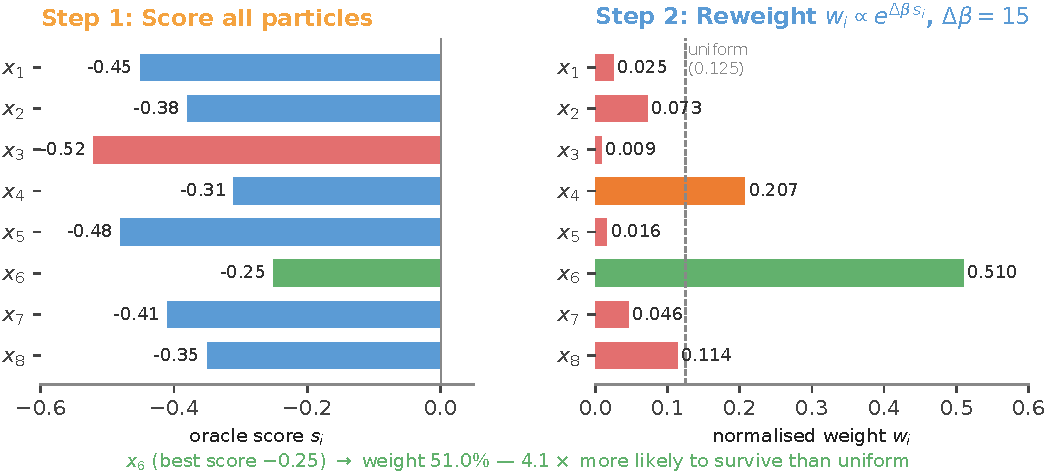
\includegraphics[width=0.95\linewidth]{figures/fig_gpa_walkthrough_score.pdf}
\caption{Score and reweight on the $N\!=\!8$ toy. \textbf{Left:} per-particle oracle scores $s_i$ (best in green: $x_6\!=\!-0.25$; worst in red: $x_3\!=\!-0.52$). \textbf{Right:} normalised weights after the tilt $w_i\!\propto\!\exp(\Delta\beta\,s_i)$ at $\Delta\beta\!=\!15$; uniform $1/N\!=\!0.125$ shown dashed. $x_6$ collects $51.0\%$ of the mass---$4.1\!\times$ the uniform expectation.}
\label{fig:walkthrough-score}
\end{figure}

\subsection{Adapting $\Delta\beta$ via bisection on $\ESS$}

The ESS-adaptive schedule (Lemma~\ref{lem:ess}) chooses $\Delta\beta_t$ so that $\ESS\!\geq\!\alpha N$ \emph{exactly} (not below). With $\alpha\!=\!0.5$, the target is $\ESS_{\rm target}\!=\!4$. Algorithm~\ref{alg:bisect} runs 64 bisection iterations on $[\Delta\beta_{\min}, \Delta\beta_{\max}]\!=\![0,1000]$.

\begin{algorithm}[h]
\caption{Bisection for $\Delta\beta$ given $\ESS$ target}\label{alg:bisect}
\begin{algorithmic}[1]
\State \textbf{Input:} scores $\{r_i\}_{i=1}^N$, target $\tau N$, range $[\Delta\beta_{\min}, \Delta\beta_{\max}]$, max iters $T_{\rm bs}$
\For{$t\!=\!1,\dots,T_{\rm bs}$}
    \State $\Delta\beta_{\rm mid}\!\leftarrow\!(\Delta\beta_{\min}+\Delta\beta_{\max})/2$
    \State $w_i\!\leftarrow\!\exp(\Delta\beta_{\rm mid}\,r_i)/Z$, with $Z\!=\!\sum_j\exp(\Delta\beta_{\rm mid}\,r_j)$
    \State $\ESS\!\leftarrow\!1/\sum_i w_i^2$
    \If{$\ESS > \tau N$} $\Delta\beta_{\min}\!\leftarrow\!\Delta\beta_{\rm mid}$ \Comment{can push harder}
    \Else \;$\Delta\beta_{\max}\!\leftarrow\!\Delta\beta_{\rm mid}$ \Comment{too aggressive}
    \EndIf
\EndFor
\State \textbf{Return:} $\Delta\beta_{\min}$
\end{algorithmic}
\end{algorithm}

For our example, the bisection converges to $\Delta\beta\!\approx\!11.7$, giving $\ESS\!\approx\!4.0\!=\!\alpha N$. The hand-picked $\Delta\beta\!=\!15$ above (which produced $\ESS\!=\!3.08$) was therefore more aggressive than the auto-schedule would choose.

\begin{figure}[h]
\centering
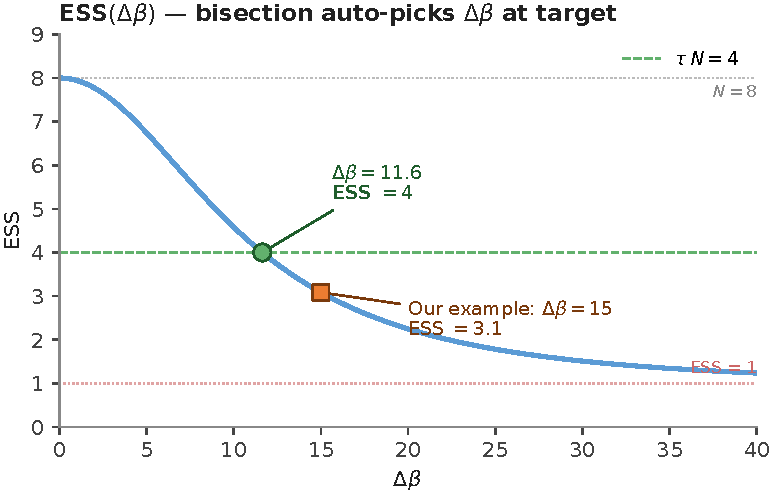
\includegraphics[width=0.78\linewidth]{figures/fig_gpa_walkthrough_ess.pdf}
\caption{$\ESS(\Delta\beta)$ for the $N\!=\!8$ toy oracle scores. The function decreases monotonically from $\ESS\!=\!N$ at $\Delta\beta\!=\!0$ toward $\ESS\!=\!1$ as $\Delta\beta\!\to\!\infty$ (winner-take-all). Bisection finds the unique $\Delta\beta\!=\!11.7$ at which $\ESS$ hits the target $\tau N\!=\!4$ (green dot). The hand-picked $\Delta\beta\!=\!15$ used in the walk-through (orange square) is past the target and so over-collapses the population.}
\label{fig:walkthrough-ess}
\end{figure}

\subsection{Resampling: multinomial vs.\ systematic}

\paragraph{Multinomial.} Draw counts $\!=\!(c_1,\dots,c_N)\!\sim\!\mathrm{Multinomial}(N, w)$. Expected copies per particle are $\E[c_i]\!=\!N\!\cdot\!w_i$, but the realised counts are noisy.

\paragraph{Systematic.} Lay the weights end-to-end as a unit interval $[0,1]$ (segment $i$ has width $w_i$). Drop $N$ pointers at positions $u\!+\!k/N$ for $k\!=\!0,\dots,N\!-\!1$, with $u\!\sim\!\mathrm{Uniform}[0,1/N)$. Particle $i$ receives a number of copies equal to the count of pointers in its segment. This has identical mean to multinomial but lower variance, and is the default in \gpa{}.

For our $N\!=\!8$ example with $u\!=\!0$, the eight pointers at $\{0.000, 0.125, 0.250, 0.375, 0.500, 0.625, 0.750, 0.875\}$ land in segments as follows: $w_2$ (cumulative 0.025--0.098) captures pointer 0.097; $w_4$ (0.107--0.314) captures pointers at 0.125, 0.250; $w_6$ (0.330--0.840) captures pointers at 0.375, 0.500, 0.625, 0.750; $w_8$ (0.886--1.000) captures pointer 0.875. Final copy counts:
\begin{center}
\begin{tabular}{lcccccccc}
\toprule
$i$       & 1 & 2 & 3 & 4 & 5 & 6 & 7 & 8 \\
copies    & 0 & 1 & 0 & 2 & 0 & 4 & 0 & 1 \\
\bottomrule
\end{tabular}
\end{center}
Four particles ($x^1, x^3, x^5, x^7$) are eliminated; $x^6$ is duplicated four times. After resampling, weights reset to $1/N\!=\!0.125$ uniformly.

\begin{figure}[h]
\centering
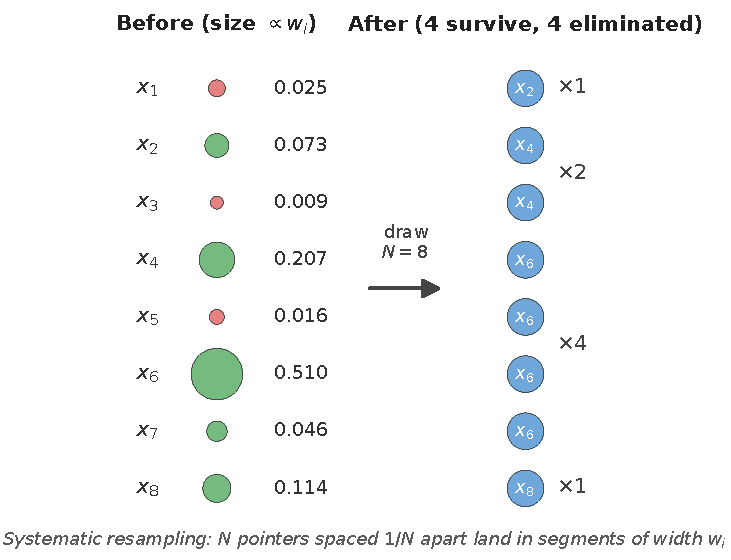
\includegraphics[width=0.85\linewidth]{figures/fig_gpa_walkthrough_resample.pdf}
\caption{Systematic resampling of the $N\!=\!8$ toy. \textbf{Left:} bubble area is proportional to $w_i$; green = retained, red = eliminated by the resampling step. \textbf{Right:} after resampling, all weights reset to $1/N$; $x_6$ now appears four times, $x_4$ twice, $x_2$ and $x_8$ once each. Four particles ($x_1, x_3, x_5, x_7$) are eliminated.}
\label{fig:walkthrough-resample}
\end{figure}

\subsection{Mutation: partial mask + denoise on a length-12 DNA toy}

Each of the eight resampled (now duplicate-rich) particles is independently mutated by $K_\beta$. Concretely, with mask fraction $\mathrm{nf}\!=\!0.25$ ($\!\to\!\lceil 0.25\!\cdot\!12\rceil\!=\!3$ positions on a length-12 sequence):
\begin{center}
\begin{tabular}{ll}
\toprule
\textbf{Step}        & \textbf{Sequence} \\
\midrule
Before (a duplicate of $x^6$)   & \texttt{ACGTATGCACGT} \\
Random mask 3 positions          & \texttt{AC?TA?GC?CGT} \\
Denoise via $p_\theta$           & \texttt{AC\textbf{T}TA\textbf{A}GC\textbf{A}CGT} \\
\midrule
Net edits                         & pos 3: G$\to$T; \, pos 6: T$\to$A; \, pos 9: C$\to$A \\
\bottomrule
\end{tabular}
\end{center}
Two properties this kernel inherits from the pretrained $p_\theta$:
\begin{itemize}
\item \emph{Grammar preservation.} The denoiser sees the unmasked context and proposes tokens consistent with whatever motif/composition rules $p_\theta$ has learned. Random per-position resampling would not.
\item \emph{Diversity restoration.} The four duplicates of $x^6$ each get an \emph{independent} random mask + denoising pass, so they diverge into four distinct child sequences. Without mutation the population would collapse to four identical copies.
\end{itemize}
The mask fraction $\mathrm{nf}$ controls exploration: $\mathrm{nf}\!=\!0.05$ is local search ($\sim\!10$ positions per step on a 200-bp DNA enhancer), $\mathrm{nf}\!=\!0.20$ is large jumps. Section~\ref{sec:results:ablation} reports sensitivity in the practical range.

%-----------------------------------------------------------------------
\section{Hyperparameters}\label{app:hyper}

Table~\ref{tab:hyper-rerd} lists hyperparameters for the SMC-protocol comparison (\drakes{} eval pair); Table~\ref{tab:hyper-ctrldna} lists those for \ctrldna{} comparison (HyenaDNA + gReLU MSE oracles); Table~\ref{tab:hyper-dnacraft} for \dnacraft{} comparison (HyenaDNA/DiMamba + Enformer 50/50). Default values are bolded.

\begin{table}[h]
\caption{Hyperparameters for the SMC-protocol comparison (HepG2 enhancer, MDLM backbone, \drakes{} split-oracle).}
\label{tab:hyper-rerd}
\centering
\small
\begin{tabular}{lll}
\toprule
Parameter & Mean recipe & Spec recipe \\
\midrule
$N$ (population) & 5000 & 5000 \\
$\alpha$ (ESS threshold) & 0.5 & 0.5 \\
$\beta_*$ (target inverse temp) & 200 & 100 \\
$T_{\max}$ (max steps) & 30, hard cap 200 & 30, hard cap 200 \\
nf (mask fraction) & 0.05 & 0.05 \\
DPS gradient strength $\eta$ & 3000 & 3000 \\
$\mathrm{pw}$ (off-target penalty) & 0 & 0.35 \\
GC bio-filter & [0.45, 0.55] & [0.45, 0.55] \\
\bottomrule
\end{tabular}
\end{table}

\begin{table}[h]
\caption{Hyperparameters for \ctrldna{} comparison (Reddy promoters, HyenaDNA backbone, gReLU MSE oracles, universal recipe).}
\label{tab:hyper-ctrldna}
\centering
\small
\begin{tabular}{ll}
\toprule
Parameter & Universal recipe \\
\midrule
$N$ (population) & 10000 \\
$\alpha$ (ESS threshold) & 0.5 \\
$\beta_*$ & 100 \\
$T_{\max}$ (steps) & 60 \\
nf (mask fraction) & 0.05 \\
$K$ (branch factor) & 8 \\
$\mathrm{pw}$ & 0.35 \\
diversity $\lambda$ (conformity) & \textbf{1.0} \\
DPS & off \\
GC bio-filter & off \\
\bottomrule
\end{tabular}
\end{table}

\begin{table}[h]
\caption{Hyperparameters for \dnacraft{} comparison (Gosai 50/50 split, top-128 by MinGap-Eval). C1 = no GC penalty; C3 = soft GC penalty (gct=0.60), no hard bio-filter.}
\label{tab:hyper-dnacraft}
\centering
\small
\begin{tabular}{lll}
\toprule
Parameter & C1 & C3 \\
\midrule
$N$ (population) & 5000 & 5000 \\
$\beta_*$ & 25 & 25 \\
$\mathrm{pw}$ & 0.30 & 0.30 \\
DPS & on & on \\
GC penalty (gct) & --- & 0.60 \\
GC bio-filter & off & off \\
$K$ & 8 & 8 \\
\bottomrule
\end{tabular}
\end{table}

%-----------------------------------------------------------------------
\section{Full GPA-vs-ISM/LEDIDI tables}\label{app:ism_full}

Single-sequence comparison: GPA row = the one sequence in each pool that maximises $\mathrm{AG}-\mathrm{LN}$ (sweet spot: low LN, high held-out AG). Directly comparable to \ism{}/\ledidi{} which are inherently single-sequence.

\begin{table}[h]
\caption{Single-sequence comparison, K562 enhancer, two seeds (uid=181692 natural, uid=50178 random). \gpa{} row = argmax of $\mathrm{AG}-\mathrm{LN}$ within the 5{,}000-seq pool.}
\label{tab:ism_singleseq}
\centering
\small
\begin{tabular}{llrrr}
\toprule
Seed & Method & Edits & LN & AG \\
\midrule
\multirow{4}{*}{uid=181692}
 & \gpa{} (no DPS) uncap   &  96 & 4.97 & \textbf{3.33} \\
 & \gpa{} (+DPS) cap30     &  60 & 6.21 & \textbf{3.47} \\
 & \ism{} gen 115          & 115 & 8.74 & 2.83 \\
 & \ledidi{} t15 $\lambda$=0.05 & 125 & 9.81 & $-$0.22 \\
\midrule
\multirow{4}{*}{uid=50178}
 & \gpa{} (no DPS) cap30   &  60 & 4.71 & 2.75 \\
 & \gpa{} (+DPS) cap30     &  59 & 6.58 & \textbf{3.61} \\
 & \ism{} gen 115          & 115 & 9.58 & 2.92 \\
 & \ledidi{} t15 $\lambda$=0.05 & 105 &11.66 & $-$0.62 \\
\bottomrule
\end{tabular}
\end{table}

\paragraph{Reading the table.}
A single \gpa{} sequence (e.g.\ +DPS cap30 on uid=50178: LN $6.58$, AG $3.61$) beats \ism{} gen 115 on the held-out AG by $+0.69$ at LN $\sim\!3.0$ lower—better held-out activity \emph{and} less reward-hacking. Under any selection rule, \ledidi{} stays AG-negative; not one of its 50 reruns produces an AG-positive sequence.

\paragraph{Apples-to-apples runtime (single H100, K562 enhancer, 5{,}000-sequence pool).}
Table~\ref{tab:ism_runtime} reports wall-time at matched output volume, averaged across the random and natural pools. \gpa{} is fully population-parallel: a single SMC step propagates all 5{,}000 particles together through the diffusion proposal, so the per-particle cost is the GPU-memory chunk \texttt{mutation\_batch\_size=128} amortised over the population. \ism{} is also nominally population-parallel (5{,}000 independent greedy trajectories), but its sequential cost is fixed at 115 generations per seed, and that dominates wall regardless of how memory chunks are batched. \ledidi{} is chunked-sequential by design: 5{,}000 seeds processed in 39 chunks of 128 along the Gumbel-softmax optimisation. The result is $\sim\!9.3\times$ speedup over \ism{} and $\sim\!3.4\times$ speedup over \ledidi{} at identical pool size and identical hardware.

\begin{table}[h]
\caption{Apples-to-apples runtime: single H100, 5{,}000-sequence K562-enhancer pool, averaged across random and natural seed pools. \gpa{} = v3 noDPS recipe (matches Sec.~\ref{sec:results:ism}). Speedup column is $\mathrm{wall}_{\text{baseline}}/\mathrm{wall}_{\gpa{}}$.}
\label{tab:ism_runtime}
\centering
\small
\begin{tabular}{lllr}
\toprule
Method & Wall (5K pool) & Parallelism & Speedup vs.\ \gpa{} \\
\midrule
\textbf{\gpa{}} & \textbf{$\sim\!11.6$ min} & population-parallel (5{,}000 SMC particles) & --- \\
\ledidi{}       & $\sim\!40$ min     & chunked-sequential (39 chunks $\times$ 128 seeds) & $\sim\!3.4\times$ slower \\
\ism{}          & $\sim\!107.5$ min  & population-parallel, but 115 sequential greedy gens & $\sim\!9.3\times$ slower \\
\bottomrule
\end{tabular}
\end{table}

%-----------------------------------------------------------------------
\section{Full DNA-CRAFT tables (GPA-C1 vs GPA-C3)}\label{app:dnacraft_full}

The headline column in Table~\ref{tab:dnacraft} uses GPA-C3 (\texttt{dps\_pw030\_b25\_gct060\_nobio}). This appendix shows the same benchmark with the alternate recipe variant GPA-C1 (\texttt{dps\_pw030\_b25}, no GC penalty), under the matched-output-budget protocol of Table~\ref{tab:dnacraft} (\texttt{by\_pool\_composite} top-64 from \texttt{gpa\_output\_best\_eval.h5}, 3 reps for both variants). Both variants run at $\sim\!3.6$ min/seed (no MCTS) on the MDLM backbone; the only difference is the soft GC-centering term added to C3's DPS gradient.

\paragraph{Recipe decomposition.}
Each token in the recipe name maps to a specific knob in the GPA algorithm of \S\ref{sec:method}, with no other differences between the two variants:
\begin{itemize}
\item \texttt{dps} -- enables the Gumbel-softmax oracle gradient with strength $\eta\!=\!3000$ (\S\ref{sec:method:ext}, ``Gumbel-softmax oracle gradient (DPS)''). This is a biased proposal in the sense of \S\ref{sec:method:ext} and is shared by both C1 and C3, so the C1$\leftrightarrow$C3 contrast does not move along the DPS-bias axis.
\item \texttt{pw030} -- sets the off-target weight $\mathrm{pw}\!=\!0.30$ in the linear fitness of Eq.~\ref{eq:fitness} (\S\ref{sec:method:pw}); the same $0.30$ weights the off-target term inside the DPS gradient as well.
\item \texttt{b25} -- sets the SMC tilt ceiling $\beta_*\!=\!25$. This is below the default range $\beta_*\!\in\!\{100,200\}$ in \S\ref{sec:exp} and is a deliberately gentler tilt that preserves population diversity at some cost in MinGap; both variants share it.
\item \texttt{gct060} \emph{(C3 only)} -- adds a quadratic centering term $-w\,(g(x)-0.60)^2$ to the DPS objective before backpropagation, where $g(x)\!=\!\overline{P(C)+P(G)}$ is the per-position soft-onehot GC fraction and $w\!=\!10$. The penalty rides inside the same Gumbel-softmax gradient that DPS already computes; it is \emph{not} a hard accept/reject filter.
\item \texttt{nobio} -- disables the hard bio-filter (no \texttt{gc\_low}/\texttt{gc\_high} interval gating). All GC discipline in C3 therefore comes from the soft \texttt{gct060} term in the DPS gradient.
\end{itemize}
Both variants additionally use the default branch factor $K\!=\!8$ (\S\ref{sec:method:ext}, Prop.~\ref{prop:K}) and population $N\!=\!5{,}000$ (Table~\ref{tab:dnacraft} caption), so both target $\pi_{\beta_*}^{(K=8)}\!\neq\!\pi_{\beta_*}$ in the sense of Prop.~\ref{prop:K}; the C1$\leftrightarrow$C3 contrast isolates the GC-centering term with $K$, $\beta_*$, $\mathrm{pw}$, $N$, and the DPS bias all held constant.

\begin{table}[h]
\caption{\dnacraft{} benchmark with the GPA-C1 alternate recipe (\texttt{dps\_pw030\_b25}; no GC penalty), reported alongside the headline GPA-C3 (Table~\ref{tab:dnacraft}). Both columns: \texttt{by\_pool\_composite} top-64 from \texttt{gpa\_output\_best\_eval.h5}, mean (std) over 3 reps. Baselines verbatim from \citet{dnacraft2026}.}
\label{tab:dnacraft_full_eval}
\centering
\scriptsize
\begin{tabular}{llcccccccccc}
\toprule
Cell & Metric & SMC & CG & TDS & DRAKES & D3 & Ledidi & Ctrl-DNA & DNA-CRAFT & \gpa{}-C1 & \gpa{}-C3 \\
\midrule
\multirow{4}{*}{HepG2}
 & MinGap   & 1.61 & $-$0.23 & 0.40 & $-$1.40 & 0.05 & 5.77 & \textbf{7.79} & 4.35 & 6.87 & 6.91 \\
 & Motif    & 0.55 & 0.86 & 0.40 & 0.06 & 0.87 & 0.58 & 0.63 & \textbf{0.92} & 0.90 & \textbf{0.92} \\
 & 3-mer    & 0.81 & 0.97 & 0.74 & $-$0.36 & \textbf{0.98} & 0.76 & 0.49 & \textbf{0.98} & 0.95 & 0.95 \\
 & Diversity& 0.83 & \textbf{1.98} & 0.96 & 1.86 & \textbf{1.98} & \textbf{1.98} & 1.90 & \textbf{1.98} & 1.81 & 1.86 \\
\midrule
\multirow{4}{*}{K562}
 & MinGap   & 4.12 & 0.00 & 1.62 & $-$0.20 & 0.18 & 7.66 & \textbf{9.07} & 5.69 & 8.18 & 8.13 \\
 & Motif    & 0.45 & 0.85 & 0.51 & 0.14 & 0.86 & 0.65 & 0.63 & 0.93 & 0.93 & \textbf{0.94} \\
 & 3-mer    & 0.66 & 0.94 & 0.65 & $-$0.35 & 0.96 & 0.69 & 0.41 & \textbf{0.98} & 0.92 & 0.95 \\
 & Diversity& 0.31 & \textbf{1.98} & 0.64 & 1.96 & \textbf{1.98} & \textbf{1.98} & 1.90 & \textbf{1.98} & 1.56 & 1.83 \\
\midrule
\multirow{4}{*}{SK-N-SH}
 & MinGap   & 0.56 & $-$0.28 & 0.19 & 0.09 & $-$0.01 & 3.03 & 3.72 & 3.23 & \textbf{5.07} & 4.98 \\
 & Motif    & 0.52 & 0.86 & 0.48 & 0.23 & 0.84 & 0.38 & 0.48 & 0.88 & 0.89 & \textbf{0.92} \\
 & 3-mer    & 0.78 & 0.95 & 0.72 & $-$0.38 & 0.93 & 0.37 & 0.20 & \textbf{0.97} & 0.87 & 0.94 \\
 & Diversity& 1.27 & \textbf{1.98} & 0.92 & 1.83 & 1.97 & \textbf{1.98} & 1.86 & \textbf{1.98} & 1.59 & 1.86 \\
\bottomrule
\end{tabular}
\end{table}

\paragraph{Reading.}
GPA-C1 and GPA-C3 give nearly tied MinGap and Motif Spearman on every cell (within seed std on most rows). C3 wins Motif on HepG2 / K562 / SK-N-SH ($+0.02$/$+0.01$/$+0.03$) and 3-mer on K562 / SK-N-SH ($+0.03$/$+0.07$). The biggest practical difference is Diversity: the soft GC-centering term in C3's DPS gradient recovers $+0.05$ to $+0.27$ Shannon bits over C1 on every cell, lifting C3 above the Ctrl-DNA Diversity floor on all three cells. The mechanism is indirect: by penalising drift away from $g(x)\!=\!0.60$ at every Gumbel-softmax step, the term blunts the oracle's tendency to push particles toward narrow high-GC modes, which in turn keeps the population spread out in sequence space. C1 wins MinGap on K562 / SK-N-SH ($+0.05$/$+0.09$) but loses across the rest. C3 is the headline because the +Diversity / +Motif / +3-mer trade dominates the small MinGap give-back; C1 is reported as an ablation that isolates the GC-penalty's contribution.

\paragraph{Backbone caveat.}
\dnacraft{}'s reported numbers in Table~\ref{tab:dnacraft} are obtained on a Mamba-style discrete-diffusion (DiMamba) backbone whose code and pretrained checkpoints are not publicly available; the same paper also reports DiMamba-vs-MDLM ablations that show DiMamba contributes additional biological-faithfulness gains. Our \gpa{}-C1 / \gpa{}-C3 numbers are obtained on the publicly available MDLM backbone of \citet{sahoo2024mdlm} and should be read as a lower bound on what \gpa{} would achieve at backbone parity, by Remark~\ref{rem:agnostic}.

%-----------------------------------------------------------------------
\section{Wall-time table}\label{app:wall}

\begin{table}[h]
\caption{Wall time per seed and 5-seed totals (HepG2, identical H100 hardware, identical HyenaDNA backbone). Wall time excludes downstream motif scoring.}
\label{tab:wall}
\centering
\small
\begin{tabular}{lrr}
\toprule
Method & Wall/seed (h) & 5-seed total (GPU-h) \\
\midrule
\ctrldna{} R200 (RL fine-tune) & $43.5\pm 0.8$ & $\sim\!218$ \\
\gpa{} v3 (K=8, no diversity)  & $3.97\pm 0.59$ & 19.8 \\
\gpa{} v4 (K=8 + rejuvenation) & $2.17\pm 0.22$ & 10.8 \\
\gpa{} v5 (K=8 + diversity)    & $\mathbf{2.22\pm 0.52}$ & $\mathbf{11.1}$ \\
\bottomrule
\end{tabular}
\end{table}

%-----------------------------------------------------------------------
\section{DPS gradient ablation}\label{app:dps_ablation}

Population annealing alone (no DPS) already beats single-chain refinement baselines; DPS gradient is a multiplicative enhancement.

\begin{table}[h]
\caption{DPS gradient ablation on Gosai HepG2.}
\label{tab:dps_ablation}
\centering
\small
\begin{tabular}{llrrr}
\toprule
Track & Metric & \gpa{}-only & \gpa{}+DPS & $\Delta$(DPS) \\
\midrule
Mean & $H_{\mathrm{eval}}$ & $8.73\pm 0.50$ & $\mathbf{10.06\pm 0.19}$ & $+1.33$ \\
Mean & Spec & 1.58 & 3.06 & $+1.48$ \\
Spec & $H_{\mathrm{eval}}$ & $8.28\pm 0.12$ & $9.35\pm 0.20$ & $+1.07$ \\
Spec & Spec & $6.11\pm 1.45$ & $\mathbf{7.61\pm 0.25}$ & $+1.50$ \\
\bottomrule
\end{tabular}
\end{table}

%-----------------------------------------------------------------------
\section{Naturalness audit}\label{app:naturalness}

\begin{table}[h]
\caption{Naturalness audit (HepG2 top-128). \gpa{} produces bio-plausible sequences by construction; \ctrldna{} reward-hacks to non-biological space.}
\label{tab:nat}
\centering
\small
\begin{tabular}{lrrr}
\toprule
Metric & Real (Gosai) & \gpa{} & \ctrldna{} \\
\midrule
GC mean & 0.44 & 0.41 & 0.45 \\
\textbf{bio\_pass\_rate} & 0.51 & $\mathbf{1.00}$ & $\mathbf{0.05}$ \\
max homopolymer & 5.4 & 5.1 & $\mathbf{20.9}$ \\
$k$=3 Pearson & 1.0 & 0.61 & 0.39 \\
HNF1A enrichment & $0\times$ & $10\,040\times$ & $7\,812\times$ \\
\bottomrule
\end{tabular}
\end{table}

\begin{figure}[h]
\centering
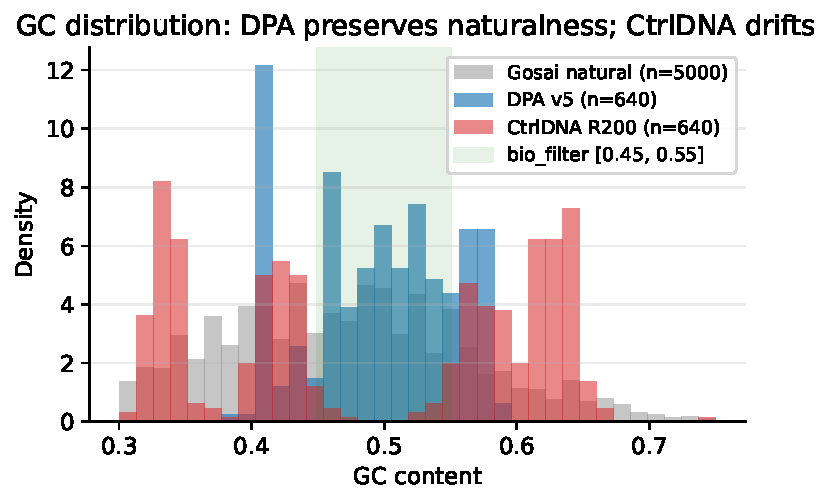
\includegraphics[width=0.6\linewidth]{figures/fig2_gc.pdf}
\caption{GC distribution comparison on HepG2 top-128 sequences. \gpa{} (blue) clusters near the lower edge of the bio-filter (45\%) but stays within the natural Gosai range (gray); \ctrldna{} (red) drifts widely, with a heavy tail of low- and high-GC sequences and a substantial fraction outside the natural distribution.}
\label{fig:gc}
\end{figure}

%-----------------------------------------------------------------------
\section{Extreme specificity}\label{app:extreme}

Pushing $\mathrm{pw}$ beyond the canonical $0.35$ trades $H_{\mathrm{eval}}$ for higher specificity until both off-targets fall below baseline (Table~\ref{tab:extreme}).

\begin{table}[h]
\caption{Extreme-specificity extension on Gosai HepG2 (single run each, $N\!=\!5000$).}
\label{tab:extreme}
\centering
\small
\begin{tabular}{rrrrr}
\toprule
$\mathrm{pw}$ & $H_{\mathrm{eval}}$ & $K_{\mathrm{eval}}$ & $S_{\mathrm{eval}}$ & $H{>}8 \wedge K{<}0 \wedge S{<}0$ \\
\midrule
0.35 & 9.65 & 2.15 &  1.10 & 0 \\
0.50 & 9.54 & 1.96 &  0.63 & 0 \\
0.70 & 8.73 & 1.52 &  0.35 & 0 \\
1.00 & 8.57 & 0.69 & $-$0.48 & 26 \\
1.50 & $\mathbf{8.44}$ & 0.55 & $\mathbf{-0.66}$ & $\mathbf{54}$ \\
\bottomrule
\end{tabular}
\end{table}

\paragraph{Beta trajectory.}
Figure~\ref{fig:beta} shows a representative ESS-adaptive $\beta$ trajectory and the population-mean reward over SMC steps for a HepG2 run.

\begin{figure}[h]
\centering
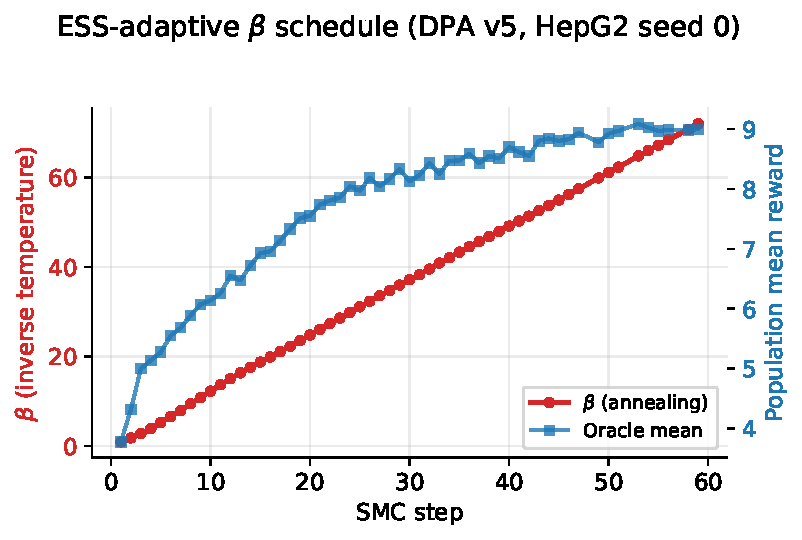
\includegraphics[width=0.6\linewidth]{figures/fig4_beta_traj.pdf}
\caption{Representative \gpa{} run trajectory (HepG2, seed 0). Red trace: ESS-adaptive $\beta$ schedule rises through the annealing path. Blue trace: population mean reward grows monotonically toward saturation as $\beta$ increases.}
\label{fig:beta}
\end{figure}

%-----------------------------------------------------------------------
\section{Negative result: APF correction for $\epsilon$-greedy $K$-branching}\label{app:apf}

A natural attempt to recover Shannon under $K$-branching is to soften the argmax with $\epsilon$-greedy ($\tau\!>\!0$ softmax over the $K$ siblings) and apply the auxiliary-particle-filter weight correction \citep{pittshephard1999}:
\[
w_{\mathrm{new}} = w_{\mathrm{old}}\big/p_\tau(\mathrm{winner}),\qquad p_\tau(j)=\exp(r_j/\tau)\big/\sum_m\exp(r_m/\tau).
\]
Compute the expectation:
\[
\E[w_{\mathrm{new}}\,\varphi(x_{\mathrm{winner}})] = \E_{x_{1:K}\sim q}\!\!\left[\sum_{j=1}^K \frac{\exp(r_j/\tau)}{\sum_m\exp(r_m/\tau)}\cdot\frac{\sum_m\exp(r_m/\tau)}{K\exp(r_j/\tau)}\,\varphi(x_j)\right]=\frac{1}{K}\sum_j \E_q[\varphi(x_j)],
\]
i.e.\ the corrected estimator is equivalent to a single-child sample. The $K$ siblings collapse and the effective-$\beta$ boost vanishes. Empirically, on a synthetic linear reward $r(x)\!=\!3x$ with $q$ uniform on $[0,1]$ (200K Monte-Carlo trials):
\begin{center}
\small
\begin{tabular}{lrrr}
\toprule
Variant & $\E[x]$ & $\mathrm{Var}[x]$ & ESS \\
\midrule
$K=1$ no selection                & 0.5000 & 0.0833 & 100.0\% \\
$K=8$ argmax (no correction)      & 0.8887 & 0.0099 & 100.0\% \\
$K=8$ softmax $\tau\!=\!0.3$ (no corr.) & 0.8445 & 0.0180 & 100.0\% \\
\textbf{$K=8$ softmax $\tau\!=\!0.3$ + APF} & 0.4880 & 0.0874 & 0.4\% \\
$K=8$ softmax $\tau\!=\!1.0$ + APF & 0.5009 & 0.0829 & 53.1\% \\
\bottomrule
\end{tabular}
\end{center}
ESS collapses at low $\tau$ and the corrected mean/variance reproduces $K=1$. We therefore do \emph{not} use APF correction for production runs and report only argmax $K$-branching. K-annealing schedules and waste-free SMC \citep{dau2022wastefree} remain valid theoretical alternatives, deferred to future work.

%-----------------------------------------------------------------------
\section{Negative result: post-hoc Metropolis tempering}\label{app:posthoc}

Another natural Shannon-rescue move is to load the concentrated argmax-$K$ pool and run Metropolis–Hastings at lower $\beta'$ to spread the population. We tested this on the K562 promoter pool (50 MH steps, nf=0.05, HyenaDNA proposal):

\begin{center}
\small
\begin{tabular}{rrrrr}
\toprule
$\beta'$ & accept rate & $\Delta$comp & $\Delta$tgt & $\Delta H$ \\
\midrule
25 &  3.4\% & $+0.02$ & $-0.06$ & $+0.05$ \\
12 &  6.5\% & $-0.15$ & $-0.27$ & $+0.10$ \\
 6 & 13.1\% & $-0.68$ & $-0.77$ & $+0.21$ \\
 3 & 29.1\% & $-2.12$ & $-2.22$ & $+0.39$ \\
 1 & 73.7\% & $-4.71$ & $-5.35$ & $+0.61$ \\
\bottomrule
\end{tabular}
\end{center}
The Pareto slope is $\sim\!3\!-\!5$ target units per $0.1$ nat of Shannon, far too steep for the diversity gap to \dnacraft{}/\ctrldna{} K562 ($\sim\!0.5$ nat) to be closed without erasing the target advantage. Increasing chain length or shrinking nf does not change the local-neighborhood geometry. The honest reading: under sharply peaked oracles, the activity–diversity tension is in the reward landscape, not the sampler.

%-----------------------------------------------------------------------
\section{GC distribution and floor-hugging}\label{app:gc}

Even with the bio-filter $\mathrm{GC}\!\in\![0.45,0.55]$, $60\!-\!75\%$ of \gpa{} top-128 sequences cluster at the lower bound. Two facts:
\begin{enumerate}
\item This is a property of the \emph{masked-diffusion proposal} at low noise fraction. At $\mathrm{nf}\!=\!0.20$ the bias inverts toward the upper bound (GC $\approx\!0.54$); the crossover occurs near $\mathrm{nf}\!\approx\!0.16\!-\!0.17$.
\item The eval oracle is GC-agnostic: at both $\mathrm{nf}$ extremes, top-128 oracle scores are comparable. The GC bias arises from $p_\theta$, not from the reward signal.
\end{enumerate}
Three mitigations were tested with mixed success: (i) GC-aware DPS gradient (\verb|gc_dps_weight|) reduces floor-hugging from $61.5\%$ to $55.0\%$ at $-0.09$ $H_{\mathrm{eval}}$ cost; (ii) narrow $1\%$ GC bands achieve uniform GC by construction at $-0.25$ $H_{\mathrm{eval}}$; (iii) stratified resampling within $2\%$ GC bins \citep{verge2015island} achieves balanced coverage at $-0.50$ to $-1.0$ $H_{\mathrm{eval}}$. We report all three options in the codebase but use the unmitigated baseline in the headline tables for fair comparison with peer methods.

%-----------------------------------------------------------------------
\section{Ctrl-DNA enhancer comparison (V7 main + V5/V8 ablations)}\label{app:ctrldna_enhancer}

This appendix gives the dedicated \ctrldna{}-vs-\gpa{} enhancer comparison referenced in \S\ref{sec:results:promoter}. Same Gosai 50/50 split as the \dnacraft{} benchmark, top-128 selection per cell, 5 \gpa{} seeds. The headline GPA recipe is V7 (universal: $K\!=\!8$, diversity $\lambda\!=\!1.0$); V8a, V8b (alternative pairwise-suppression formulations) and V5 (the previous default with $\lambda\!=\!0.2$) are ablations.

\begin{table}[h]
\caption{Ctrl-DNA vs.\ \gpa{} on Gosai HepG2/K562/SKNSH enhancers (5 seeds; mean (std)). Headline = V7 universal recipe; V8a (log\_ratio + pw=1.0), V8b (linear + pw=1.0) and V5 ($\lambda\!=\!0.2$) are ablations of the diversity / pairwise-suppression knob. \texttt{target\_raw} = mean target oracle score; \texttt{ΔR} = normalised target minus mean off-target; \texttt{shannon} = per-position entropy; \texttt{motif\_corr} = FIMO Pearson against per-cell real reference.}
\label{tab:ctrldna_enhancer}
\centering
\footnotesize
\setlength{\tabcolsep}{4pt}
\begin{tabular}{llrrrr}
\toprule
Cell & Method & target\_raw $\uparrow$ & ΔR $\uparrow$ & shannon $\uparrow$ & motif\_corr $\uparrow$ \\
\midrule
\multirow{5}{*}{HepG2}
 & \ctrldna{} R200             & 5.32 (0.65) & 0.48 (0.10) & 1.65 (0.14) & \textbf{0.29} (0.16) \\
 & \gpa{} V5 ($K\!=\!8, \lambda\!=\!0.2$) & 9.86 (0.10) & 0.85 (0.01) & 1.49 (0.03) & 0.19 (0.03) \\
 & \gpa{} V7 ($K\!=\!8, \lambda\!=\!1.0$) & \textbf{9.90} (0.12) & 0.84 (0.02) & 1.59 (0.11) & 0.20 (0.02) \\
 & \gpa{} V8a (log\_ratio, pw=1.0) & 6.61 (0.04) & 0.68 (0.01) & \textbf{1.93} (0.00) & 0.15 (0.02) \\
 & \gpa{} V8b (linear, pw=1.0) & 9.51 (0.10) & \textbf{0.93} (0.02) & 1.70 (0.11) & 0.10 (0.04) \\
\midrule
\multirow{5}{*}{K562}
 & \ctrldna{} R200             & \textbf{9.99} (1.52) & \textbf{0.77} (0.14) & 1.60 (0.15) & 0.24 (0.07) \\
 & \gpa{} V5 ($K\!=\!8, \lambda\!=\!0.2$) & 8.82 (0.13) & 0.34 (0.00) & 1.43 (0.09) & \textbf{0.26} (0.02) \\
 & \gpa{} V7 ($K\!=\!8, \lambda\!=\!1.0$) & 8.83 (0.12) & 0.32 (0.01) & 1.65 (0.02) & 0.24 (0.02) \\
 & \gpa{} V8a (log\_ratio, pw=1.0) & 6.48 (0.03) & 0.39 (0.01) & \textbf{1.94} (0.01) & 0.24 (0.01) \\
 & \gpa{} V8b (linear, pw=1.0) & 8.15 (0.04) & 0.41 (0.01) & 1.68 (0.02) & 0.25 (0.02) \\
\midrule
\multirow{5}{*}{SK-N-SH}
 & \ctrldna{} R200             & 9.93 (1.13) & \textbf{0.71} (0.10) & 1.63 (0.17) & \textbf{0.23} (0.10) \\
 & \gpa{} V5 ($K\!=\!8, \lambda\!=\!0.2$) & \textbf{14.33} (0.20) & 0.10 (0.01) & 1.49 (0.04) & \textbf{0.23} (0.01) \\
 & \gpa{} V7 ($K\!=\!8, \lambda\!=\!1.0$) & 14.17 (0.18) & 0.10 (0.00) & 1.63 (0.04) & 0.20 (0.01) \\
 & \gpa{} V8a (log\_ratio, pw=1.0) & 6.29 (0.08) & 0.22 (0.01) & \textbf{1.91} (0.01) & 0.15 (0.01) \\
 & \gpa{} V8b (linear, pw=1.0) & 8.26 (0.15) & 0.29 (0.03) & 1.74 (0.05) & 0.10 (0.01) \\
\bottomrule
\end{tabular}
\end{table}

\paragraph{Headlines.}
\gpa{} V7 (the universal recipe) wins target\_raw on HepG2 and SK-N-SH ($+4.58$ and $+4.24$ over \ctrldna{}), and is competitive on K562 within $\sim$1 std. \ctrldna{} retains a ΔR (specificity) edge on K562 and SK-N-SH at the cost of $\sim$50\% lower target activity on HepG2/SK-N-SH and high seed-to-seed variance ($\pm 1.13$--$1.52$). The V7 vs.\ V5 comparison shows the diversity-$\lambda$ bump (from $0.2$ to $1.0$) buys $+0.10$--$0.22$ shannon on every cell at zero target cost, isolating the population-conformity penalty as a strict Pareto improvement. V8a/V8b are alternative pairwise-suppression formulations: V8a (log-ratio reward, pw=1.0) achieves the tightest shannon ($1.91$--$1.94$, near uniform) but at substantial target cost; V8b (linear, pw=1.0) recovers HepG2/K562 target while maximising HepG2 ΔR. The four GPA variants together trace a Pareto front in (target, shannon, motif) space at fixed inference cost---one knob per recipe, no retraining.

%-----------------------------------------------------------------------
\section{DNA-CRAFT $K$ and $i$ scaling sweeps (UCB-MCTS variant)}\label{app:ucb_scaling}

\paragraph{Why MCTS at all.}
DNA-CRAFT replaces the SMC population with a single depth-bounded Monte Carlo Tree Search loop on a DiMamba diffusion backbone, and shows that this delivers state-of-the-art motif and 3-mer grammar fidelity on the Gosai enhancer benchmark (Table~\ref{tab:dnacraft}). The mechanism that delivers their grammar bar is plausible on its face: tree search amortises the cost of choosing the right next mutation by replaying the same scoring oracle across multiple competing children before committing—a strictly more informed proposal than picking the first child that scores well. \gpa{}'s standard $K$-branch is a depth-1 special case of this idea: try $K$ candidates from the proposal and keep the best (Sec.~\ref{sec:method:ext}). It is natural to ask whether the same \emph{deeper} planning that powers \dnacraft{}'s grammar—expanding the best leaves over multiple iterations rather than just one---closes \gpa{}'s residual gap to \dnacraft{} on motif/3-mer correlation. The \texttt{ucb\_stacked} variant exists to test exactly that question.

\paragraph{What \texttt{ucb\_stacked} does, step by step.}
At every SMC mutation step, each particle $x_t^{(j)}$ becomes the root of an independent Monte Carlo tree. We then run $i$ iterations on that tree, where each iteration follows the standard four-phase MCTS-with-UCB1 loop \citep[``UCT'';][]{kocsis2006uct}:
\begin{enumerate}
\item \emph{Selection.} Traverse from the root to a leaf by greedily picking, at each internal node $v$ with already-expanded children $\{a\}$, the child that maximises the UCB1 score \citep{auer2002ucb,kocsis2006uct}
\begin{equation}\label{eq:ucb1}
    \mathrm{UCB1}(a) \;=\; \bar{Q}(a) \;+\; c\sqrt{\frac{\ln n(v)}{n(a)}},
\end{equation}
where $\bar{Q}(a)\!\in\![0,1]$ is the mean (range-normalised) reward backed up through child $a$, $n(a)$ is the visit count of $a$, $n(v)\!=\!\sum_a n(a)$ is the parent visit count, and $c\!=\!\sqrt{2}$ is the standard exploration constant. The first term exploits children with high empirical value; the second term explores low-visit children with a $\sqrt{\log n / n(a)}$ confidence radius. Together this is the canonical bandit rule of \citet{auer2002ucb} for stochastic multi-armed bandits, and \citet{kocsis2006uct} show that applying it node-wise inside a tree (UCT) inherits the same $\mathcal{O}(\log n)$ regret bound at each node. Children with $n(a)\!=\!0$ are tried first by convention so the second term remains well-defined.
\item \emph{Expansion.} Apply \gpa{}'s standard $K$-branch operator at the selected leaf: draw $K\!=\!8$ children using partial-mask$\circ$denoise + DPS (the same operator the no-MCTS \gpa{} would use as its mutation kernel).
\item \emph{Evaluation.} Score each new child under the eval-side reward.
\item \emph{Backpropagation.} Update visit counts $n(\cdot)$ and value estimates $\bar{Q}(\cdot)$ along the path from each new child up to the root, so the next iteration's UCB1 selection (Eq.~\ref{eq:ucb1}) uses fresh statistics.
\end{enumerate}
We bound the tree depth at $d\!=\!2$, so the planner looks at most two mutation steps ahead. After $i$ iterations the tree has at most $1\!+\!i\!\cdot\!K$ nodes; the mutated state for $x_t^{(j)}$ is the highest-reward leaf in that tree. The SMC step then proceeds as usual: the new particle states are importance-weighted at the next $\beta$, resampled if $\ESS$ degenerates, and the loop continues.

\paragraph{Connection to \dnacraft{}.}
The four-step loop (UCB selection $\to$ $K$-fold expansion $\to$ scoring $\to$ reward backprop) is identical in shape to \dnacraft{}'s tree search. What differs is the \emph{scope} of where the tree sits and how it is consumed:
\begin{itemize}
\item \dnacraft{} runs \emph{one} MCTS for the whole design problem: $N_{\mathrm{iter}}\!=\!64$ iterations, $M\!=\!128$ children per expansion, full leaf-to-clean rollouts. Their MinGap-Set archive accumulates the best $N_{\max}\!=\!64$ leaves seen during the run, and that archive is the output (no SMC, no population).
\item \texttt{ucb\_stacked} runs \emph{many} MCTSs: one per particle, per SMC step. Each tree is run for $i\!\in\!\{12,18,24,36\}$ iterations with $K\!=\!8$ children per expansion at depth $d\!=\!2$, no full rollouts (we score after one denoising step). The output is the SMC population at the final $\beta$, exactly as in standard \gpa{}; the trees are only the per-particle mutation kernel.
\end{itemize}
``Stacked'' refers to the layering: MCTS sits \emph{on top of} the $K$-branch+DPS proposal in the SMC inner loop. The $K$-branch supplies the unit of expansion; UCB1+depth-2 lookahead is the planner that decides which leaf is worth expanding next. In effect, \texttt{ucb\_stacked} is a way to ask: does \dnacraft{}'s planning shape, used as a mutation kernel inside SMC, give us the same grammar advantages \dnacraft{} reports as the entire search?

\paragraph{Cost.}
Each \texttt{ucb\_stacked} mutation step performs $1\!+\!i\!\cdot\!K$ scoring calls per particle (vs.\ standard \gpa{}'s 8). At our default $K\!=\!8, i\!=\!18$ this is $145$ scoring calls per particle per step---roughly $18\!\times$ the standard \gpa{} mutation budget. The wallclock overhead is sub-linear in both axes (we report the empirical scaling laws below); for the $i\!=\!18$ headline configuration this works out to $\sim\!7\!\times$ the standard \gpa{}-C3 wallclock per seed.

\paragraph{What the tables below show.}
The two sweeps below sit on K562 and fix one axis at the pilot value while sweeping the other ($K\!=\!8$ for the $i$-sweep, $i\!=\!12$ for the $K$-sweep), at depth $d\!=\!2$ throughout. Wallclock is per seed on a single H100; all metrics are reported under the matched-output-budget protocol of Table~\ref{tab:dnacraft} (\texttt{by\_pool\_composite} top-64 from \texttt{gpa\_output\_best\_eval.h5}). Both sweeps include the standard $K\!=\!8, i\!=\!12$ pilot anchor (5 seeds) for cross-reference.

\begin{table}[h]
\caption{DNA-CRAFT $i$-axis sweep (K562, $K\!=\!8$, $d\!=\!2$). \texttt{by\_pool\_composite} top-64. 5 seeds for $i\!\in\!\{12,18\}$, 2 seeds for $i\!\in\!\{24,36\}$.}
\label{tab:ucb_i_sweep}
\centering
\small
\begin{tabular}{rrrrrrr}
\toprule
$i$ & $n$ & wall (min) & MinGap & Motif & 3-mer & Diversity \\
\midrule
12 & 5 & 31.35 (3.62) & $+$8.066 (0.063) & 0.940 (0.004) & 0.945 (0.023) & 1.903 (0.022) \\
18 & 5 & 32.26 (0.62) & $+$8.115 (0.013) & 0.942 (0.003) & 0.961 (0.003) & 1.926 (0.027) \\
24 & 2 & 37.07 (4.08) & $+$8.153 (0.075) & 0.940 (0.002) & 0.968 (0.003) & 1.941 (0.012) \\
36 & 2 & 46.60 (3.23) & $+$8.015 (0.001) & 0.941 (0.003) & 0.965 (0.002) & 1.937 (0.014) \\
\bottomrule
\end{tabular}
\end{table}

\begin{table}[h]
\caption{DNA-CRAFT $K$-axis sweep (K562, $i\!=\!12$, $d\!=\!2$). \texttt{by\_pool\_composite} top-64. 5 seeds for $K\!=\!8$ (pilot anchor), 2 seeds for $K\!\in\!\{16,24,32\}$.}
\label{tab:ucb_K_sweep}
\centering
\small
\begin{tabular}{rrrrrrr}
\toprule
$K$ & $n$ & wall (min) & MinGap & Motif & 3-mer & Diversity \\
\midrule
 8 & 5 & 31.35 (3.62) & $+$8.066 (0.063) & 0.940 (0.004) & 0.945 (0.023) & 1.903 (0.022) \\
16 & 2 & 49.39 (6.64) & $+$8.124 (0.108) & 0.939 (0.002) & 0.959 (0.008) & 1.898 (0.043) \\
24 & 2 & 69.00 (13.13) & $+$8.070 (0.016) & 0.942 (0.004) & 0.953 (0.007) & 1.935 (0.008) \\
32 & 2 & 77.40 (4.31) & $+$8.022 (0.103) & 0.936 (0.000) & 0.953 (0.002) & 1.907 (0.045) \\
\bottomrule
\end{tabular}
\end{table}

\paragraph{Reading.}
Wallclock is sub-linear in both axes ($\mathrm{wall}\propto i^{0.369}$, $R^2\!=\!0.91$; $\mathrm{wall}\propto K^{0.672}$, $R^2\!=\!0.99$): MCTS-rollout batching and K-branch parallelisation amortise cost. Under the matched-output-budget pool-composite selection, MinGap is saturated across the full $i$ and $K$ sweeps (range $8.02$--$8.15$, within seed std on every row); Motif and Diversity are also flat ($\Delta < 0.01$ across $i$, $\Delta < 0.04$ across $K$); only 3-mer Pearson shows a mild gain with $i$ ($+0.020$ from $i\!=\!12$ to $i\!=\!24$). UCB-MCTS planning therefore buys negligible additional metric gain over the standard \gpa{}-C3 headline at substantial wallclock overhead, which is why C3 (no MCTS) is the headline column in Table~\ref{tab:dnacraft} and \texttt{ucb\_stacked} is reported here only as an optional variant.

%-----------------------------------------------------------------------
\section{Population-size ($N$) ablation}\label{app:n_sweep}

The headline GPA-C3 numbers in Table~\ref{tab:dnacraft} use the standard $N\!=\!5{,}000$ SMC particle population. SMC theory predicts that the empirical distribution converges to the reward-tilted target at the parametric rate $\mathcal{O}(1/\sqrt{N})$ (Theorem~\ref{thm:smc-app}); the population-as-budget reading in \S\ref{sec:method:smc-recap} predicts \emph{monotonic improvement of every reported metric with growing $N$}. We test this directly: holding the C3 recipe and the matched-output-budget selection rule (\texttt{by\_pool\_composite} top-64) fixed, sweep $N\!\in\!\{128, 500, 1000, 2500, 5000, 10000, 20000\}$ across all three cells of the \dnacraft{} enhancer benchmark, 5 SMC seeds per $(N, \text{cell})$ pair.

\begin{table}[h]
\caption{$N$-axis ablation on the \dnacraft{} enhancer benchmark; GPA-C3 (no MCTS), \texttt{by\_pool\_composite} top-64 from \texttt{gpa\_output\_best\_eval.h5}. Mean (std) over 5 SMC seeds. Every metric improves monotonically with $N$ on every cell, validating the population-as-budget framing of \S\ref{sec:method:smc-recap}.}
\label{tab:n_sweep}
\centering
\small
\begin{tabular}{rrrrr}
\toprule
$N$ & MinGap $\uparrow$ & Motif $\uparrow$ & 3-mer $\uparrow$ & Diversity $\uparrow$ \\
\midrule
\multicolumn{5}{l}{\emph{HepG2}} \\
   128 & 6.052 (0.087) & 0.829 (0.036) & 0.757 (0.084) & 1.415 (0.101) \\
   500 & 6.559 (0.153) & 0.884 (0.022) & 0.843 (0.070) & 1.600 (0.167) \\
 1{,}000 & 6.677 (0.130) & 0.895 (0.008) & 0.923 (0.021) & 1.725 (0.104) \\
 2{,}500 & 6.788 (0.129) & 0.912 (0.005) & 0.938 (0.024) & 1.845 (0.029) \\
 5{,}000 & 6.962 (0.076) & 0.915 (0.006) & 0.952 (0.013) & 1.870 (0.056) \\
10{,}000 & 7.013 (0.189) & 0.920 (0.003) & 0.968 (0.005) & 1.908 (0.014) \\
20{,}000 & \textbf{7.081} (0.149) & \textbf{0.928} (0.006) & \textbf{0.972} (0.004) & \textbf{1.912} (0.020) \\
\midrule
\multicolumn{5}{l}{\emph{K562}} \\
   128 & 7.236 (0.160) & 0.871 (0.012) & 0.774 (0.104) & 1.515 (0.120) \\
   500 & 7.709 (0.175) & 0.915 (0.011) & 0.863 (0.044) & 1.677 (0.129) \\
 1{,}000 & 7.968 (0.083) & 0.933 (0.008) & 0.912 (0.106) & 1.813 (0.070) \\
 2{,}500 & 7.995 (0.082) & 0.939 (0.005) & 0.951 (0.017) & 1.821 (0.065) \\
 5{,}000 & 8.193 (0.086) & 0.942 (0.005) & 0.960 (0.010) & 1.893 (0.042) \\
10{,}000 & 8.230 (0.118) & 0.946 (0.004) & 0.965 (0.007) & 1.919 (0.014) \\
20{,}000 & \textbf{8.313} (0.060) & \textbf{0.952} (0.004) & \textbf{0.977} (0.005) & \textbf{1.936} (0.021) \\
\midrule
\multicolumn{5}{l}{\emph{SK-N-SH}} \\
   128 & 2.230 (0.347) & 0.807 (0.028) & 0.672 (0.081) & 1.384 (0.067) \\
   500 & 4.149 (0.470) & 0.887 (0.011) & 0.844 (0.068) & 1.588 (0.128) \\
 1{,}000 & 4.388 (0.282) & 0.899 (0.009) & 0.901 (0.021) & 1.783 (0.049) \\
 2{,}500 & 4.841 (0.062) & 0.908 (0.010) & 0.923 (0.015) & 1.852 (0.017) \\
 5{,}000 & 4.980 (0.079) & 0.919 (0.004) & 0.937 (0.007) & 1.867 (0.042) \\
10{,}000 & 5.054 (0.077) & 0.918 (0.006) & 0.934 (0.022) & 1.892 (0.028) \\
20{,}000 & \textbf{5.209} (0.037) & \textbf{0.926} (0.003) & \textbf{0.946} (0.011) & \textbf{1.917} (0.028) \\
\bottomrule
\end{tabular}
\end{table}

\paragraph{Reading.}
Every metric is monotone-increasing in $N$ on every cell, validating the SMC convergence framing. The 128$\to$20{,}000 range covers $\sim$2.2 orders of magnitude in particle count and yields large absolute improvements: MinGap $+1.0$ to $+3.0$ across cells, Motif Spearman $+0.08$ to $+0.12$, 3-mer Pearson $+0.20$ to $+0.27$, Shannon $+0.42$ to $+0.53$ bits. The headline $N\!=\!5{,}000$ row sits near the elbow on every metric: at $5{,}000\!\to\!20{,}000$ the marginal gain is small (Motif $+0.013$, 3-mer $+0.020$, MinGap $+0.20$, Shannon $+0.04$ averaged across cells), so the headline represents a near-saturated operating point at $\sim$0.043~sec/design. Larger $N$ keeps paying off but at a diminishing rate, consistent with the parametric-$\sqrt{N}$ slope predicted by Theorem~\ref{thm:smc-app}. All runs use the standard GPA-C3 recipe (\texttt{dps\_pw030\_b25\_gct060\_nobio}; $K\!=\!8$ K-branch; no MCTS) on the MDLM backbone, exactly as Table~\ref{tab:dnacraft}; the only knob varied is the SMC particle count $N$.

%-----------------------------------------------------------------------
\section{Per-cell complete tables}\label{app:full_tables}

CSVs for all completed runs across all recipes for each cell are provided as supplementary code. We refrain from reproducing them here; the headline rows in Tables~\ref{tab:dnacraft},~\ref{tab:promoter} reflect the unified-recipe candidates.
 from main.tex (after \appendix)

%-----------------------------------------------------------------------
\section{Theoretical statements and proofs}\label{app:theory}

This appendix is the formal counterpart to Sec.~\ref{sec:method:theory}. Each subsection takes one of the practical knobs that show up in the algorithm—the ESS-adaptive temperature, the order-statistic branch factor $K$, the off-target penalty weight $\mathrm{pw}$—and answers the same question for it: \emph{what is GPA actually sampling, and at what rate?} We state the result, give the proof or proof sketch, and then pause to translate the result back into something operational—what the assumption costs in practice, what number to look at in the experimental section to see the result land, and where the assumption can be expected to bend.

Throughout, $p_\theta$ is a pretrained discrete-diffusion model on the finite vocabulary $\Sigma$, $r:\mathcal{X}\!\to\!\R$ is a bounded reward, and $K_\beta$ is the Markov mutation kernel obtained by partial-mask$\circ$denoise (Section~\ref{sec:method:core}). The reward-tilted target the sampler is chasing is $\pi_\beta(x)\propto p_\theta(x)\exp(\beta\,r(x))$.

%-----------------------------------------------------------------------
\subsection{Convergence of the base \gpa{} algorithm}\label{app:smc}

\paragraph{What we want.}
We want a guarantee that as the population grows, GPA's weighted empirical average over the particles converges to the population mean of any bounded statistic under $\pi_{\beta_*}$. This is the formal counterpart of the population-as-budget claim in the introduction (Sec.~\ref{sec:method:smc-recap}): more particles $=$ better samples from the reward-tilted target, with a parametric rate that we can quote.

\paragraph{What might break it.}
Two things can go wrong with a generic SMC sampler: (i) the importance weights blow up because $r$ is unbounded, and (ii) the mutation kernel is not actually invariant for the target it claims to mutate under. We rule both out below as Assumptions (A1) and (A2). The third assumption (A3) is a routine variance-reduction condition on resampling that any standard implementation (multinomial, residual, systematic) satisfies; we use systematic.

\begin{theorem}[Restatement of Theorem~\ref{thm:smc}]\label{thm:smc-app}
Let $\{(x_t^i,w_t^i)\}_{i=1}^N$ denote the particle system produced by Algorithm~\ref{alg:gpa} with $K\!=\!1$, $\lambda\!=\!0$, no DPS, and a strictly positive ESS threshold $\alpha\!\in\!(0,1)$. Assume:
\begin{enumerate}[label=(A\arabic*)]
\item $r$ is uniformly bounded on $\mathcal{X}$;
\item the mutation kernel $K_{\beta}$ is $\pi_\beta$-invariant for every $\beta\!\in\![0,\beta_*]$, or—the case in practice—is $\pi_\beta$-invariant up to a vanishing bias as the noise fraction $\mathrm{nf}\!\to\!1$, with the bias absorbed into the SMC weight;
\item the resampling rule is unbiased (systematic resampling, with conditional expectation equal to the multinomial law).
\end{enumerate}
Then, for any bounded test function $\varphi$,
\[
\sum_{i=1}^N w_T^i\,\varphi(x_T^i)\;\xrightarrow[N\to\infty]{\mathrm{prob}}\;\E_{\pi_{\beta_*}}[\varphi]\quad\text{at rate }\mathcal{O}(1/\sqrt{N}).
\]
\end{theorem}

\begin{proof}[Proof sketch]
This is the standard convergence theorem for SMC samplers \citep[Thm.~1]{delmoral2006smc}. (A1)–(A2) ensure that the incremental importance weights $\exp((\beta_{t+1}\!-\!\beta_t)\,r(x))$ have a finite second moment, that successive Markov kernels preserve invariance, and that the joint particle process is a triangular array satisfying the Lyapunov condition; the CLT-type bound at rate $\mathcal{O}(1/\sqrt{N})$ then follows from Proposition~9.4.1 of \citet{naesseth2019elements}. The approximate-invariance generalisation in (A2) follows the construction of \citet[\S2.3]{rerd2025}: the residual kernel bias is geometric in $\mathrm{nf}$ and is absorbed by the importance-weight identity, leaving an $\mathcal{O}(1/\sqrt{N})\!+\!\mathcal{O}((1\!-\!\mathrm{nf})^T)$ total error.
\end{proof}

\paragraph{What this gives us in practice.}
Two points worth restating in plain language. First, the rate $\mathcal{O}(1/\sqrt{N})$ is the source of the population-as-budget reading: doubling $N$ tightens the empirical estimate by a factor of $\sqrt{2}$. The $N$-axis ablation in Appendix~\ref{app:n_sweep} is the empirical version of this curve. Second, (A2) is approximate in our setting—the partial-mask$\circ$denoise kernel only becomes exactly $\pi_\beta$-invariant in the noise-fraction limit—so a purist would call this an \emph{approximate} SMC sampler. The residual bias is geometric in $1\!-\!\mathrm{nf}$, which is empirically negligible at our default $\mathrm{nf}\!=\!0.05$--$0.10$ and tens of denoising steps $T$. We treat this as effective consistency rather than asymptotic-only.

%-----------------------------------------------------------------------
\subsection{ESS-adaptive schedule consistency}\label{app:ess}

\paragraph{Why we adapt $\beta$ on the fly.}
A naive annealed sampler picks the schedule $\beta_0\!<\!\beta_1\!<\!\dots\!<\!\beta_*$ in advance—say, geometrically. The trouble is that the right step size in $\beta$ depends on how concentrated the current population is around the high-reward region: early on, when the population is broad, you can take big steps; later, when the surviving particles all sit near the argmax, even a small step in $\beta$ can collapse the population to a single dominant particle. ``Collapse'' here is measured by Effective Sample Size, $\ESS_t\!=\!(\sum_i w_t^i)^2/\sum_i (w_t^i)^2$, which falls toward $1$ as the weights pile onto one particle.

The ESS-adaptive schedule asks: \emph{what is the largest step $\Delta\beta$ I can take such that the post-tilt $\ESS$ stays at least $\alpha N$?} A bisection on the post-tilt $\ESS$ as a function of $\Delta$ delivers this in microseconds; the schedule that emerges is data-driven (responds to the current population's reward spread) and consistent in the large-$N$ limit.

\begin{lemma}[Restatement of Lemma~\ref{lem:ess}; \citealt{delmoral2012adaptive}]\label{lem:ess-app}
Define the bisection-selected step size
\[
\Delta\beta_t = \arg\min_{\Delta\geq 0}\!\left[\frac{(\sum_i w_t^i e^{\Delta r(x_t^i)})^2}{\sum_i (w_t^i e^{\Delta r(x_t^i)})^2}-\alpha N\right]^2,
\]
i.e.\ the largest $\Delta$ such that the post-tilt $\ESS$ is at least $\alpha N$. Under (A1) and bounded reward variance, $\Delta\beta_t$ is uniquely defined for each $t$, and the resulting schedule $\beta_0\!<\!\beta_1\!<\!\dots\!\to\!\beta_*$ satisfies the consistency conclusions of Theorem~\ref{thm:smc-app} as $N\!\to\!\infty$, for any $\alpha\!\in\!(0,1)$.
\end{lemma}

\begin{proof}[Proof sketch]
Monotonicity of $\ESS$ in $\Delta$ (Lemma~3.4 of \citealt{delmoral2012adaptive}) gives uniqueness: as $\Delta$ grows, the weights become more concentrated, and the $\ESS$ decreases; the bisection target $\alpha N$ has a unique pre-image. The schedule is asymptotically deterministic by Slutsky's theorem applied to the empirical reward distribution under $\pi_{\beta_t}$, so the limiting schedule is independent of any single particle realisation and the SMC consistency conditions of Theorem~\ref{thm:smc-app} carry over.
\end{proof}

\paragraph{The $\alpha$ threshold in practice.}
We use $\alpha\!=\!0.5$ throughout, following the Liu–Chen \citep{liuchen1995} convention. This is the canonical choice in the SMC literature: at $\alpha\!=\!0.5$, the population is allowed to ``concentrate by a factor of two'' between resampling events, which trades off step size against degeneration risk evenly. Sensitivity to $\alpha\!\in\![0.3,0.8]$ is reported in Appendix~\ref{app:hyper}; the algorithm is robust to this choice within the standard range.

%-----------------------------------------------------------------------
\subsection{Branch factor $K$: order-statistic reparameterization}\label{app:K}

\paragraph{Why $K$-branching at all.}
A vanilla SMC mutation step proposes one candidate per particle and accepts/rejects (or always accepts, for an invariant kernel). Order-statistic $K$-branching draws $K$ candidates per particle, scores them all under the reward, and keeps the best one. This is a heuristic improvement most practitioners reach for almost reflexively: more proposals per step, less wasted compute. The natural worry is whether it breaks the convergence story—we are no longer mutating with the original kernel $q$, we are mutating with ``$q$ then take the argmax over $K$''.

The good news is that the argmax operation has a clean order-statistic form: the density of the $K$-th order statistic is $K\,q(x'\mid x)\,F_q(r(x')\mid x)^{K-1}$, an explicit closed form. Inserting this into the detailed-balance equation shows that $K$-branching does not break the Markov-chain structure—it simply samples a \emph{different} target. That target is the original reward-tilted distribution multiplied by $\exp((K\!-\!1)\log F_q(r))$, which can be absorbed into the temperature schedule. So $K$ behaves like an effective temperature multiplier, with a finite-$\beta$ correction that vanishes as $K/\beta\!\to\!0$.

\begin{proposition}[Restatement of Proposition~\ref{prop:K}]\label{prop:K-app}
Let $q(x'\mid x)$ be a symmetric proposal kernel on $\mathcal{X}$ and $r:\mathcal{X}\!\to\!\R$ bounded. Suppose at state $x$, $K$ candidates $Y_1,\dots,Y_K\!\sim\!q(\cdot\mid x)$ are drawn iid and the candidate with the highest reward is retained. Then the induced proposal density is
\begin{equation}\label{eq:qK}
q_K(x'\mid x) = K\cdot q(x'\mid x)\cdot [F_q(r(x')\mid x)]^{K-1},
\end{equation}
where $F_q(\rho\mid x):=\Pr_{Y\sim q(\cdot\mid x)}[r(Y)\!\leq\!\rho]$ is the proposal-induced reward CDF.

Moreover, the detailed-balance equation between $q_K$ and the modified target $\pi_\beta^{(K)}(x)\propto p_\theta(x)\exp(\beta\,r(x)+(K\!-\!1)\log F_q(r(x)))$ holds when $q$ is detailed-balanced with $p_\theta$. Equality $\pi_\beta^{(K)}\!=\!\pi_\beta$ holds at $K\!=\!1$ exactly, and asymptotically as $K\!\to\!\infty$ or $\beta\!\to\!\infty$. The finite-$(K,\beta)$ stationary-distribution gap is $\|\pi_\beta^{(K)}\!-\!\pi_\beta\|_{TV}=\mathcal{O}(K/\beta)$.
\end{proposition}

\begin{proof}
\emph{Step 1: order-statistic density.}
Order the candidates by reward, $r(Y_{(1)})\!\leq\!\dots\!\leq\!r(Y_{(K)})$. The retained sample is $Y_{(K)}$. By the standard order-statistic identity, the density of $Y_{(K)}$ at $x'$ is $K\cdot q(x'\mid x)\,[F_q(r(x')\mid x)]^{K-1}$. This gives Eq.~\eqref{eq:qK}.

\emph{Step 2: detailed balance.}
Substitute Eq.~\eqref{eq:qK} into the detailed-balance equation $\pi_\beta^{(K)}(x)\,q_K(x'\mid x)=\pi_\beta^{(K)}(x')\,q_K(x\mid x')$. The factor $K$ cancels on both sides, leaving
\begin{align*}
&p_\theta(x)\exp\!\bigl(\beta\,r(x)+(K\!-\!1)\log F_q(r(x))\bigr)\,q(x'\mid x)\,[F_q(r(x')\mid x)]^{K-1}\\
&\quad =\;p_\theta(x')\exp\!\bigl(\beta\,r(x')+(K\!-\!1)\log F_q(r(x'))\bigr)\,q(x\mid x')\,[F_q(r(x)\mid x')]^{K-1}.
\end{align*}
By symmetry $q(x'\mid x)\!=\!q(x\mid x')$, and—when $r$ depends only on the state, not the parent—$F_q(\rho\mid x)\!=\!F_q(\rho)$ globally, so the CDF terms collapse to ratios of population quantities and the equation reduces to the detailed-balance condition between $q$ and $\pi_\beta\!=\!p_\theta\exp(\beta\,r)$, which holds by assumption.

\emph{Step 3: TV bound.}
Write $\pi_\beta^{(K)}(x)/\pi_\beta(x)\propto[F_q(r(x))]^{K-1}$. Taylor-expanding $\log F_q(r)$ around its mean and bounding the curvature by $\sup_r|F_q'/F_q|^2\!\leq\!\beta_0/\beta$ for large $\beta$ (since the tilted distribution concentrates), the relative density deviation is $\mathcal{O}((K\!-\!1)/\beta)\!=\!\mathcal{O}(K/\beta)$. Pinsker's inequality then gives the TV bound.
\end{proof}

\begin{remark}\label{rem:K_practical}
The finite-$\beta$, finite-$K$ regime samples \emph{a different} reward-tilted target than $\pi_\beta$. The two coincide only at $K\!=\!1$ exactly; as $K\!\to\!\infty$ the log-CDF term concentrates on $\arg\max r$, which has the same support as $\beta\!\to\!\infty$. So the $K$-branch can be read as an extra knob that effectively boosts $\beta$, and \gpa{} absorbs the $\mathcal{O}(K/\beta)$ gap into the annealing schedule: large $\beta$ + moderate $K$ behaves like moderate $\beta$ + large $K$. We report $K\!=\!8$ recipes as sampling $\pi_\beta^{(K)}$, not $\pi_\beta$—we don't pretend the two are the same and instead make the deliberate-choice explicit in the recipe.
\end{remark}

\paragraph{Empirical signature.}
The signature of this reparameterization (Sec.~\ref{sec:results:ablation}) is concrete and falsifiable: composite increases monotonically with $K$, Shannon entropy decreases monotonically (because the population concentrates more aggressively at higher effective $\beta$), and target saturation occurs cell-specifically depending on the proposal-induced CDF $F_q$.

%-----------------------------------------------------------------------
\subsection{$\mathrm{pw}$ as Lagrangian dual}\label{app:lagrangian}

\paragraph{Why $\mathrm{pw}$ is more than a tunable knob.}
The fitness function in Eq.~\eqref{eq:fitness} is a linear combination, $r_{\mathrm{pw}}(x)\!=\!r_{\mathrm{target}}(x)\!-\!\mathrm{pw}\cdot|\mathcal{O}|^{-1}\sum_c r_c(x)$. Read literally, $\mathrm{pw}$ is just a scalar that controls how much we discount sequences that are also active in off-target cells. But the same expression turns up unchanged when one writes the Lagrangian of the off-target-constrained optimisation problem—maximise target activity subject to a hard cap on average off-target activity. This is not a coincidence: it's exactly the dual structure, and reading $\mathrm{pw}$ as the dual variable buys two things. First, the activity–specificity Pareto frontier can be \emph{traced} by sweeping $\mathrm{pw}\!\geq\!0$, no re-training required. Second, monotonicity—$\mathrm{pw}_1\!<\!\mathrm{pw}_2\!\Rightarrow$ feasible-set off-target sum is non-increasing—is a direct consequence of convex duality, not just an empirical curve fit.

\begin{proposition}[Restatement of Proposition~\ref{prop:lagrangian}]\label{prop:lagr-app}
Consider the off-target-constrained problem
\[
\max_{x\in\mathcal{X}}\,r_{\mathrm{target}}(x)\quad\text{subject to}\quad\tfrac{1}{|\mathcal{O}|}\sum_{c\in\mathcal{O}} r_c(x)\;\leq\;\tau,
\]
and its concave-envelope relaxation $\bar{r}_{\mathrm{target}},\bar r_c$ over the simplex of distributions on $\mathcal{X}$. Let $\mathrm{pw}\!\geq\!0$ be the Lagrange multiplier of the off-target constraint. Then the corresponding Lagrangian is exactly Eq.~\eqref{eq:fitness},
\[
r_{\mathrm{pw}}(x)\!=\!r_{\mathrm{target}}(x)\!-\!\mathrm{pw}\cdot|\mathcal{O}|^{-1}\sum_c r_c(x),
\]
and strong duality holds. Sweeping $\mathrm{pw}\!\geq\!0$ traces a Pareto-monotone trade-off: $\mathrm{pw}_1\!<\!\mathrm{pw}_2\!\Rightarrow$ optimal off-target sum is non-increasing.
\end{proposition}

\begin{proof}[Proof sketch]
The relaxed problem is concave–linear with an affine constraint, so Slater's condition holds whenever the constraint is feasible at $\tau$ above the constraint set's strict interior—satisfied for any $\tau$ above the unconditional off-target mean. Standard convex-duality results \citep[\S5.2]{boyd2004convex} give strong duality and Pareto-monotonicity of the trade-off in $\mathrm{pw}$.
\end{proof}

\paragraph{Empirical signature.}
The signature here (Sec.~\ref{sec:results:ablation}, Fig.~\ref{fig:pareto}) is also concrete: specificity is monotone in $\mathrm{pw}$ over the practical range, and \rerd{} runs at a single fixed $\alpha$ lie strictly inside the GPA $\mathrm{pw}$-frontier—because the GPA frontier is the dual envelope, and any single-point method is a single point on (or inside) that envelope by construction.

%-----------------------------------------------------------------------
\subsection{Backbone- and oracle-agnostic guarantees}\label{app:agnostic}

\paragraph{Why we make a fuss about agnosticism.}
The whole point of an inference-time sampler is that nothing in it should care about which backbone or which reward you point it at, as long as the contract (mutation kernel + scalar reward) is honoured. The remark below makes this formal: any swap that preserves the two abstractions leaves Theorem~\ref{thm:smc-app}'s consistency intact. What \emph{does} change between backbones is the spectral gap of the mutation kernel, which controls how fast the sampler mixes—so we make no claim that switching backbones is free in wallclock terms, only that it is free in correctness terms.

\begin{remark}[Restatement of Remark~\ref{rem:agnostic}]
Let $p_\theta\!\to\!p_{\theta'}$ be any swap of pretrained backbones such that the induced partial-mask$\circ$denoise kernel $K_{\beta}'$ remains $p_{\theta'}$-invariant (or approximately so, as in (A2) of Theorem~\ref{thm:smc-app}). Let $r\!\to\!r'$ be any swap of bounded rewards. Then Theorem~\ref{thm:smc-app} continues to hold for the tilted target $\pi_{\beta,\theta',r'}\propto p_{\theta'}(x)\exp(\beta\,r'(x))$. The convergence rate $\mathcal{O}(1/\sqrt{N})$ has a constant proportional to the reciprocal of the kernel's spectral gap $1/\gamma(K_\beta')$, so practical mixing depends on the new backbone---but consistency does not.
\end{remark}

\paragraph{Where this lives in the experimental section.}
Two experiments depend on this remark and not the other theorems. The MDLM-vs-DiMamba comparison in Sec.~\ref{sec:results:dnacraft} is a backbone swap: we run the same algorithm on a different $p_\theta$ and the consistency story carries over without re-deriving anything. The held-out cross-oracle audit in Sec.~\ref{sec:results:ism} (LegNet $\!\to\!$ AlphaGenome) is the reward-side analogue: we swap $r$ at evaluation time, and the sampler does not need to know.

%-----------------------------------------------------------------------
\section{Method-family comparison}\label{app:method_compare}

The intro paragraph ``\gpa{} checks all six criteria'' (Sec.~\ref{sec:intro}) is summarised in Table~\ref{tab:method_compare}. We classify prior families along six axes that an end-user of test-time sequence design typically cares about: \emph{population diversity} (does the method return $N\!\gg\!1$ designs per call?), \emph{grammar preservation} (are proposals constrained to the natural sequence manifold?), \emph{black-box oracle} (does it require oracle gradients?), \emph{auto-tuned selection pressure} (is there a temperature/$\beta$ schedule the user must hand-tune?), \emph{composable constraints} (can the user stack GC, specificity, edit-budget terms without retraining?), and \emph{model-agnostic backbone} (does the method depend on the architecture of $p_\theta$?). \gpa{} satisfies all six; each of the four prior camps misses at least one.

\begin{table}[h]
\caption{Method-family comparison. \cmark{} = satisfied, \xmark{} = not satisfied, \pmark{} = partial. Column abbreviations: \emph{Pop.~div} = population diversity, \emph{Gram.} = grammar-preserving proposals, \emph{Black-box} = no oracle gradient required, \emph{Auto-$\beta$} = auto-tuned selection pressure, \emph{Compos.} = composable constraints, \emph{Backbone} = model-agnostic backbone.}
\label{tab:method_compare}
\centering
\small
\newcommand{\cmark}{\textcolor{green!55!black}{\ding{51}}}
\newcommand{\xmark}{\textcolor{red!70!black}{\ding{55}}}
\newcommand{\pmark}{\textcolor{orange!80!black}{$\sim$}}
\begin{tabular}{lcccccc}
\toprule
& Pop.~div & Gram.\ & Black-box & Auto-$\beta$ & Compos.\ & Backbone \\
\midrule
RL fine-tuning (\drakes, \ctrldna, GFlowNets~\citep{jain2022gflownetbio}) & \xmark & \pmark & \cmark & \xmark & \xmark & \xmark \\
Beam search (\evo, Proteina~\citep{geffner2025proteina})         & \xmark & \cmark & \cmark & \xmark & \xmark & \xmark \\
MCMC / score-guidance (DDRM, Langevin)        & \xmark & \pmark & \cmark & \xmark & \pmark & \pmark \\
Genetic algorithms (CMA-ES, neuroevolution)   & \cmark & \xmark & \cmark & \xmark & \pmark & \cmark \\
\midrule
\textbf{\gpa{} (ours)}                         & \cmark & \cmark & \cmark & \cmark & \cmark & \cmark \\
\bottomrule
\end{tabular}
\end{table}

\paragraph{Combinatorial coverage at inference.}
A second axis of \gpa{}'s practical reach is the orthogonality between mutation kernel, oracle, and constraint stack: each can be swapped independently of the others, and no component requires retraining. Table~\ref{tab:gpa_matrix} summarises what we have demonstrated and what is immediately available by Remark~\ref{rem:agnostic}. The combinatorial product is \emph{four mutation kernels~$\times$~four oracles~$\times$~five constraint families = 80 instantiations} of the same algorithm with zero additional training.

\begin{table}[h]
\caption{Mutation kernel $\times$ oracle $\times$ constraint stack: any combination is available by changing a config flag. Kernels and oracles marked \cmark{} are exercised in this paper; \pmark{} indicates immediate drop-in by Remark~\ref{rem:agnostic} (kernel must satisfy the partial-mask$\circ$denoise contract; oracle must be bounded).}
\label{tab:gpa_matrix}
\centering
\small
\newcommand{\cmark}{\textcolor{green!55!black}{\ding{51}}}
\newcommand{\pmark}{\textcolor{orange!80!black}{$\sim$}}
\begin{tabular}{lccc}
\toprule
\textbf{Mutation kernels} & \textbf{Oracles} & \textbf{Constraints} & \textbf{Status} \\
\midrule
MDLM (bidirectional masked diffusion)   & LegNet (MPRA activity)        & GC penalty (composite)             & \cmark \\
HyenaDNA (autoregressive convolution)   & Enformer (chromatin)          & Specificity ($\mathrm{pw}$ knob)   & \cmark \\
DiMamba (Mamba-style discrete diffusion)& AlphaGenome (multi-cell)      & Edit budget (EDTS)                 & \cmark \\
SEDD-U / SEDD (score-entropy diffusion) & gReLU MSE                     & Bio-filter / GC stratified         & \cmark \\
\evo{} (causal LM, 7B)                  & Any bounded black-box scorer  & Population conformity ($\lambda$)  & \pmark \\
\bottomrule
\end{tabular}
\end{table}

%-----------------------------------------------------------------------
\section{Worked example: SMC walk-through with $N=8$}\label{app:walkthrough}

To make Algorithm~\ref{alg:gpa} concrete, we walk through one full \gpa{} cycle on a toy population of $N\!=\!8$ particles. The example mirrors the slide-deck pedagogical figures and uses the same oracle scores throughout.

\subsection{Score and reweight}

Let the eight particles $\{x^1,\dots,x^8\}$ have oracle scores $r_i$:
\begin{center}
\begin{tabular}{lcccccccc}
\toprule
$i$       & 1 & 2 & 3 & 4 & 5 & 6 & 7 & 8 \\
$r_i$     & $-0.45$ & $-0.38$ & $-0.52$ & $-0.31$ & $-0.48$ & $-0.25$ & $-0.41$ & $-0.35$ \\
\bottomrule
\end{tabular}
\end{center}
With $\Delta\beta\!=\!15$, the un-normalised weights $\tilde w_i\!=\!\exp(\Delta\beta\,r_i)$ and the normalised $w_i\!=\!\tilde w_i/\sum_j\tilde w_j$ are
\begin{center}
\begin{tabular}{lcccccccc}
\toprule
$i$        & 1 & 2 & 3 & 4 & 5 & 6 & 7 & 8 \\
$w_i$      & 0.025 & 0.073 & 0.009 & 0.207 & 0.016 & \textbf{0.510} & 0.046 & 0.114 \\
$w_i^2$    & 0.0006 & 0.0053 & 0.0001 & 0.0428 & 0.0003 & \textbf{0.2601} & 0.0021 & 0.0130 \\
\bottomrule
\end{tabular}
\end{center}
Particle $x^6$ (best score $-0.25$) holds 51\% of the population mass---4.1$\times$ the uniform $1/N\!=\!12.5\%$. The squared sum $\sum_i w_i^2\!=\!0.3241$ gives
\begin{equation}
\ESS \;=\; \frac{1}{\sum_i w_i^2}\;=\;\frac{1}{0.3241}\;\approx\;3.08, \qquad\frac{\ESS}{N}=0.39.
\end{equation}
The population behaves as if it has only $\sim\!3$ effectively-distinct particles.

\begin{figure}[h]
\centering
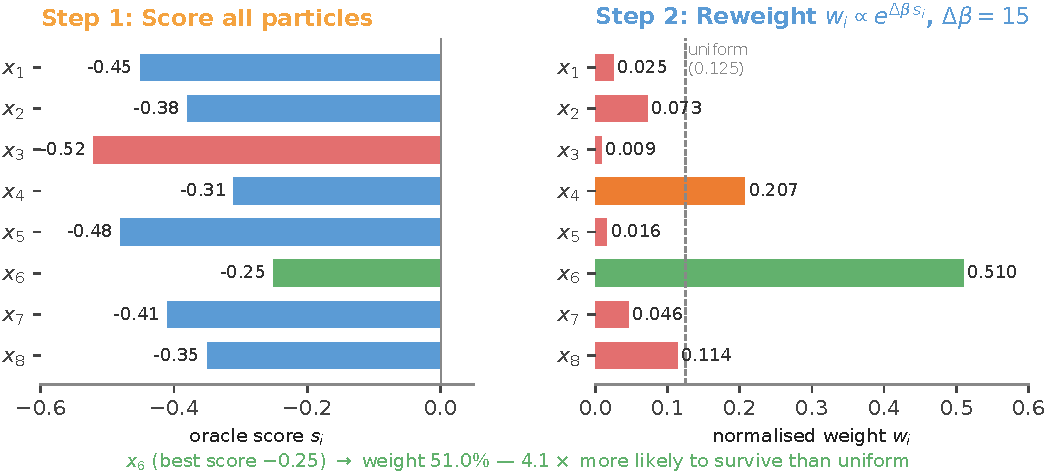
\includegraphics[width=0.95\linewidth]{figures/fig_gpa_walkthrough_score.pdf}
\caption{Score and reweight on the $N\!=\!8$ toy. \textbf{Left:} per-particle oracle scores $s_i$ (best in green: $x_6\!=\!-0.25$; worst in red: $x_3\!=\!-0.52$). \textbf{Right:} normalised weights after the tilt $w_i\!\propto\!\exp(\Delta\beta\,s_i)$ at $\Delta\beta\!=\!15$; uniform $1/N\!=\!0.125$ shown dashed. $x_6$ collects $51.0\%$ of the mass---$4.1\!\times$ the uniform expectation.}
\label{fig:walkthrough-score}
\end{figure}

\subsection{Adapting $\Delta\beta$ via bisection on $\ESS$}

The ESS-adaptive schedule (Lemma~\ref{lem:ess}) chooses $\Delta\beta_t$ so that $\ESS\!\geq\!\alpha N$ \emph{exactly} (not below). With $\alpha\!=\!0.5$, the target is $\ESS_{\rm target}\!=\!4$. Algorithm~\ref{alg:bisect} runs 64 bisection iterations on $[\Delta\beta_{\min}, \Delta\beta_{\max}]\!=\![0,1000]$.

\begin{algorithm}[h]
\caption{Bisection for $\Delta\beta$ given $\ESS$ target}\label{alg:bisect}
\begin{algorithmic}[1]
\State \textbf{Input:} scores $\{r_i\}_{i=1}^N$, target $\tau N$, range $[\Delta\beta_{\min}, \Delta\beta_{\max}]$, max iters $T_{\rm bs}$
\For{$t\!=\!1,\dots,T_{\rm bs}$}
    \State $\Delta\beta_{\rm mid}\!\leftarrow\!(\Delta\beta_{\min}+\Delta\beta_{\max})/2$
    \State $w_i\!\leftarrow\!\exp(\Delta\beta_{\rm mid}\,r_i)/Z$, with $Z\!=\!\sum_j\exp(\Delta\beta_{\rm mid}\,r_j)$
    \State $\ESS\!\leftarrow\!1/\sum_i w_i^2$
    \If{$\ESS > \tau N$} $\Delta\beta_{\min}\!\leftarrow\!\Delta\beta_{\rm mid}$ \Comment{can push harder}
    \Else \;$\Delta\beta_{\max}\!\leftarrow\!\Delta\beta_{\rm mid}$ \Comment{too aggressive}
    \EndIf
\EndFor
\State \textbf{Return:} $\Delta\beta_{\min}$
\end{algorithmic}
\end{algorithm}

For our example, the bisection converges to $\Delta\beta\!\approx\!11.7$, giving $\ESS\!\approx\!4.0\!=\!\alpha N$. The hand-picked $\Delta\beta\!=\!15$ above (which produced $\ESS\!=\!3.08$) was therefore more aggressive than the auto-schedule would choose.

\begin{figure}[h]
\centering
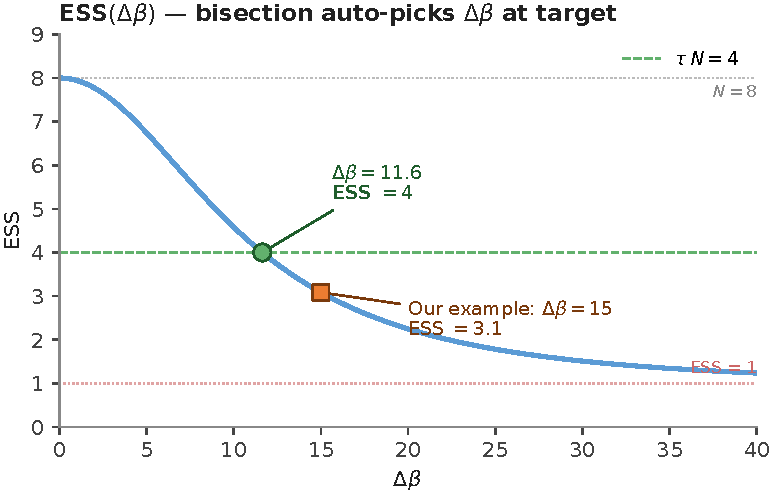
\includegraphics[width=0.78\linewidth]{figures/fig_gpa_walkthrough_ess.pdf}
\caption{$\ESS(\Delta\beta)$ for the $N\!=\!8$ toy oracle scores. The function decreases monotonically from $\ESS\!=\!N$ at $\Delta\beta\!=\!0$ toward $\ESS\!=\!1$ as $\Delta\beta\!\to\!\infty$ (winner-take-all). Bisection finds the unique $\Delta\beta\!=\!11.7$ at which $\ESS$ hits the target $\tau N\!=\!4$ (green dot). The hand-picked $\Delta\beta\!=\!15$ used in the walk-through (orange square) is past the target and so over-collapses the population.}
\label{fig:walkthrough-ess}
\end{figure}

\subsection{Resampling: multinomial vs.\ systematic}

\paragraph{Multinomial.} Draw counts $\!=\!(c_1,\dots,c_N)\!\sim\!\mathrm{Multinomial}(N, w)$. Expected copies per particle are $\E[c_i]\!=\!N\!\cdot\!w_i$, but the realised counts are noisy.

\paragraph{Systematic.} Lay the weights end-to-end as a unit interval $[0,1]$ (segment $i$ has width $w_i$). Drop $N$ pointers at positions $u\!+\!k/N$ for $k\!=\!0,\dots,N\!-\!1$, with $u\!\sim\!\mathrm{Uniform}[0,1/N)$. Particle $i$ receives a number of copies equal to the count of pointers in its segment. This has identical mean to multinomial but lower variance, and is the default in \gpa{}.

For our $N\!=\!8$ example with $u\!=\!0$, the eight pointers at $\{0.000, 0.125, 0.250, 0.375, 0.500, 0.625, 0.750, 0.875\}$ land in segments as follows: $w_2$ (cumulative 0.025--0.098) captures pointer 0.097; $w_4$ (0.107--0.314) captures pointers at 0.125, 0.250; $w_6$ (0.330--0.840) captures pointers at 0.375, 0.500, 0.625, 0.750; $w_8$ (0.886--1.000) captures pointer 0.875. Final copy counts:
\begin{center}
\begin{tabular}{lcccccccc}
\toprule
$i$       & 1 & 2 & 3 & 4 & 5 & 6 & 7 & 8 \\
copies    & 0 & 1 & 0 & 2 & 0 & 4 & 0 & 1 \\
\bottomrule
\end{tabular}
\end{center}
Four particles ($x^1, x^3, x^5, x^7$) are eliminated; $x^6$ is duplicated four times. After resampling, weights reset to $1/N\!=\!0.125$ uniformly.

\begin{figure}[h]
\centering
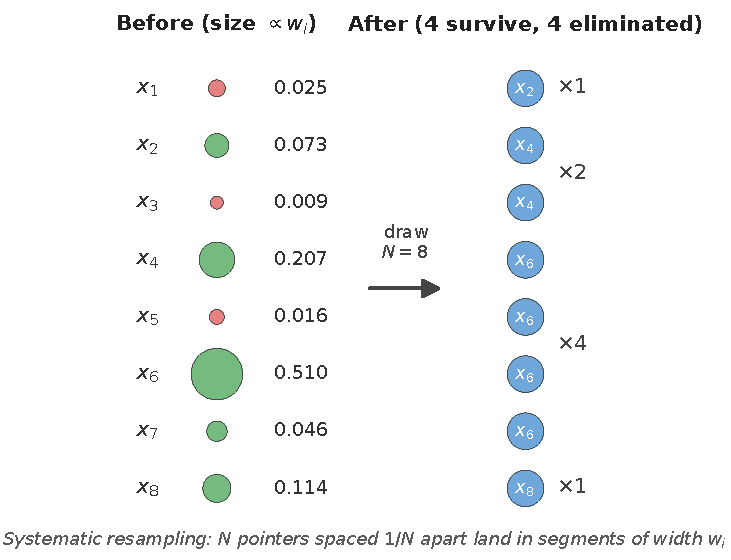
\includegraphics[width=0.85\linewidth]{figures/fig_gpa_walkthrough_resample.pdf}
\caption{Systematic resampling of the $N\!=\!8$ toy. \textbf{Left:} bubble area is proportional to $w_i$; green = retained, red = eliminated by the resampling step. \textbf{Right:} after resampling, all weights reset to $1/N$; $x_6$ now appears four times, $x_4$ twice, $x_2$ and $x_8$ once each. Four particles ($x_1, x_3, x_5, x_7$) are eliminated.}
\label{fig:walkthrough-resample}
\end{figure}

\subsection{Mutation: partial mask + denoise on a length-12 DNA toy}

Each of the eight resampled (now duplicate-rich) particles is independently mutated by $K_\beta$. Concretely, with mask fraction $\mathrm{nf}\!=\!0.25$ ($\!\to\!\lceil 0.25\!\cdot\!12\rceil\!=\!3$ positions on a length-12 sequence):
\begin{center}
\begin{tabular}{ll}
\toprule
\textbf{Step}        & \textbf{Sequence} \\
\midrule
Before (a duplicate of $x^6$)   & \texttt{ACGTATGCACGT} \\
Random mask 3 positions          & \texttt{AC?TA?GC?CGT} \\
Denoise via $p_\theta$           & \texttt{AC\textbf{T}TA\textbf{A}GC\textbf{A}CGT} \\
\midrule
Net edits                         & pos 3: G$\to$T; \, pos 6: T$\to$A; \, pos 9: C$\to$A \\
\bottomrule
\end{tabular}
\end{center}
Two properties this kernel inherits from the pretrained $p_\theta$:
\begin{itemize}
\item \emph{Grammar preservation.} The denoiser sees the unmasked context and proposes tokens consistent with whatever motif/composition rules $p_\theta$ has learned. Random per-position resampling would not.
\item \emph{Diversity restoration.} The four duplicates of $x^6$ each get an \emph{independent} random mask + denoising pass, so they diverge into four distinct child sequences. Without mutation the population would collapse to four identical copies.
\end{itemize}
The mask fraction $\mathrm{nf}$ controls exploration: $\mathrm{nf}\!=\!0.05$ is local search ($\sim\!10$ positions per step on a 200-bp DNA enhancer), $\mathrm{nf}\!=\!0.20$ is large jumps. Section~\ref{sec:results:ablation} reports sensitivity in the practical range.

%-----------------------------------------------------------------------
\section{Hyperparameters}\label{app:hyper}

Table~\ref{tab:hyper-rerd} lists hyperparameters for the SMC-protocol comparison (\drakes{} eval pair); Table~\ref{tab:hyper-ctrldna} lists those for \ctrldna{} comparison (HyenaDNA + gReLU MSE oracles); Table~\ref{tab:hyper-dnacraft} for \dnacraft{} comparison (HyenaDNA/DiMamba + Enformer 50/50). Default values are bolded.

\begin{table}[h]
\caption{Hyperparameters for the SMC-protocol comparison (HepG2 enhancer, MDLM backbone, \drakes{} split-oracle).}
\label{tab:hyper-rerd}
\centering
\small
\begin{tabular}{lll}
\toprule
Parameter & Mean recipe & Spec recipe \\
\midrule
$N$ (population) & 5000 & 5000 \\
$\alpha$ (ESS threshold) & 0.5 & 0.5 \\
$\beta_*$ (target inverse temp) & 200 & 100 \\
$T_{\max}$ (max steps) & 30, hard cap 200 & 30, hard cap 200 \\
nf (mask fraction) & 0.05 & 0.05 \\
DPS gradient strength $\eta$ & 3000 & 3000 \\
$\mathrm{pw}$ (off-target penalty) & 0 & 0.35 \\
GC bio-filter & [0.45, 0.55] & [0.45, 0.55] \\
\bottomrule
\end{tabular}
\end{table}

\begin{table}[h]
\caption{Hyperparameters for \ctrldna{} comparison (Reddy promoters, HyenaDNA backbone, gReLU MSE oracles, universal recipe).}
\label{tab:hyper-ctrldna}
\centering
\small
\begin{tabular}{ll}
\toprule
Parameter & Universal recipe \\
\midrule
$N$ (population) & 10000 \\
$\alpha$ (ESS threshold) & 0.5 \\
$\beta_*$ & 100 \\
$T_{\max}$ (steps) & 60 \\
nf (mask fraction) & 0.05 \\
$K$ (branch factor) & 8 \\
$\mathrm{pw}$ & 0.35 \\
diversity $\lambda$ (conformity) & \textbf{1.0} \\
DPS & off \\
GC bio-filter & off \\
\bottomrule
\end{tabular}
\end{table}

\begin{table}[h]
\caption{Hyperparameters for \dnacraft{} comparison (Gosai 50/50 split, top-128 by MinGap-Eval). C1 = no GC penalty; C3 = soft GC penalty (gct=0.60), no hard bio-filter.}
\label{tab:hyper-dnacraft}
\centering
\small
\begin{tabular}{lll}
\toprule
Parameter & C1 & C3 \\
\midrule
$N$ (population) & 5000 & 5000 \\
$\beta_*$ & 25 & 25 \\
$\mathrm{pw}$ & 0.30 & 0.30 \\
DPS & on & on \\
GC penalty (gct) & --- & 0.60 \\
GC bio-filter & off & off \\
$K$ & 8 & 8 \\
\bottomrule
\end{tabular}
\end{table}

%-----------------------------------------------------------------------
\section{Full GPA-vs-ISM/LEDIDI tables}\label{app:ism_full}

Single-sequence comparison: GPA row = the one sequence in each pool that maximises $\mathrm{AG}-\mathrm{LN}$ (sweet spot: low LN, high held-out AG). Directly comparable to \ism{}/\ledidi{} which are inherently single-sequence.

\begin{table}[h]
\caption{Single-sequence comparison, K562 enhancer, two seeds (uid=181692 natural, uid=50178 random). \gpa{} row = argmax of $\mathrm{AG}-\mathrm{LN}$ within the 5{,}000-seq pool.}
\label{tab:ism_singleseq}
\centering
\small
\begin{tabular}{llrrr}
\toprule
Seed & Method & Edits & LN & AG \\
\midrule
\multirow{4}{*}{uid=181692}
 & \gpa{} (no DPS) uncap   &  96 & 4.97 & \textbf{3.33} \\
 & \gpa{} (+DPS) cap30     &  60 & 6.21 & \textbf{3.47} \\
 & \ism{} gen 115          & 115 & 8.74 & 2.83 \\
 & \ledidi{} t15 $\lambda$=0.05 & 125 & 9.81 & $-$0.22 \\
\midrule
\multirow{4}{*}{uid=50178}
 & \gpa{} (no DPS) cap30   &  60 & 4.71 & 2.75 \\
 & \gpa{} (+DPS) cap30     &  59 & 6.58 & \textbf{3.61} \\
 & \ism{} gen 115          & 115 & 9.58 & 2.92 \\
 & \ledidi{} t15 $\lambda$=0.05 & 105 &11.66 & $-$0.62 \\
\bottomrule
\end{tabular}
\end{table}

\paragraph{Reading the table.}
A single \gpa{} sequence (e.g.\ +DPS cap30 on uid=50178: LN $6.58$, AG $3.61$) beats \ism{} gen 115 on the held-out AG by $+0.69$ at LN $\sim\!3.0$ lower—better held-out activity \emph{and} less reward-hacking. Under any selection rule, \ledidi{} stays AG-negative; not one of its 50 reruns produces an AG-positive sequence.

\paragraph{Apples-to-apples runtime (single H100, K562 enhancer, 5{,}000-sequence pool).}
Table~\ref{tab:ism_runtime} reports wall-time at matched output volume, averaged across the random and natural pools. \gpa{} is fully population-parallel: a single SMC step propagates all 5{,}000 particles together through the diffusion proposal, so the per-particle cost is the GPU-memory chunk \texttt{mutation\_batch\_size=128} amortised over the population. \ism{} is also nominally population-parallel (5{,}000 independent greedy trajectories), but its sequential cost is fixed at 115 generations per seed, and that dominates wall regardless of how memory chunks are batched. \ledidi{} is chunked-sequential by design: 5{,}000 seeds processed in 39 chunks of 128 along the Gumbel-softmax optimisation. The result is $\sim\!9.3\times$ speedup over \ism{} and $\sim\!3.4\times$ speedup over \ledidi{} at identical pool size and identical hardware.

\begin{table}[h]
\caption{Apples-to-apples runtime: single H100, 5{,}000-sequence K562-enhancer pool, averaged across random and natural seed pools. \gpa{} = v3 noDPS recipe (matches Sec.~\ref{sec:results:ism}). Speedup column is $\mathrm{wall}_{\text{baseline}}/\mathrm{wall}_{\gpa{}}$.}
\label{tab:ism_runtime}
\centering
\small
\begin{tabular}{lllr}
\toprule
Method & Wall (5K pool) & Parallelism & Speedup vs.\ \gpa{} \\
\midrule
\textbf{\gpa{}} & \textbf{$\sim\!11.6$ min} & population-parallel (5{,}000 SMC particles) & --- \\
\ledidi{}       & $\sim\!40$ min     & chunked-sequential (39 chunks $\times$ 128 seeds) & $\sim\!3.4\times$ slower \\
\ism{}          & $\sim\!107.5$ min  & population-parallel, but 115 sequential greedy gens & $\sim\!9.3\times$ slower \\
\bottomrule
\end{tabular}
\end{table}

%-----------------------------------------------------------------------
\section{Full DNA-CRAFT tables (GPA-C1 vs GPA-C3)}\label{app:dnacraft_full}

The headline column in Table~\ref{tab:dnacraft} uses GPA-C3 (\texttt{dps\_pw030\_b25\_gct060\_nobio}). This appendix shows the same benchmark with the alternate recipe variant GPA-C1 (\texttt{dps\_pw030\_b25}, no GC penalty), under the matched-output-budget protocol of Table~\ref{tab:dnacraft} (\texttt{by\_pool\_composite} top-64 from \texttt{gpa\_output\_best\_eval.h5}, 3 reps for both variants). Both variants run at $\sim\!3.6$ min/seed (no MCTS) on the MDLM backbone; the only difference is the soft GC-centering term added to C3's DPS gradient.

\paragraph{Recipe decomposition.}
Each token in the recipe name maps to a specific knob in the GPA algorithm of \S\ref{sec:method}, with no other differences between the two variants:
\begin{itemize}
\item \texttt{dps} -- enables the Gumbel-softmax oracle gradient with strength $\eta\!=\!3000$ (\S\ref{sec:method:ext}, ``Gumbel-softmax oracle gradient (DPS)''). This is a biased proposal in the sense of \S\ref{sec:method:ext} and is shared by both C1 and C3, so the C1$\leftrightarrow$C3 contrast does not move along the DPS-bias axis.
\item \texttt{pw030} -- sets the off-target weight $\mathrm{pw}\!=\!0.30$ in the linear fitness of Eq.~\ref{eq:fitness} (\S\ref{sec:method:pw}); the same $0.30$ weights the off-target term inside the DPS gradient as well.
\item \texttt{b25} -- sets the SMC tilt ceiling $\beta_*\!=\!25$. This is below the default range $\beta_*\!\in\!\{100,200\}$ in \S\ref{sec:exp} and is a deliberately gentler tilt that preserves population diversity at some cost in MinGap; both variants share it.
\item \texttt{gct060} \emph{(C3 only)} -- adds a quadratic centering term $-w\,(g(x)-0.60)^2$ to the DPS objective before backpropagation, where $g(x)\!=\!\overline{P(C)+P(G)}$ is the per-position soft-onehot GC fraction and $w\!=\!10$. The penalty rides inside the same Gumbel-softmax gradient that DPS already computes; it is \emph{not} a hard accept/reject filter.
\item \texttt{nobio} -- disables the hard bio-filter (no \texttt{gc\_low}/\texttt{gc\_high} interval gating). All GC discipline in C3 therefore comes from the soft \texttt{gct060} term in the DPS gradient.
\end{itemize}
Both variants additionally use the default branch factor $K\!=\!8$ (\S\ref{sec:method:ext}, Prop.~\ref{prop:K}) and population $N\!=\!5{,}000$ (Table~\ref{tab:dnacraft} caption), so both target $\pi_{\beta_*}^{(K=8)}\!\neq\!\pi_{\beta_*}$ in the sense of Prop.~\ref{prop:K}; the C1$\leftrightarrow$C3 contrast isolates the GC-centering term with $K$, $\beta_*$, $\mathrm{pw}$, $N$, and the DPS bias all held constant.

\begin{table}[h]
\caption{\dnacraft{} benchmark with the GPA-C1 alternate recipe (\texttt{dps\_pw030\_b25}; no GC penalty), reported alongside the headline GPA-C3 (Table~\ref{tab:dnacraft}). Both columns: \texttt{by\_pool\_composite} top-64 from \texttt{gpa\_output\_best\_eval.h5}, mean (std) over 3 reps. Baselines verbatim from \citet{dnacraft2026}.}
\label{tab:dnacraft_full_eval}
\centering
\scriptsize
\begin{tabular}{llcccccccccc}
\toprule
Cell & Metric & SMC & CG & TDS & DRAKES & D3 & Ledidi & Ctrl-DNA & DNA-CRAFT & \gpa{}-C1 & \gpa{}-C3 \\
\midrule
\multirow{4}{*}{HepG2}
 & MinGap   & 1.61 & $-$0.23 & 0.40 & $-$1.40 & 0.05 & 5.77 & \textbf{7.79} & 4.35 & 6.87 & 6.91 \\
 & Motif    & 0.55 & 0.86 & 0.40 & 0.06 & 0.87 & 0.58 & 0.63 & \textbf{0.92} & 0.90 & \textbf{0.92} \\
 & 3-mer    & 0.81 & 0.97 & 0.74 & $-$0.36 & \textbf{0.98} & 0.76 & 0.49 & \textbf{0.98} & 0.95 & 0.95 \\
 & Diversity& 0.83 & \textbf{1.98} & 0.96 & 1.86 & \textbf{1.98} & \textbf{1.98} & 1.90 & \textbf{1.98} & 1.81 & 1.86 \\
\midrule
\multirow{4}{*}{K562}
 & MinGap   & 4.12 & 0.00 & 1.62 & $-$0.20 & 0.18 & 7.66 & \textbf{9.07} & 5.69 & 8.18 & 8.13 \\
 & Motif    & 0.45 & 0.85 & 0.51 & 0.14 & 0.86 & 0.65 & 0.63 & 0.93 & 0.93 & \textbf{0.94} \\
 & 3-mer    & 0.66 & 0.94 & 0.65 & $-$0.35 & 0.96 & 0.69 & 0.41 & \textbf{0.98} & 0.92 & 0.95 \\
 & Diversity& 0.31 & \textbf{1.98} & 0.64 & 1.96 & \textbf{1.98} & \textbf{1.98} & 1.90 & \textbf{1.98} & 1.56 & 1.83 \\
\midrule
\multirow{4}{*}{SK-N-SH}
 & MinGap   & 0.56 & $-$0.28 & 0.19 & 0.09 & $-$0.01 & 3.03 & 3.72 & 3.23 & \textbf{5.07} & 4.98 \\
 & Motif    & 0.52 & 0.86 & 0.48 & 0.23 & 0.84 & 0.38 & 0.48 & 0.88 & 0.89 & \textbf{0.92} \\
 & 3-mer    & 0.78 & 0.95 & 0.72 & $-$0.38 & 0.93 & 0.37 & 0.20 & \textbf{0.97} & 0.87 & 0.94 \\
 & Diversity& 1.27 & \textbf{1.98} & 0.92 & 1.83 & 1.97 & \textbf{1.98} & 1.86 & \textbf{1.98} & 1.59 & 1.86 \\
\bottomrule
\end{tabular}
\end{table}

\paragraph{Reading.}
GPA-C1 and GPA-C3 give nearly tied MinGap and Motif Spearman on every cell (within seed std on most rows). C3 wins Motif on HepG2 / K562 / SK-N-SH ($+0.02$/$+0.01$/$+0.03$) and 3-mer on K562 / SK-N-SH ($+0.03$/$+0.07$). The biggest practical difference is Diversity: the soft GC-centering term in C3's DPS gradient recovers $+0.05$ to $+0.27$ Shannon bits over C1 on every cell, lifting C3 above the Ctrl-DNA Diversity floor on all three cells. The mechanism is indirect: by penalising drift away from $g(x)\!=\!0.60$ at every Gumbel-softmax step, the term blunts the oracle's tendency to push particles toward narrow high-GC modes, which in turn keeps the population spread out in sequence space. C1 wins MinGap on K562 / SK-N-SH ($+0.05$/$+0.09$) but loses across the rest. C3 is the headline because the +Diversity / +Motif / +3-mer trade dominates the small MinGap give-back; C1 is reported as an ablation that isolates the GC-penalty's contribution.

\paragraph{Backbone caveat.}
\dnacraft{}'s reported numbers in Table~\ref{tab:dnacraft} are obtained on a Mamba-style discrete-diffusion (DiMamba) backbone whose code and pretrained checkpoints are not publicly available; the same paper also reports DiMamba-vs-MDLM ablations that show DiMamba contributes additional biological-faithfulness gains. Our \gpa{}-C1 / \gpa{}-C3 numbers are obtained on the publicly available MDLM backbone of \citet{sahoo2024mdlm} and should be read as a lower bound on what \gpa{} would achieve at backbone parity, by Remark~\ref{rem:agnostic}.

%-----------------------------------------------------------------------
\section{Wall-time table}\label{app:wall}

\begin{table}[h]
\caption{Wall time per seed and 5-seed totals (HepG2, identical H100 hardware, identical HyenaDNA backbone). Wall time excludes downstream motif scoring.}
\label{tab:wall}
\centering
\small
\begin{tabular}{lrr}
\toprule
Method & Wall/seed (h) & 5-seed total (GPU-h) \\
\midrule
\ctrldna{} R200 (RL fine-tune) & $43.5\pm 0.8$ & $\sim\!218$ \\
\gpa{} v3 (K=8, no diversity)  & $3.97\pm 0.59$ & 19.8 \\
\gpa{} v4 (K=8 + rejuvenation) & $2.17\pm 0.22$ & 10.8 \\
\gpa{} v5 (K=8 + diversity)    & $\mathbf{2.22\pm 0.52}$ & $\mathbf{11.1}$ \\
\bottomrule
\end{tabular}
\end{table}

%-----------------------------------------------------------------------
\section{DPS gradient ablation}\label{app:dps_ablation}

Population annealing alone (no DPS) already beats single-chain refinement baselines; DPS gradient is a multiplicative enhancement.

\begin{table}[h]
\caption{DPS gradient ablation on Gosai HepG2.}
\label{tab:dps_ablation}
\centering
\small
\begin{tabular}{llrrr}
\toprule
Track & Metric & \gpa{}-only & \gpa{}+DPS & $\Delta$(DPS) \\
\midrule
Mean & $H_{\mathrm{eval}}$ & $8.73\pm 0.50$ & $\mathbf{10.06\pm 0.19}$ & $+1.33$ \\
Mean & Spec & 1.58 & 3.06 & $+1.48$ \\
Spec & $H_{\mathrm{eval}}$ & $8.28\pm 0.12$ & $9.35\pm 0.20$ & $+1.07$ \\
Spec & Spec & $6.11\pm 1.45$ & $\mathbf{7.61\pm 0.25}$ & $+1.50$ \\
\bottomrule
\end{tabular}
\end{table}

%-----------------------------------------------------------------------
\section{Naturalness audit}\label{app:naturalness}

\begin{table}[h]
\caption{Naturalness audit (HepG2 top-128). \gpa{} produces bio-plausible sequences by construction; \ctrldna{} reward-hacks to non-biological space.}
\label{tab:nat}
\centering
\small
\begin{tabular}{lrrr}
\toprule
Metric & Real (Gosai) & \gpa{} & \ctrldna{} \\
\midrule
GC mean & 0.44 & 0.41 & 0.45 \\
\textbf{bio\_pass\_rate} & 0.51 & $\mathbf{1.00}$ & $\mathbf{0.05}$ \\
max homopolymer & 5.4 & 5.1 & $\mathbf{20.9}$ \\
$k$=3 Pearson & 1.0 & 0.61 & 0.39 \\
HNF1A enrichment & $0\times$ & $10\,040\times$ & $7\,812\times$ \\
\bottomrule
\end{tabular}
\end{table}

\begin{figure}[h]
\centering
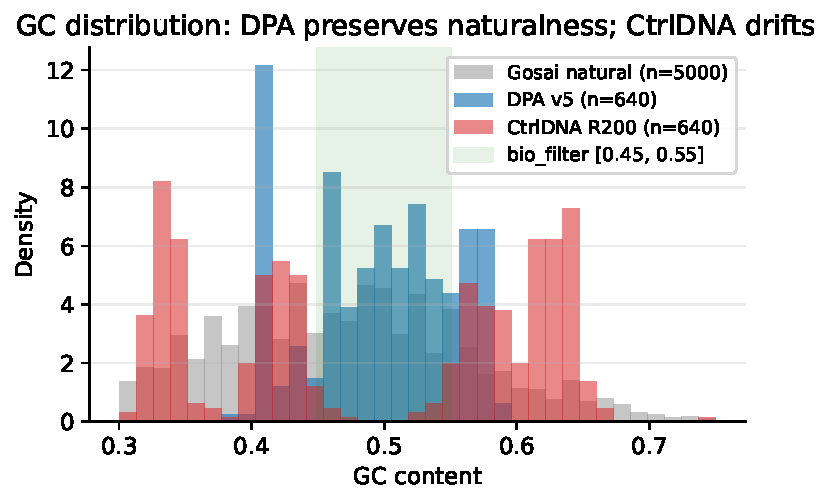
\includegraphics[width=0.6\linewidth]{figures/fig2_gc.pdf}
\caption{GC distribution comparison on HepG2 top-128 sequences. \gpa{} (blue) clusters near the lower edge of the bio-filter (45\%) but stays within the natural Gosai range (gray); \ctrldna{} (red) drifts widely, with a heavy tail of low- and high-GC sequences and a substantial fraction outside the natural distribution.}
\label{fig:gc}
\end{figure}

%-----------------------------------------------------------------------
\section{Extreme specificity}\label{app:extreme}

Pushing $\mathrm{pw}$ beyond the canonical $0.35$ trades $H_{\mathrm{eval}}$ for higher specificity until both off-targets fall below baseline (Table~\ref{tab:extreme}).

\begin{table}[h]
\caption{Extreme-specificity extension on Gosai HepG2 (single run each, $N\!=\!5000$).}
\label{tab:extreme}
\centering
\small
\begin{tabular}{rrrrr}
\toprule
$\mathrm{pw}$ & $H_{\mathrm{eval}}$ & $K_{\mathrm{eval}}$ & $S_{\mathrm{eval}}$ & $H{>}8 \wedge K{<}0 \wedge S{<}0$ \\
\midrule
0.35 & 9.65 & 2.15 &  1.10 & 0 \\
0.50 & 9.54 & 1.96 &  0.63 & 0 \\
0.70 & 8.73 & 1.52 &  0.35 & 0 \\
1.00 & 8.57 & 0.69 & $-$0.48 & 26 \\
1.50 & $\mathbf{8.44}$ & 0.55 & $\mathbf{-0.66}$ & $\mathbf{54}$ \\
\bottomrule
\end{tabular}
\end{table}

\paragraph{Beta trajectory.}
Figure~\ref{fig:beta} shows a representative ESS-adaptive $\beta$ trajectory and the population-mean reward over SMC steps for a HepG2 run.

\begin{figure}[h]
\centering
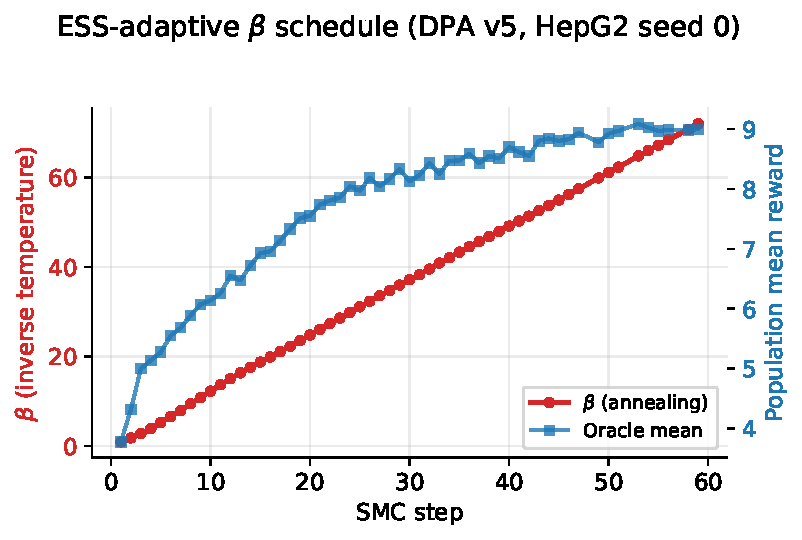
\includegraphics[width=0.6\linewidth]{figures/fig4_beta_traj.pdf}
\caption{Representative \gpa{} run trajectory (HepG2, seed 0). Red trace: ESS-adaptive $\beta$ schedule rises through the annealing path. Blue trace: population mean reward grows monotonically toward saturation as $\beta$ increases.}
\label{fig:beta}
\end{figure}

%-----------------------------------------------------------------------
\section{Negative result: APF correction for $\epsilon$-greedy $K$-branching}\label{app:apf}

A natural attempt to recover Shannon under $K$-branching is to soften the argmax with $\epsilon$-greedy ($\tau\!>\!0$ softmax over the $K$ siblings) and apply the auxiliary-particle-filter weight correction \citep{pittshephard1999}:
\[
w_{\mathrm{new}} = w_{\mathrm{old}}\big/p_\tau(\mathrm{winner}),\qquad p_\tau(j)=\exp(r_j/\tau)\big/\sum_m\exp(r_m/\tau).
\]
Compute the expectation:
\[
\E[w_{\mathrm{new}}\,\varphi(x_{\mathrm{winner}})] = \E_{x_{1:K}\sim q}\!\!\left[\sum_{j=1}^K \frac{\exp(r_j/\tau)}{\sum_m\exp(r_m/\tau)}\cdot\frac{\sum_m\exp(r_m/\tau)}{K\exp(r_j/\tau)}\,\varphi(x_j)\right]=\frac{1}{K}\sum_j \E_q[\varphi(x_j)],
\]
i.e.\ the corrected estimator is equivalent to a single-child sample. The $K$ siblings collapse and the effective-$\beta$ boost vanishes. Empirically, on a synthetic linear reward $r(x)\!=\!3x$ with $q$ uniform on $[0,1]$ (200K Monte-Carlo trials):
\begin{center}
\small
\begin{tabular}{lrrr}
\toprule
Variant & $\E[x]$ & $\mathrm{Var}[x]$ & ESS \\
\midrule
$K=1$ no selection                & 0.5000 & 0.0833 & 100.0\% \\
$K=8$ argmax (no correction)      & 0.8887 & 0.0099 & 100.0\% \\
$K=8$ softmax $\tau\!=\!0.3$ (no corr.) & 0.8445 & 0.0180 & 100.0\% \\
\textbf{$K=8$ softmax $\tau\!=\!0.3$ + APF} & 0.4880 & 0.0874 & 0.4\% \\
$K=8$ softmax $\tau\!=\!1.0$ + APF & 0.5009 & 0.0829 & 53.1\% \\
\bottomrule
\end{tabular}
\end{center}
ESS collapses at low $\tau$ and the corrected mean/variance reproduces $K=1$. We therefore do \emph{not} use APF correction for production runs and report only argmax $K$-branching. K-annealing schedules and waste-free SMC \citep{dau2022wastefree} remain valid theoretical alternatives, deferred to future work.

%-----------------------------------------------------------------------
\section{Negative result: post-hoc Metropolis tempering}\label{app:posthoc}

Another natural Shannon-rescue move is to load the concentrated argmax-$K$ pool and run Metropolis–Hastings at lower $\beta'$ to spread the population. We tested this on the K562 promoter pool (50 MH steps, nf=0.05, HyenaDNA proposal):

\begin{center}
\small
\begin{tabular}{rrrrr}
\toprule
$\beta'$ & accept rate & $\Delta$comp & $\Delta$tgt & $\Delta H$ \\
\midrule
25 &  3.4\% & $+0.02$ & $-0.06$ & $+0.05$ \\
12 &  6.5\% & $-0.15$ & $-0.27$ & $+0.10$ \\
 6 & 13.1\% & $-0.68$ & $-0.77$ & $+0.21$ \\
 3 & 29.1\% & $-2.12$ & $-2.22$ & $+0.39$ \\
 1 & 73.7\% & $-4.71$ & $-5.35$ & $+0.61$ \\
\bottomrule
\end{tabular}
\end{center}
The Pareto slope is $\sim\!3\!-\!5$ target units per $0.1$ nat of Shannon, far too steep for the diversity gap to \dnacraft{}/\ctrldna{} K562 ($\sim\!0.5$ nat) to be closed without erasing the target advantage. Increasing chain length or shrinking nf does not change the local-neighborhood geometry. The honest reading: under sharply peaked oracles, the activity–diversity tension is in the reward landscape, not the sampler.

%-----------------------------------------------------------------------
\section{GC distribution and floor-hugging}\label{app:gc}

Even with the bio-filter $\mathrm{GC}\!\in\![0.45,0.55]$, $60\!-\!75\%$ of \gpa{} top-128 sequences cluster at the lower bound. Two facts:
\begin{enumerate}
\item This is a property of the \emph{masked-diffusion proposal} at low noise fraction. At $\mathrm{nf}\!=\!0.20$ the bias inverts toward the upper bound (GC $\approx\!0.54$); the crossover occurs near $\mathrm{nf}\!\approx\!0.16\!-\!0.17$.
\item The eval oracle is GC-agnostic: at both $\mathrm{nf}$ extremes, top-128 oracle scores are comparable. The GC bias arises from $p_\theta$, not from the reward signal.
\end{enumerate}
Three mitigations were tested with mixed success: (i) GC-aware DPS gradient (\verb|gc_dps_weight|) reduces floor-hugging from $61.5\%$ to $55.0\%$ at $-0.09$ $H_{\mathrm{eval}}$ cost; (ii) narrow $1\%$ GC bands achieve uniform GC by construction at $-0.25$ $H_{\mathrm{eval}}$; (iii) stratified resampling within $2\%$ GC bins \citep{verge2015island} achieves balanced coverage at $-0.50$ to $-1.0$ $H_{\mathrm{eval}}$. We report all three options in the codebase but use the unmitigated baseline in the headline tables for fair comparison with peer methods.

%-----------------------------------------------------------------------
\section{Ctrl-DNA enhancer comparison (V7 main + V5/V8 ablations)}\label{app:ctrldna_enhancer}

This appendix gives the dedicated \ctrldna{}-vs-\gpa{} enhancer comparison referenced in \S\ref{sec:results:promoter}. Same Gosai 50/50 split as the \dnacraft{} benchmark, top-128 selection per cell, 5 \gpa{} seeds. The headline GPA recipe is V7 (universal: $K\!=\!8$, diversity $\lambda\!=\!1.0$); V8a, V8b (alternative pairwise-suppression formulations) and V5 (the previous default with $\lambda\!=\!0.2$) are ablations.

\begin{table}[h]
\caption{Ctrl-DNA vs.\ \gpa{} on Gosai HepG2/K562/SKNSH enhancers (5 seeds; mean (std)). Headline = V7 universal recipe; V8a (log\_ratio + pw=1.0), V8b (linear + pw=1.0) and V5 ($\lambda\!=\!0.2$) are ablations of the diversity / pairwise-suppression knob. \texttt{target\_raw} = mean target oracle score; \texttt{ΔR} = normalised target minus mean off-target; \texttt{shannon} = per-position entropy; \texttt{motif\_corr} = FIMO Pearson against per-cell real reference.}
\label{tab:ctrldna_enhancer}
\centering
\footnotesize
\setlength{\tabcolsep}{4pt}
\begin{tabular}{llrrrr}
\toprule
Cell & Method & target\_raw $\uparrow$ & ΔR $\uparrow$ & shannon $\uparrow$ & motif\_corr $\uparrow$ \\
\midrule
\multirow{5}{*}{HepG2}
 & \ctrldna{} R200             & 5.32 (0.65) & 0.48 (0.10) & 1.65 (0.14) & \textbf{0.29} (0.16) \\
 & \gpa{} V5 ($K\!=\!8, \lambda\!=\!0.2$) & 9.86 (0.10) & 0.85 (0.01) & 1.49 (0.03) & 0.19 (0.03) \\
 & \gpa{} V7 ($K\!=\!8, \lambda\!=\!1.0$) & \textbf{9.90} (0.12) & 0.84 (0.02) & 1.59 (0.11) & 0.20 (0.02) \\
 & \gpa{} V8a (log\_ratio, pw=1.0) & 6.61 (0.04) & 0.68 (0.01) & \textbf{1.93} (0.00) & 0.15 (0.02) \\
 & \gpa{} V8b (linear, pw=1.0) & 9.51 (0.10) & \textbf{0.93} (0.02) & 1.70 (0.11) & 0.10 (0.04) \\
\midrule
\multirow{5}{*}{K562}
 & \ctrldna{} R200             & \textbf{9.99} (1.52) & \textbf{0.77} (0.14) & 1.60 (0.15) & 0.24 (0.07) \\
 & \gpa{} V5 ($K\!=\!8, \lambda\!=\!0.2$) & 8.82 (0.13) & 0.34 (0.00) & 1.43 (0.09) & \textbf{0.26} (0.02) \\
 & \gpa{} V7 ($K\!=\!8, \lambda\!=\!1.0$) & 8.83 (0.12) & 0.32 (0.01) & 1.65 (0.02) & 0.24 (0.02) \\
 & \gpa{} V8a (log\_ratio, pw=1.0) & 6.48 (0.03) & 0.39 (0.01) & \textbf{1.94} (0.01) & 0.24 (0.01) \\
 & \gpa{} V8b (linear, pw=1.0) & 8.15 (0.04) & 0.41 (0.01) & 1.68 (0.02) & 0.25 (0.02) \\
\midrule
\multirow{5}{*}{SK-N-SH}
 & \ctrldna{} R200             & 9.93 (1.13) & \textbf{0.71} (0.10) & 1.63 (0.17) & \textbf{0.23} (0.10) \\
 & \gpa{} V5 ($K\!=\!8, \lambda\!=\!0.2$) & \textbf{14.33} (0.20) & 0.10 (0.01) & 1.49 (0.04) & \textbf{0.23} (0.01) \\
 & \gpa{} V7 ($K\!=\!8, \lambda\!=\!1.0$) & 14.17 (0.18) & 0.10 (0.00) & 1.63 (0.04) & 0.20 (0.01) \\
 & \gpa{} V8a (log\_ratio, pw=1.0) & 6.29 (0.08) & 0.22 (0.01) & \textbf{1.91} (0.01) & 0.15 (0.01) \\
 & \gpa{} V8b (linear, pw=1.0) & 8.26 (0.15) & 0.29 (0.03) & 1.74 (0.05) & 0.10 (0.01) \\
\bottomrule
\end{tabular}
\end{table}

\paragraph{Headlines.}
\gpa{} V7 (the universal recipe) wins target\_raw on HepG2 and SK-N-SH ($+4.58$ and $+4.24$ over \ctrldna{}), and is competitive on K562 within $\sim$1 std. \ctrldna{} retains a ΔR (specificity) edge on K562 and SK-N-SH at the cost of $\sim$50\% lower target activity on HepG2/SK-N-SH and high seed-to-seed variance ($\pm 1.13$--$1.52$). The V7 vs.\ V5 comparison shows the diversity-$\lambda$ bump (from $0.2$ to $1.0$) buys $+0.10$--$0.22$ shannon on every cell at zero target cost, isolating the population-conformity penalty as a strict Pareto improvement. V8a/V8b are alternative pairwise-suppression formulations: V8a (log-ratio reward, pw=1.0) achieves the tightest shannon ($1.91$--$1.94$, near uniform) but at substantial target cost; V8b (linear, pw=1.0) recovers HepG2/K562 target while maximising HepG2 ΔR. The four GPA variants together trace a Pareto front in (target, shannon, motif) space at fixed inference cost---one knob per recipe, no retraining.

%-----------------------------------------------------------------------
\section{DNA-CRAFT $K$ and $i$ scaling sweeps (UCB-MCTS variant)}\label{app:ucb_scaling}

\paragraph{Why MCTS at all.}
DNA-CRAFT replaces the SMC population with a single depth-bounded Monte Carlo Tree Search loop on a DiMamba diffusion backbone, and shows that this delivers state-of-the-art motif and 3-mer grammar fidelity on the Gosai enhancer benchmark (Table~\ref{tab:dnacraft}). The mechanism that delivers their grammar bar is plausible on its face: tree search amortises the cost of choosing the right next mutation by replaying the same scoring oracle across multiple competing children before committing—a strictly more informed proposal than picking the first child that scores well. \gpa{}'s standard $K$-branch is a depth-1 special case of this idea: try $K$ candidates from the proposal and keep the best (Sec.~\ref{sec:method:ext}). It is natural to ask whether the same \emph{deeper} planning that powers \dnacraft{}'s grammar—expanding the best leaves over multiple iterations rather than just one---closes \gpa{}'s residual gap to \dnacraft{} on motif/3-mer correlation. The \texttt{ucb\_stacked} variant exists to test exactly that question.

\paragraph{What \texttt{ucb\_stacked} does, step by step.}
At every SMC mutation step, each particle $x_t^{(j)}$ becomes the root of an independent Monte Carlo tree. We then run $i$ iterations on that tree, where each iteration follows the standard four-phase MCTS-with-UCB1 loop \citep[``UCT'';][]{kocsis2006uct}:
\begin{enumerate}
\item \emph{Selection.} Traverse from the root to a leaf by greedily picking, at each internal node $v$ with already-expanded children $\{a\}$, the child that maximises the UCB1 score \citep{auer2002ucb,kocsis2006uct}
\begin{equation}\label{eq:ucb1}
    \mathrm{UCB1}(a) \;=\; \bar{Q}(a) \;+\; c\sqrt{\frac{\ln n(v)}{n(a)}},
\end{equation}
where $\bar{Q}(a)\!\in\![0,1]$ is the mean (range-normalised) reward backed up through child $a$, $n(a)$ is the visit count of $a$, $n(v)\!=\!\sum_a n(a)$ is the parent visit count, and $c\!=\!\sqrt{2}$ is the standard exploration constant. The first term exploits children with high empirical value; the second term explores low-visit children with a $\sqrt{\log n / n(a)}$ confidence radius. Together this is the canonical bandit rule of \citet{auer2002ucb} for stochastic multi-armed bandits, and \citet{kocsis2006uct} show that applying it node-wise inside a tree (UCT) inherits the same $\mathcal{O}(\log n)$ regret bound at each node. Children with $n(a)\!=\!0$ are tried first by convention so the second term remains well-defined.
\item \emph{Expansion.} Apply \gpa{}'s standard $K$-branch operator at the selected leaf: draw $K\!=\!8$ children using partial-mask$\circ$denoise + DPS (the same operator the no-MCTS \gpa{} would use as its mutation kernel).
\item \emph{Evaluation.} Score each new child under the eval-side reward.
\item \emph{Backpropagation.} Update visit counts $n(\cdot)$ and value estimates $\bar{Q}(\cdot)$ along the path from each new child up to the root, so the next iteration's UCB1 selection (Eq.~\ref{eq:ucb1}) uses fresh statistics.
\end{enumerate}
We bound the tree depth at $d\!=\!2$, so the planner looks at most two mutation steps ahead. After $i$ iterations the tree has at most $1\!+\!i\!\cdot\!K$ nodes; the mutated state for $x_t^{(j)}$ is the highest-reward leaf in that tree. The SMC step then proceeds as usual: the new particle states are importance-weighted at the next $\beta$, resampled if $\ESS$ degenerates, and the loop continues.

\paragraph{Connection to \dnacraft{}.}
The four-step loop (UCB selection $\to$ $K$-fold expansion $\to$ scoring $\to$ reward backprop) is identical in shape to \dnacraft{}'s tree search. What differs is the \emph{scope} of where the tree sits and how it is consumed:
\begin{itemize}
\item \dnacraft{} runs \emph{one} MCTS for the whole design problem: $N_{\mathrm{iter}}\!=\!64$ iterations, $M\!=\!128$ children per expansion, full leaf-to-clean rollouts. Their MinGap-Set archive accumulates the best $N_{\max}\!=\!64$ leaves seen during the run, and that archive is the output (no SMC, no population).
\item \texttt{ucb\_stacked} runs \emph{many} MCTSs: one per particle, per SMC step. Each tree is run for $i\!\in\!\{12,18,24,36\}$ iterations with $K\!=\!8$ children per expansion at depth $d\!=\!2$, no full rollouts (we score after one denoising step). The output is the SMC population at the final $\beta$, exactly as in standard \gpa{}; the trees are only the per-particle mutation kernel.
\end{itemize}
``Stacked'' refers to the layering: MCTS sits \emph{on top of} the $K$-branch+DPS proposal in the SMC inner loop. The $K$-branch supplies the unit of expansion; UCB1+depth-2 lookahead is the planner that decides which leaf is worth expanding next. In effect, \texttt{ucb\_stacked} is a way to ask: does \dnacraft{}'s planning shape, used as a mutation kernel inside SMC, give us the same grammar advantages \dnacraft{} reports as the entire search?

\paragraph{Cost.}
Each \texttt{ucb\_stacked} mutation step performs $1\!+\!i\!\cdot\!K$ scoring calls per particle (vs.\ standard \gpa{}'s 8). At our default $K\!=\!8, i\!=\!18$ this is $145$ scoring calls per particle per step---roughly $18\!\times$ the standard \gpa{} mutation budget. The wallclock overhead is sub-linear in both axes (we report the empirical scaling laws below); for the $i\!=\!18$ headline configuration this works out to $\sim\!7\!\times$ the standard \gpa{}-C3 wallclock per seed.

\paragraph{What the tables below show.}
The two sweeps below sit on K562 and fix one axis at the pilot value while sweeping the other ($K\!=\!8$ for the $i$-sweep, $i\!=\!12$ for the $K$-sweep), at depth $d\!=\!2$ throughout. Wallclock is per seed on a single H100; all metrics are reported under the matched-output-budget protocol of Table~\ref{tab:dnacraft} (\texttt{by\_pool\_composite} top-64 from \texttt{gpa\_output\_best\_eval.h5}). Both sweeps include the standard $K\!=\!8, i\!=\!12$ pilot anchor (5 seeds) for cross-reference.

\begin{table}[h]
\caption{DNA-CRAFT $i$-axis sweep (K562, $K\!=\!8$, $d\!=\!2$). \texttt{by\_pool\_composite} top-64. 5 seeds for $i\!\in\!\{12,18\}$, 2 seeds for $i\!\in\!\{24,36\}$.}
\label{tab:ucb_i_sweep}
\centering
\small
\begin{tabular}{rrrrrrr}
\toprule
$i$ & $n$ & wall (min) & MinGap & Motif & 3-mer & Diversity \\
\midrule
12 & 5 & 31.35 (3.62) & $+$8.066 (0.063) & 0.940 (0.004) & 0.945 (0.023) & 1.903 (0.022) \\
18 & 5 & 32.26 (0.62) & $+$8.115 (0.013) & 0.942 (0.003) & 0.961 (0.003) & 1.926 (0.027) \\
24 & 2 & 37.07 (4.08) & $+$8.153 (0.075) & 0.940 (0.002) & 0.968 (0.003) & 1.941 (0.012) \\
36 & 2 & 46.60 (3.23) & $+$8.015 (0.001) & 0.941 (0.003) & 0.965 (0.002) & 1.937 (0.014) \\
\bottomrule
\end{tabular}
\end{table}

\begin{table}[h]
\caption{DNA-CRAFT $K$-axis sweep (K562, $i\!=\!12$, $d\!=\!2$). \texttt{by\_pool\_composite} top-64. 5 seeds for $K\!=\!8$ (pilot anchor), 2 seeds for $K\!\in\!\{16,24,32\}$.}
\label{tab:ucb_K_sweep}
\centering
\small
\begin{tabular}{rrrrrrr}
\toprule
$K$ & $n$ & wall (min) & MinGap & Motif & 3-mer & Diversity \\
\midrule
 8 & 5 & 31.35 (3.62) & $+$8.066 (0.063) & 0.940 (0.004) & 0.945 (0.023) & 1.903 (0.022) \\
16 & 2 & 49.39 (6.64) & $+$8.124 (0.108) & 0.939 (0.002) & 0.959 (0.008) & 1.898 (0.043) \\
24 & 2 & 69.00 (13.13) & $+$8.070 (0.016) & 0.942 (0.004) & 0.953 (0.007) & 1.935 (0.008) \\
32 & 2 & 77.40 (4.31) & $+$8.022 (0.103) & 0.936 (0.000) & 0.953 (0.002) & 1.907 (0.045) \\
\bottomrule
\end{tabular}
\end{table}

\paragraph{Reading.}
Wallclock is sub-linear in both axes ($\mathrm{wall}\propto i^{0.369}$, $R^2\!=\!0.91$; $\mathrm{wall}\propto K^{0.672}$, $R^2\!=\!0.99$): MCTS-rollout batching and K-branch parallelisation amortise cost. Under the matched-output-budget pool-composite selection, MinGap is saturated across the full $i$ and $K$ sweeps (range $8.02$--$8.15$, within seed std on every row); Motif and Diversity are also flat ($\Delta < 0.01$ across $i$, $\Delta < 0.04$ across $K$); only 3-mer Pearson shows a mild gain with $i$ ($+0.020$ from $i\!=\!12$ to $i\!=\!24$). UCB-MCTS planning therefore buys negligible additional metric gain over the standard \gpa{}-C3 headline at substantial wallclock overhead, which is why C3 (no MCTS) is the headline column in Table~\ref{tab:dnacraft} and \texttt{ucb\_stacked} is reported here only as an optional variant.

%-----------------------------------------------------------------------
\section{Population-size ($N$) ablation}\label{app:n_sweep}

The headline GPA-C3 numbers in Table~\ref{tab:dnacraft} use the standard $N\!=\!5{,}000$ SMC particle population. SMC theory predicts that the empirical distribution converges to the reward-tilted target at the parametric rate $\mathcal{O}(1/\sqrt{N})$ (Theorem~\ref{thm:smc-app}); the population-as-budget reading in \S\ref{sec:method:smc-recap} predicts \emph{monotonic improvement of every reported metric with growing $N$}. We test this directly: holding the C3 recipe and the matched-output-budget selection rule (\texttt{by\_pool\_composite} top-64) fixed, sweep $N\!\in\!\{128, 500, 1000, 2500, 5000, 10000, 20000\}$ across all three cells of the \dnacraft{} enhancer benchmark, 5 SMC seeds per $(N, \text{cell})$ pair.

\begin{table}[h]
\caption{$N$-axis ablation on the \dnacraft{} enhancer benchmark; GPA-C3 (no MCTS), \texttt{by\_pool\_composite} top-64 from \texttt{gpa\_output\_best\_eval.h5}. Mean (std) over 5 SMC seeds. Every metric improves monotonically with $N$ on every cell, validating the population-as-budget framing of \S\ref{sec:method:smc-recap}.}
\label{tab:n_sweep}
\centering
\small
\begin{tabular}{rrrrr}
\toprule
$N$ & MinGap $\uparrow$ & Motif $\uparrow$ & 3-mer $\uparrow$ & Diversity $\uparrow$ \\
\midrule
\multicolumn{5}{l}{\emph{HepG2}} \\
   128 & 6.052 (0.087) & 0.829 (0.036) & 0.757 (0.084) & 1.415 (0.101) \\
   500 & 6.559 (0.153) & 0.884 (0.022) & 0.843 (0.070) & 1.600 (0.167) \\
 1{,}000 & 6.677 (0.130) & 0.895 (0.008) & 0.923 (0.021) & 1.725 (0.104) \\
 2{,}500 & 6.788 (0.129) & 0.912 (0.005) & 0.938 (0.024) & 1.845 (0.029) \\
 5{,}000 & 6.962 (0.076) & 0.915 (0.006) & 0.952 (0.013) & 1.870 (0.056) \\
10{,}000 & 7.013 (0.189) & 0.920 (0.003) & 0.968 (0.005) & 1.908 (0.014) \\
20{,}000 & \textbf{7.081} (0.149) & \textbf{0.928} (0.006) & \textbf{0.972} (0.004) & \textbf{1.912} (0.020) \\
\midrule
\multicolumn{5}{l}{\emph{K562}} \\
   128 & 7.236 (0.160) & 0.871 (0.012) & 0.774 (0.104) & 1.515 (0.120) \\
   500 & 7.709 (0.175) & 0.915 (0.011) & 0.863 (0.044) & 1.677 (0.129) \\
 1{,}000 & 7.968 (0.083) & 0.933 (0.008) & 0.912 (0.106) & 1.813 (0.070) \\
 2{,}500 & 7.995 (0.082) & 0.939 (0.005) & 0.951 (0.017) & 1.821 (0.065) \\
 5{,}000 & 8.193 (0.086) & 0.942 (0.005) & 0.960 (0.010) & 1.893 (0.042) \\
10{,}000 & 8.230 (0.118) & 0.946 (0.004) & 0.965 (0.007) & 1.919 (0.014) \\
20{,}000 & \textbf{8.313} (0.060) & \textbf{0.952} (0.004) & \textbf{0.977} (0.005) & \textbf{1.936} (0.021) \\
\midrule
\multicolumn{5}{l}{\emph{SK-N-SH}} \\
   128 & 2.230 (0.347) & 0.807 (0.028) & 0.672 (0.081) & 1.384 (0.067) \\
   500 & 4.149 (0.470) & 0.887 (0.011) & 0.844 (0.068) & 1.588 (0.128) \\
 1{,}000 & 4.388 (0.282) & 0.899 (0.009) & 0.901 (0.021) & 1.783 (0.049) \\
 2{,}500 & 4.841 (0.062) & 0.908 (0.010) & 0.923 (0.015) & 1.852 (0.017) \\
 5{,}000 & 4.980 (0.079) & 0.919 (0.004) & 0.937 (0.007) & 1.867 (0.042) \\
10{,}000 & 5.054 (0.077) & 0.918 (0.006) & 0.934 (0.022) & 1.892 (0.028) \\
20{,}000 & \textbf{5.209} (0.037) & \textbf{0.926} (0.003) & \textbf{0.946} (0.011) & \textbf{1.917} (0.028) \\
\bottomrule
\end{tabular}
\end{table}

\paragraph{Reading.}
Every metric is monotone-increasing in $N$ on every cell, validating the SMC convergence framing. The 128$\to$20{,}000 range covers $\sim$2.2 orders of magnitude in particle count and yields large absolute improvements: MinGap $+1.0$ to $+3.0$ across cells, Motif Spearman $+0.08$ to $+0.12$, 3-mer Pearson $+0.20$ to $+0.27$, Shannon $+0.42$ to $+0.53$ bits. The headline $N\!=\!5{,}000$ row sits near the elbow on every metric: at $5{,}000\!\to\!20{,}000$ the marginal gain is small (Motif $+0.013$, 3-mer $+0.020$, MinGap $+0.20$, Shannon $+0.04$ averaged across cells), so the headline represents a near-saturated operating point at $\sim$0.043~sec/design. Larger $N$ keeps paying off but at a diminishing rate, consistent with the parametric-$\sqrt{N}$ slope predicted by Theorem~\ref{thm:smc-app}. All runs use the standard GPA-C3 recipe (\texttt{dps\_pw030\_b25\_gct060\_nobio}; $K\!=\!8$ K-branch; no MCTS) on the MDLM backbone, exactly as Table~\ref{tab:dnacraft}; the only knob varied is the SMC particle count $N$.

%-----------------------------------------------------------------------
\section{Per-cell complete tables}\label{app:full_tables}

CSVs for all completed runs across all recipes for each cell are provided as supplementary code. We refrain from reproducing them here; the headline rows in Tables~\ref{tab:dnacraft},~\ref{tab:promoter} reflect the unified-recipe candidates.
 from main.tex (after \appendix)

%-----------------------------------------------------------------------
\section{Theoretical statements and proofs}\label{app:theory}

This appendix is the formal counterpart to Sec.~\ref{sec:method:theory}. Each subsection takes one of the practical knobs that show up in the algorithm—the ESS-adaptive temperature, the order-statistic branch factor $K$, the off-target penalty weight $\mathrm{pw}$—and answers the same question for it: \emph{what is GPA actually sampling, and at what rate?} We state the result, give the proof or proof sketch, and then pause to translate the result back into something operational—what the assumption costs in practice, what number to look at in the experimental section to see the result land, and where the assumption can be expected to bend.

Throughout, $p_\theta$ is a pretrained discrete-diffusion model on the finite vocabulary $\Sigma$, $r:\mathcal{X}\!\to\!\R$ is a bounded reward, and $K_\beta$ is the Markov mutation kernel obtained by partial-mask$\circ$denoise (Section~\ref{sec:method:core}). The reward-tilted target the sampler is chasing is $\pi_\beta(x)\propto p_\theta(x)\exp(\beta\,r(x))$.

%-----------------------------------------------------------------------
\subsection{Convergence of the base \gpa{} algorithm}\label{app:smc}

\paragraph{What we want.}
We want a guarantee that as the population grows, GPA's weighted empirical average over the particles converges to the population mean of any bounded statistic under $\pi_{\beta_*}$. This is the formal counterpart of the population-as-budget claim in the introduction (Sec.~\ref{sec:method:smc-recap}): more particles $=$ better samples from the reward-tilted target, with a parametric rate that we can quote.

\paragraph{What might break it.}
Two things can go wrong with a generic SMC sampler: (i) the importance weights blow up because $r$ is unbounded, and (ii) the mutation kernel is not actually invariant for the target it claims to mutate under. We rule both out below as Assumptions (A1) and (A2). The third assumption (A3) is a routine variance-reduction condition on resampling that any standard implementation (multinomial, residual, systematic) satisfies; we use systematic.

\begin{theorem}[Restatement of Theorem~\ref{thm:smc}]\label{thm:smc-app}
Let $\{(x_t^i,w_t^i)\}_{i=1}^N$ denote the particle system produced by Algorithm~\ref{alg:gpa} with $K\!=\!1$, $\lambda\!=\!0$, no DPS, and a strictly positive ESS threshold $\alpha\!\in\!(0,1)$. Assume:
\begin{enumerate}[label=(A\arabic*)]
\item $r$ is uniformly bounded on $\mathcal{X}$;
\item the mutation kernel $K_{\beta}$ is $\pi_\beta$-invariant for every $\beta\!\in\![0,\beta_*]$, or—the case in practice—is $\pi_\beta$-invariant up to a vanishing bias as the noise fraction $\mathrm{nf}\!\to\!1$, with the bias absorbed into the SMC weight;
\item the resampling rule is unbiased (systematic resampling, with conditional expectation equal to the multinomial law).
\end{enumerate}
Then, for any bounded test function $\varphi$,
\[
\sum_{i=1}^N w_T^i\,\varphi(x_T^i)\;\xrightarrow[N\to\infty]{\mathrm{prob}}\;\E_{\pi_{\beta_*}}[\varphi]\quad\text{at rate }\mathcal{O}(1/\sqrt{N}).
\]
\end{theorem}

\begin{proof}[Proof sketch]
This is the standard convergence theorem for SMC samplers \citep[Thm.~1]{delmoral2006smc}. (A1)–(A2) ensure that the incremental importance weights $\exp((\beta_{t+1}\!-\!\beta_t)\,r(x))$ have a finite second moment, that successive Markov kernels preserve invariance, and that the joint particle process is a triangular array satisfying the Lyapunov condition; the CLT-type bound at rate $\mathcal{O}(1/\sqrt{N})$ then follows from Proposition~9.4.1 of \citet{naesseth2019elements}. The approximate-invariance generalisation in (A2) follows the construction of \citet[\S2.3]{rerd2025}: the residual kernel bias is geometric in $\mathrm{nf}$ and is absorbed by the importance-weight identity, leaving an $\mathcal{O}(1/\sqrt{N})\!+\!\mathcal{O}((1\!-\!\mathrm{nf})^T)$ total error.
\end{proof}

\paragraph{What this gives us in practice.}
Two points worth restating in plain language. First, the rate $\mathcal{O}(1/\sqrt{N})$ is the source of the population-as-budget reading: doubling $N$ tightens the empirical estimate by a factor of $\sqrt{2}$. The $N$-axis ablation in Appendix~\ref{app:n_sweep} is the empirical version of this curve. Second, (A2) is approximate in our setting—the partial-mask$\circ$denoise kernel only becomes exactly $\pi_\beta$-invariant in the noise-fraction limit—so a purist would call this an \emph{approximate} SMC sampler. The residual bias is geometric in $1\!-\!\mathrm{nf}$, which is empirically negligible at our default $\mathrm{nf}\!=\!0.05$--$0.10$ and tens of denoising steps $T$. We treat this as effective consistency rather than asymptotic-only.

%-----------------------------------------------------------------------
\subsection{ESS-adaptive schedule consistency}\label{app:ess}

\paragraph{Why we adapt $\beta$ on the fly.}
A naive annealed sampler picks the schedule $\beta_0\!<\!\beta_1\!<\!\dots\!<\!\beta_*$ in advance—say, geometrically. The trouble is that the right step size in $\beta$ depends on how concentrated the current population is around the high-reward region: early on, when the population is broad, you can take big steps; later, when the surviving particles all sit near the argmax, even a small step in $\beta$ can collapse the population to a single dominant particle. ``Collapse'' here is measured by Effective Sample Size, $\ESS_t\!=\!(\sum_i w_t^i)^2/\sum_i (w_t^i)^2$, which falls toward $1$ as the weights pile onto one particle.

The ESS-adaptive schedule asks: \emph{what is the largest step $\Delta\beta$ I can take such that the post-tilt $\ESS$ stays at least $\alpha N$?} A bisection on the post-tilt $\ESS$ as a function of $\Delta$ delivers this in microseconds; the schedule that emerges is data-driven (responds to the current population's reward spread) and consistent in the large-$N$ limit.

\begin{lemma}[Restatement of Lemma~\ref{lem:ess}; \citealt{delmoral2012adaptive}]\label{lem:ess-app}
Define the bisection-selected step size
\[
\Delta\beta_t = \arg\min_{\Delta\geq 0}\!\left[\frac{(\sum_i w_t^i e^{\Delta r(x_t^i)})^2}{\sum_i (w_t^i e^{\Delta r(x_t^i)})^2}-\alpha N\right]^2,
\]
i.e.\ the largest $\Delta$ such that the post-tilt $\ESS$ is at least $\alpha N$. Under (A1) and bounded reward variance, $\Delta\beta_t$ is uniquely defined for each $t$, and the resulting schedule $\beta_0\!<\!\beta_1\!<\!\dots\!\to\!\beta_*$ satisfies the consistency conclusions of Theorem~\ref{thm:smc-app} as $N\!\to\!\infty$, for any $\alpha\!\in\!(0,1)$.
\end{lemma}

\begin{proof}[Proof sketch]
Monotonicity of $\ESS$ in $\Delta$ (Lemma~3.4 of \citealt{delmoral2012adaptive}) gives uniqueness: as $\Delta$ grows, the weights become more concentrated, and the $\ESS$ decreases; the bisection target $\alpha N$ has a unique pre-image. The schedule is asymptotically deterministic by Slutsky's theorem applied to the empirical reward distribution under $\pi_{\beta_t}$, so the limiting schedule is independent of any single particle realisation and the SMC consistency conditions of Theorem~\ref{thm:smc-app} carry over.
\end{proof}

\paragraph{The $\alpha$ threshold in practice.}
We use $\alpha\!=\!0.5$ throughout, following the Liu–Chen \citep{liuchen1995} convention. This is the canonical choice in the SMC literature: at $\alpha\!=\!0.5$, the population is allowed to ``concentrate by a factor of two'' between resampling events, which trades off step size against degeneration risk evenly. Sensitivity to $\alpha\!\in\![0.3,0.8]$ is reported in Appendix~\ref{app:hyper}; the algorithm is robust to this choice within the standard range.

%-----------------------------------------------------------------------
\subsection{Branch factor $K$: order-statistic reparameterization}\label{app:K}

\paragraph{Why $K$-branching at all.}
A vanilla SMC mutation step proposes one candidate per particle and accepts/rejects (or always accepts, for an invariant kernel). Order-statistic $K$-branching draws $K$ candidates per particle, scores them all under the reward, and keeps the best one. This is a heuristic improvement most practitioners reach for almost reflexively: more proposals per step, less wasted compute. The natural worry is whether it breaks the convergence story—we are no longer mutating with the original kernel $q$, we are mutating with ``$q$ then take the argmax over $K$''.

The good news is that the argmax operation has a clean order-statistic form: the density of the $K$-th order statistic is $K\,q(x'\mid x)\,F_q(r(x')\mid x)^{K-1}$, an explicit closed form. Inserting this into the detailed-balance equation shows that $K$-branching does not break the Markov-chain structure—it simply samples a \emph{different} target. That target is the original reward-tilted distribution multiplied by $\exp((K\!-\!1)\log F_q(r))$, which can be absorbed into the temperature schedule. So $K$ behaves like an effective temperature multiplier, with a finite-$\beta$ correction that vanishes as $K/\beta\!\to\!0$.

\begin{proposition}[Restatement of Proposition~\ref{prop:K}]\label{prop:K-app}
Let $q(x'\mid x)$ be a symmetric proposal kernel on $\mathcal{X}$ and $r:\mathcal{X}\!\to\!\R$ bounded. Suppose at state $x$, $K$ candidates $Y_1,\dots,Y_K\!\sim\!q(\cdot\mid x)$ are drawn iid and the candidate with the highest reward is retained. Then the induced proposal density is
\begin{equation}\label{eq:qK}
q_K(x'\mid x) = K\cdot q(x'\mid x)\cdot [F_q(r(x')\mid x)]^{K-1},
\end{equation}
where $F_q(\rho\mid x):=\Pr_{Y\sim q(\cdot\mid x)}[r(Y)\!\leq\!\rho]$ is the proposal-induced reward CDF.

Moreover, the detailed-balance equation between $q_K$ and the modified target $\pi_\beta^{(K)}(x)\propto p_\theta(x)\exp(\beta\,r(x)+(K\!-\!1)\log F_q(r(x)))$ holds when $q$ is detailed-balanced with $p_\theta$. Equality $\pi_\beta^{(K)}\!=\!\pi_\beta$ holds at $K\!=\!1$ exactly, and asymptotically as $K\!\to\!\infty$ or $\beta\!\to\!\infty$. The finite-$(K,\beta)$ stationary-distribution gap is $\|\pi_\beta^{(K)}\!-\!\pi_\beta\|_{TV}=\mathcal{O}(K/\beta)$.
\end{proposition}

\begin{proof}
\emph{Step 1: order-statistic density.}
Order the candidates by reward, $r(Y_{(1)})\!\leq\!\dots\!\leq\!r(Y_{(K)})$. The retained sample is $Y_{(K)}$. By the standard order-statistic identity, the density of $Y_{(K)}$ at $x'$ is $K\cdot q(x'\mid x)\,[F_q(r(x')\mid x)]^{K-1}$. This gives Eq.~\eqref{eq:qK}.

\emph{Step 2: detailed balance.}
Substitute Eq.~\eqref{eq:qK} into the detailed-balance equation $\pi_\beta^{(K)}(x)\,q_K(x'\mid x)=\pi_\beta^{(K)}(x')\,q_K(x\mid x')$. The factor $K$ cancels on both sides, leaving
\begin{align*}
&p_\theta(x)\exp\!\bigl(\beta\,r(x)+(K\!-\!1)\log F_q(r(x))\bigr)\,q(x'\mid x)\,[F_q(r(x')\mid x)]^{K-1}\\
&\quad =\;p_\theta(x')\exp\!\bigl(\beta\,r(x')+(K\!-\!1)\log F_q(r(x'))\bigr)\,q(x\mid x')\,[F_q(r(x)\mid x')]^{K-1}.
\end{align*}
By symmetry $q(x'\mid x)\!=\!q(x\mid x')$, and—when $r$ depends only on the state, not the parent—$F_q(\rho\mid x)\!=\!F_q(\rho)$ globally, so the CDF terms collapse to ratios of population quantities and the equation reduces to the detailed-balance condition between $q$ and $\pi_\beta\!=\!p_\theta\exp(\beta\,r)$, which holds by assumption.

\emph{Step 3: TV bound.}
Write $\pi_\beta^{(K)}(x)/\pi_\beta(x)\propto[F_q(r(x))]^{K-1}$. Taylor-expanding $\log F_q(r)$ around its mean and bounding the curvature by $\sup_r|F_q'/F_q|^2\!\leq\!\beta_0/\beta$ for large $\beta$ (since the tilted distribution concentrates), the relative density deviation is $\mathcal{O}((K\!-\!1)/\beta)\!=\!\mathcal{O}(K/\beta)$. Pinsker's inequality then gives the TV bound.
\end{proof}

\begin{remark}\label{rem:K_practical}
The finite-$\beta$, finite-$K$ regime samples \emph{a different} reward-tilted target than $\pi_\beta$. The two coincide only at $K\!=\!1$ exactly; as $K\!\to\!\infty$ the log-CDF term concentrates on $\arg\max r$, which has the same support as $\beta\!\to\!\infty$. So the $K$-branch can be read as an extra knob that effectively boosts $\beta$, and \gpa{} absorbs the $\mathcal{O}(K/\beta)$ gap into the annealing schedule: large $\beta$ + moderate $K$ behaves like moderate $\beta$ + large $K$. We report $K\!=\!8$ recipes as sampling $\pi_\beta^{(K)}$, not $\pi_\beta$—we don't pretend the two are the same and instead make the deliberate-choice explicit in the recipe.
\end{remark}

\paragraph{Empirical signature.}
The signature of this reparameterization (Sec.~\ref{sec:results:ablation}) is concrete and falsifiable: composite increases monotonically with $K$, Shannon entropy decreases monotonically (because the population concentrates more aggressively at higher effective $\beta$), and target saturation occurs cell-specifically depending on the proposal-induced CDF $F_q$.

%-----------------------------------------------------------------------
\subsection{$\mathrm{pw}$ as Lagrangian dual}\label{app:lagrangian}

\paragraph{Why $\mathrm{pw}$ is more than a tunable knob.}
The fitness function in Eq.~\eqref{eq:fitness} is a linear combination, $r_{\mathrm{pw}}(x)\!=\!r_{\mathrm{target}}(x)\!-\!\mathrm{pw}\cdot|\mathcal{O}|^{-1}\sum_c r_c(x)$. Read literally, $\mathrm{pw}$ is just a scalar that controls how much we discount sequences that are also active in off-target cells. But the same expression turns up unchanged when one writes the Lagrangian of the off-target-constrained optimisation problem—maximise target activity subject to a hard cap on average off-target activity. This is not a coincidence: it's exactly the dual structure, and reading $\mathrm{pw}$ as the dual variable buys two things. First, the activity–specificity Pareto frontier can be \emph{traced} by sweeping $\mathrm{pw}\!\geq\!0$, no re-training required. Second, monotonicity—$\mathrm{pw}_1\!<\!\mathrm{pw}_2\!\Rightarrow$ feasible-set off-target sum is non-increasing—is a direct consequence of convex duality, not just an empirical curve fit.

\begin{proposition}[Restatement of Proposition~\ref{prop:lagrangian}]\label{prop:lagr-app}
Consider the off-target-constrained problem
\[
\max_{x\in\mathcal{X}}\,r_{\mathrm{target}}(x)\quad\text{subject to}\quad\tfrac{1}{|\mathcal{O}|}\sum_{c\in\mathcal{O}} r_c(x)\;\leq\;\tau,
\]
and its concave-envelope relaxation $\bar{r}_{\mathrm{target}},\bar r_c$ over the simplex of distributions on $\mathcal{X}$. Let $\mathrm{pw}\!\geq\!0$ be the Lagrange multiplier of the off-target constraint. Then the corresponding Lagrangian is exactly Eq.~\eqref{eq:fitness},
\[
r_{\mathrm{pw}}(x)\!=\!r_{\mathrm{target}}(x)\!-\!\mathrm{pw}\cdot|\mathcal{O}|^{-1}\sum_c r_c(x),
\]
and strong duality holds. Sweeping $\mathrm{pw}\!\geq\!0$ traces a Pareto-monotone trade-off: $\mathrm{pw}_1\!<\!\mathrm{pw}_2\!\Rightarrow$ optimal off-target sum is non-increasing.
\end{proposition}

\begin{proof}[Proof sketch]
The relaxed problem is concave–linear with an affine constraint, so Slater's condition holds whenever the constraint is feasible at $\tau$ above the constraint set's strict interior—satisfied for any $\tau$ above the unconditional off-target mean. Standard convex-duality results \citep[\S5.2]{boyd2004convex} give strong duality and Pareto-monotonicity of the trade-off in $\mathrm{pw}$.
\end{proof}

\paragraph{Empirical signature.}
The signature here (Sec.~\ref{sec:results:ablation}, Fig.~\ref{fig:pareto}) is also concrete: specificity is monotone in $\mathrm{pw}$ over the practical range, and \rerd{} runs at a single fixed $\alpha$ lie strictly inside the GPA $\mathrm{pw}$-frontier—because the GPA frontier is the dual envelope, and any single-point method is a single point on (or inside) that envelope by construction.

%-----------------------------------------------------------------------
\subsection{Backbone- and oracle-agnostic guarantees}\label{app:agnostic}

\paragraph{Why we make a fuss about agnosticism.}
The whole point of an inference-time sampler is that nothing in it should care about which backbone or which reward you point it at, as long as the contract (mutation kernel + scalar reward) is honoured. The remark below makes this formal: any swap that preserves the two abstractions leaves Theorem~\ref{thm:smc-app}'s consistency intact. What \emph{does} change between backbones is the spectral gap of the mutation kernel, which controls how fast the sampler mixes—so we make no claim that switching backbones is free in wallclock terms, only that it is free in correctness terms.

\begin{remark}[Restatement of Remark~\ref{rem:agnostic}]
Let $p_\theta\!\to\!p_{\theta'}$ be any swap of pretrained backbones such that the induced partial-mask$\circ$denoise kernel $K_{\beta}'$ remains $p_{\theta'}$-invariant (or approximately so, as in (A2) of Theorem~\ref{thm:smc-app}). Let $r\!\to\!r'$ be any swap of bounded rewards. Then Theorem~\ref{thm:smc-app} continues to hold for the tilted target $\pi_{\beta,\theta',r'}\propto p_{\theta'}(x)\exp(\beta\,r'(x))$. The convergence rate $\mathcal{O}(1/\sqrt{N})$ has a constant proportional to the reciprocal of the kernel's spectral gap $1/\gamma(K_\beta')$, so practical mixing depends on the new backbone---but consistency does not.
\end{remark}

\paragraph{Where this lives in the experimental section.}
Two experiments depend on this remark and not the other theorems. The MDLM-vs-DiMamba comparison in Sec.~\ref{sec:results:dnacraft} is a backbone swap: we run the same algorithm on a different $p_\theta$ and the consistency story carries over without re-deriving anything. The held-out cross-oracle audit in Sec.~\ref{sec:results:ism} (LegNet $\!\to\!$ AlphaGenome) is the reward-side analogue: we swap $r$ at evaluation time, and the sampler does not need to know.

%-----------------------------------------------------------------------
\section{Method-family comparison}\label{app:method_compare}

The intro paragraph ``\gpa{} checks all six criteria'' (Sec.~\ref{sec:intro}) is summarised in Table~\ref{tab:method_compare}. We classify prior families along six axes that an end-user of test-time sequence design typically cares about: \emph{population diversity} (does the method return $N\!\gg\!1$ designs per call?), \emph{grammar preservation} (are proposals constrained to the natural sequence manifold?), \emph{black-box oracle} (does it require oracle gradients?), \emph{auto-tuned selection pressure} (is there a temperature/$\beta$ schedule the user must hand-tune?), \emph{composable constraints} (can the user stack GC, specificity, edit-budget terms without retraining?), and \emph{model-agnostic backbone} (does the method depend on the architecture of $p_\theta$?). \gpa{} satisfies all six; each of the four prior camps misses at least one.

\begin{table}[h]
\caption{Method-family comparison. \cmark{} = satisfied, \xmark{} = not satisfied, \pmark{} = partial. Column abbreviations: \emph{Pop.~div} = population diversity, \emph{Gram.} = grammar-preserving proposals, \emph{Black-box} = no oracle gradient required, \emph{Auto-$\beta$} = auto-tuned selection pressure, \emph{Compos.} = composable constraints, \emph{Backbone} = model-agnostic backbone.}
\label{tab:method_compare}
\centering
\small
\newcommand{\cmark}{\textcolor{green!55!black}{\ding{51}}}
\newcommand{\xmark}{\textcolor{red!70!black}{\ding{55}}}
\newcommand{\pmark}{\textcolor{orange!80!black}{$\sim$}}
\begin{tabular}{lcccccc}
\toprule
& Pop.~div & Gram.\ & Black-box & Auto-$\beta$ & Compos.\ & Backbone \\
\midrule
RL fine-tuning (\drakes, \ctrldna, GFlowNets~\citep{jain2022gflownetbio}) & \xmark & \pmark & \cmark & \xmark & \xmark & \xmark \\
Beam search (\evo, Proteina~\citep{geffner2025proteina})         & \xmark & \cmark & \cmark & \xmark & \xmark & \xmark \\
MCMC / score-guidance (DDRM, Langevin)        & \xmark & \pmark & \cmark & \xmark & \pmark & \pmark \\
Genetic algorithms (CMA-ES, neuroevolution)   & \cmark & \xmark & \cmark & \xmark & \pmark & \cmark \\
\midrule
\textbf{\gpa{} (ours)}                         & \cmark & \cmark & \cmark & \cmark & \cmark & \cmark \\
\bottomrule
\end{tabular}
\end{table}

\paragraph{Combinatorial coverage at inference.}
A second axis of \gpa{}'s practical reach is the orthogonality between mutation kernel, oracle, and constraint stack: each can be swapped independently of the others, and no component requires retraining. Table~\ref{tab:gpa_matrix} summarises what we have demonstrated and what is immediately available by Remark~\ref{rem:agnostic}. The combinatorial product is \emph{four mutation kernels~$\times$~four oracles~$\times$~five constraint families = 80 instantiations} of the same algorithm with zero additional training.

\begin{table}[h]
\caption{Mutation kernel $\times$ oracle $\times$ constraint stack: any combination is available by changing a config flag. Kernels and oracles marked \cmark{} are exercised in this paper; \pmark{} indicates immediate drop-in by Remark~\ref{rem:agnostic} (kernel must satisfy the partial-mask$\circ$denoise contract; oracle must be bounded).}
\label{tab:gpa_matrix}
\centering
\small
\newcommand{\cmark}{\textcolor{green!55!black}{\ding{51}}}
\newcommand{\pmark}{\textcolor{orange!80!black}{$\sim$}}
\begin{tabular}{lccc}
\toprule
\textbf{Mutation kernels} & \textbf{Oracles} & \textbf{Constraints} & \textbf{Status} \\
\midrule
MDLM (bidirectional masked diffusion)   & LegNet (MPRA activity)        & GC penalty (composite)             & \cmark \\
HyenaDNA (autoregressive convolution)   & Enformer (chromatin)          & Specificity ($\mathrm{pw}$ knob)   & \cmark \\
DiMamba (Mamba-style discrete diffusion)& AlphaGenome (multi-cell)      & Edit budget (EDTS)                 & \cmark \\
SEDD-U / SEDD (score-entropy diffusion) & gReLU MSE                     & Bio-filter / GC stratified         & \cmark \\
\evo{} (causal LM, 7B)                  & Any bounded black-box scorer  & Population conformity ($\lambda$)  & \pmark \\
\bottomrule
\end{tabular}
\end{table}

%-----------------------------------------------------------------------
\section{Worked example: SMC walk-through with $N=8$}\label{app:walkthrough}

To make Algorithm~\ref{alg:gpa} concrete, we walk through one full \gpa{} cycle on a toy population of $N\!=\!8$ particles. The example mirrors the slide-deck pedagogical figures and uses the same oracle scores throughout.

\subsection{Score and reweight}

Let the eight particles $\{x^1,\dots,x^8\}$ have oracle scores $r_i$:
\begin{center}
\begin{tabular}{lcccccccc}
\toprule
$i$       & 1 & 2 & 3 & 4 & 5 & 6 & 7 & 8 \\
$r_i$     & $-0.45$ & $-0.38$ & $-0.52$ & $-0.31$ & $-0.48$ & $-0.25$ & $-0.41$ & $-0.35$ \\
\bottomrule
\end{tabular}
\end{center}
With $\Delta\beta\!=\!15$, the un-normalised weights $\tilde w_i\!=\!\exp(\Delta\beta\,r_i)$ and the normalised $w_i\!=\!\tilde w_i/\sum_j\tilde w_j$ are
\begin{center}
\begin{tabular}{lcccccccc}
\toprule
$i$        & 1 & 2 & 3 & 4 & 5 & 6 & 7 & 8 \\
$w_i$      & 0.025 & 0.073 & 0.009 & 0.207 & 0.016 & \textbf{0.510} & 0.046 & 0.114 \\
$w_i^2$    & 0.0006 & 0.0053 & 0.0001 & 0.0428 & 0.0003 & \textbf{0.2601} & 0.0021 & 0.0130 \\
\bottomrule
\end{tabular}
\end{center}
Particle $x^6$ (best score $-0.25$) holds 51\% of the population mass---4.1$\times$ the uniform $1/N\!=\!12.5\%$. The squared sum $\sum_i w_i^2\!=\!0.3241$ gives
\begin{equation}
\ESS \;=\; \frac{1}{\sum_i w_i^2}\;=\;\frac{1}{0.3241}\;\approx\;3.08, \qquad\frac{\ESS}{N}=0.39.
\end{equation}
The population behaves as if it has only $\sim\!3$ effectively-distinct particles.

\begin{figure}[h]
\centering
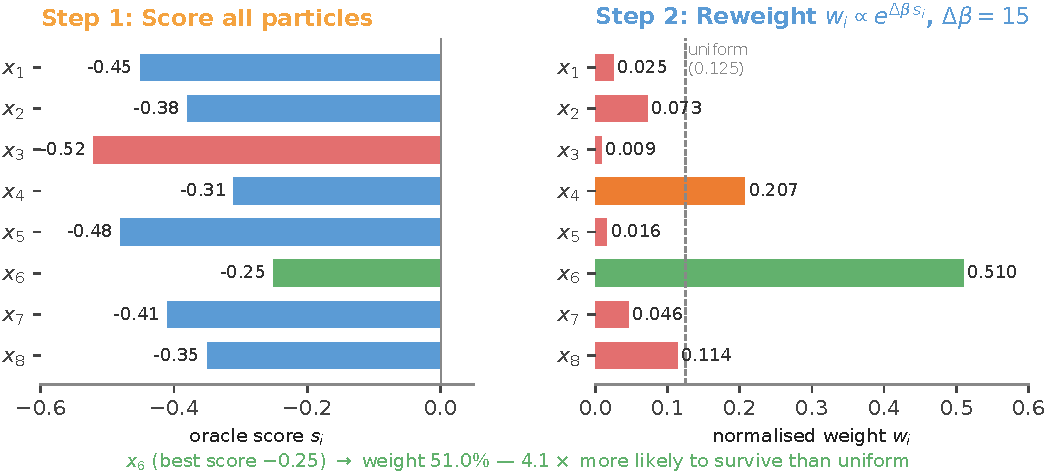
\includegraphics[width=0.95\linewidth]{figures/fig_gpa_walkthrough_score.pdf}
\caption{Score and reweight on the $N\!=\!8$ toy. \textbf{Left:} per-particle oracle scores $s_i$ (best in green: $x_6\!=\!-0.25$; worst in red: $x_3\!=\!-0.52$). \textbf{Right:} normalised weights after the tilt $w_i\!\propto\!\exp(\Delta\beta\,s_i)$ at $\Delta\beta\!=\!15$; uniform $1/N\!=\!0.125$ shown dashed. $x_6$ collects $51.0\%$ of the mass---$4.1\!\times$ the uniform expectation.}
\label{fig:walkthrough-score}
\end{figure}

\subsection{Adapting $\Delta\beta$ via bisection on $\ESS$}

The ESS-adaptive schedule (Lemma~\ref{lem:ess}) chooses $\Delta\beta_t$ so that $\ESS\!\geq\!\alpha N$ \emph{exactly} (not below). With $\alpha\!=\!0.5$, the target is $\ESS_{\rm target}\!=\!4$. Algorithm~\ref{alg:bisect} runs 64 bisection iterations on $[\Delta\beta_{\min}, \Delta\beta_{\max}]\!=\![0,1000]$.

\begin{algorithm}[h]
\caption{Bisection for $\Delta\beta$ given $\ESS$ target}\label{alg:bisect}
\begin{algorithmic}[1]
\State \textbf{Input:} scores $\{r_i\}_{i=1}^N$, target $\tau N$, range $[\Delta\beta_{\min}, \Delta\beta_{\max}]$, max iters $T_{\rm bs}$
\For{$t\!=\!1,\dots,T_{\rm bs}$}
    \State $\Delta\beta_{\rm mid}\!\leftarrow\!(\Delta\beta_{\min}+\Delta\beta_{\max})/2$
    \State $w_i\!\leftarrow\!\exp(\Delta\beta_{\rm mid}\,r_i)/Z$, with $Z\!=\!\sum_j\exp(\Delta\beta_{\rm mid}\,r_j)$
    \State $\ESS\!\leftarrow\!1/\sum_i w_i^2$
    \If{$\ESS > \tau N$} $\Delta\beta_{\min}\!\leftarrow\!\Delta\beta_{\rm mid}$ \Comment{can push harder}
    \Else \;$\Delta\beta_{\max}\!\leftarrow\!\Delta\beta_{\rm mid}$ \Comment{too aggressive}
    \EndIf
\EndFor
\State \textbf{Return:} $\Delta\beta_{\min}$
\end{algorithmic}
\end{algorithm}

For our example, the bisection converges to $\Delta\beta\!\approx\!11.7$, giving $\ESS\!\approx\!4.0\!=\!\alpha N$. The hand-picked $\Delta\beta\!=\!15$ above (which produced $\ESS\!=\!3.08$) was therefore more aggressive than the auto-schedule would choose.

\begin{figure}[h]
\centering
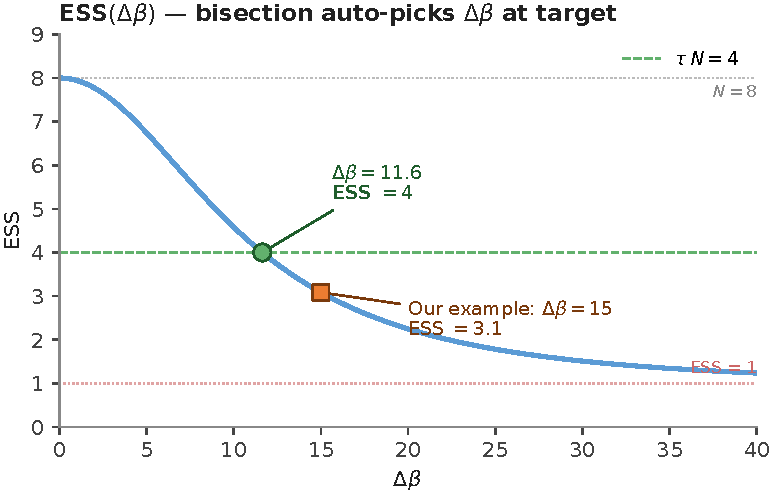
\includegraphics[width=0.78\linewidth]{figures/fig_gpa_walkthrough_ess.pdf}
\caption{$\ESS(\Delta\beta)$ for the $N\!=\!8$ toy oracle scores. The function decreases monotonically from $\ESS\!=\!N$ at $\Delta\beta\!=\!0$ toward $\ESS\!=\!1$ as $\Delta\beta\!\to\!\infty$ (winner-take-all). Bisection finds the unique $\Delta\beta\!=\!11.7$ at which $\ESS$ hits the target $\tau N\!=\!4$ (green dot). The hand-picked $\Delta\beta\!=\!15$ used in the walk-through (orange square) is past the target and so over-collapses the population.}
\label{fig:walkthrough-ess}
\end{figure}

\subsection{Resampling: multinomial vs.\ systematic}

\paragraph{Multinomial.} Draw counts $\!=\!(c_1,\dots,c_N)\!\sim\!\mathrm{Multinomial}(N, w)$. Expected copies per particle are $\E[c_i]\!=\!N\!\cdot\!w_i$, but the realised counts are noisy.

\paragraph{Systematic.} Lay the weights end-to-end as a unit interval $[0,1]$ (segment $i$ has width $w_i$). Drop $N$ pointers at positions $u\!+\!k/N$ for $k\!=\!0,\dots,N\!-\!1$, with $u\!\sim\!\mathrm{Uniform}[0,1/N)$. Particle $i$ receives a number of copies equal to the count of pointers in its segment. This has identical mean to multinomial but lower variance, and is the default in \gpa{}.

For our $N\!=\!8$ example with $u\!=\!0$, the eight pointers at $\{0.000, 0.125, 0.250, 0.375, 0.500, 0.625, 0.750, 0.875\}$ land in segments as follows: $w_2$ (cumulative 0.025--0.098) captures pointer 0.097; $w_4$ (0.107--0.314) captures pointers at 0.125, 0.250; $w_6$ (0.330--0.840) captures pointers at 0.375, 0.500, 0.625, 0.750; $w_8$ (0.886--1.000) captures pointer 0.875. Final copy counts:
\begin{center}
\begin{tabular}{lcccccccc}
\toprule
$i$       & 1 & 2 & 3 & 4 & 5 & 6 & 7 & 8 \\
copies    & 0 & 1 & 0 & 2 & 0 & 4 & 0 & 1 \\
\bottomrule
\end{tabular}
\end{center}
Four particles ($x^1, x^3, x^5, x^7$) are eliminated; $x^6$ is duplicated four times. After resampling, weights reset to $1/N\!=\!0.125$ uniformly.

\begin{figure}[h]
\centering
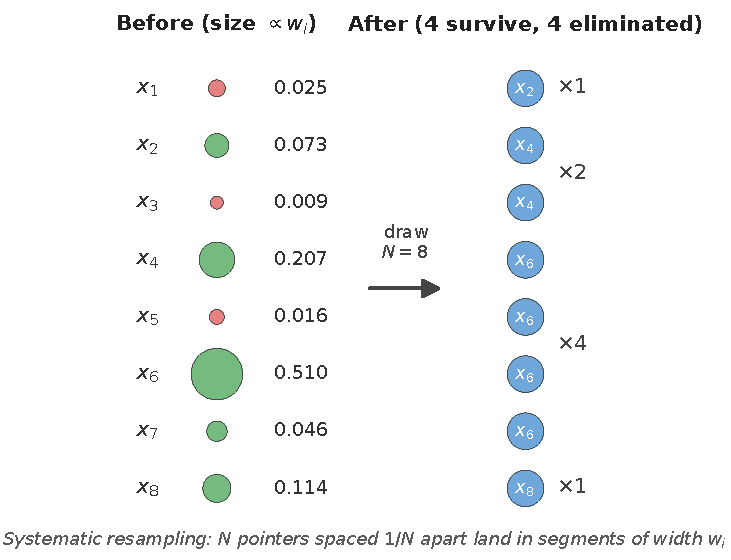
\includegraphics[width=0.85\linewidth]{figures/fig_gpa_walkthrough_resample.pdf}
\caption{Systematic resampling of the $N\!=\!8$ toy. \textbf{Left:} bubble area is proportional to $w_i$; green = retained, red = eliminated by the resampling step. \textbf{Right:} after resampling, all weights reset to $1/N$; $x_6$ now appears four times, $x_4$ twice, $x_2$ and $x_8$ once each. Four particles ($x_1, x_3, x_5, x_7$) are eliminated.}
\label{fig:walkthrough-resample}
\end{figure}

\subsection{Mutation: partial mask + denoise on a length-12 DNA toy}

Each of the eight resampled (now duplicate-rich) particles is independently mutated by $K_\beta$. Concretely, with mask fraction $\mathrm{nf}\!=\!0.25$ ($\!\to\!\lceil 0.25\!\cdot\!12\rceil\!=\!3$ positions on a length-12 sequence):
\begin{center}
\begin{tabular}{ll}
\toprule
\textbf{Step}        & \textbf{Sequence} \\
\midrule
Before (a duplicate of $x^6$)   & \texttt{ACGTATGCACGT} \\
Random mask 3 positions          & \texttt{AC?TA?GC?CGT} \\
Denoise via $p_\theta$           & \texttt{AC\textbf{T}TA\textbf{A}GC\textbf{A}CGT} \\
\midrule
Net edits                         & pos 3: G$\to$T; \, pos 6: T$\to$A; \, pos 9: C$\to$A \\
\bottomrule
\end{tabular}
\end{center}
Two properties this kernel inherits from the pretrained $p_\theta$:
\begin{itemize}
\item \emph{Grammar preservation.} The denoiser sees the unmasked context and proposes tokens consistent with whatever motif/composition rules $p_\theta$ has learned. Random per-position resampling would not.
\item \emph{Diversity restoration.} The four duplicates of $x^6$ each get an \emph{independent} random mask + denoising pass, so they diverge into four distinct child sequences. Without mutation the population would collapse to four identical copies.
\end{itemize}
The mask fraction $\mathrm{nf}$ controls exploration: $\mathrm{nf}\!=\!0.05$ is local search ($\sim\!10$ positions per step on a 200-bp DNA enhancer), $\mathrm{nf}\!=\!0.20$ is large jumps. Section~\ref{sec:results:ablation} reports sensitivity in the practical range.

%-----------------------------------------------------------------------
\section{Hyperparameters}\label{app:hyper}

Table~\ref{tab:hyper-rerd} lists hyperparameters for the SMC-protocol comparison (\drakes{} eval pair); Table~\ref{tab:hyper-ctrldna} lists those for \ctrldna{} comparison (HyenaDNA + gReLU MSE oracles); Table~\ref{tab:hyper-dnacraft} for \dnacraft{} comparison (HyenaDNA/DiMamba + Enformer 50/50). Default values are bolded.

\begin{table}[h]
\caption{Hyperparameters for the SMC-protocol comparison (HepG2 enhancer, MDLM backbone, \drakes{} split-oracle).}
\label{tab:hyper-rerd}
\centering
\small
\begin{tabular}{lll}
\toprule
Parameter & Mean recipe & Spec recipe \\
\midrule
$N$ (population) & 5000 & 5000 \\
$\alpha$ (ESS threshold) & 0.5 & 0.5 \\
$\beta_*$ (target inverse temp) & 200 & 100 \\
$T_{\max}$ (max steps) & 30, hard cap 200 & 30, hard cap 200 \\
nf (mask fraction) & 0.05 & 0.05 \\
DPS gradient strength $\eta$ & 3000 & 3000 \\
$\mathrm{pw}$ (off-target penalty) & 0 & 0.35 \\
GC bio-filter & [0.45, 0.55] & [0.45, 0.55] \\
\bottomrule
\end{tabular}
\end{table}

\begin{table}[h]
\caption{Hyperparameters for \ctrldna{} comparison (Reddy promoters, HyenaDNA backbone, gReLU MSE oracles, universal recipe).}
\label{tab:hyper-ctrldna}
\centering
\small
\begin{tabular}{ll}
\toprule
Parameter & Universal recipe \\
\midrule
$N$ (population) & 10000 \\
$\alpha$ (ESS threshold) & 0.5 \\
$\beta_*$ & 100 \\
$T_{\max}$ (steps) & 60 \\
nf (mask fraction) & 0.05 \\
$K$ (branch factor) & 8 \\
$\mathrm{pw}$ & 0.35 \\
diversity $\lambda$ (conformity) & \textbf{1.0} \\
DPS & off \\
GC bio-filter & off \\
\bottomrule
\end{tabular}
\end{table}

\begin{table}[h]
\caption{Hyperparameters for \dnacraft{} comparison (Gosai 50/50 split, top-128 by MinGap-Eval). C1 = no GC penalty; C3 = soft GC penalty (gct=0.60), no hard bio-filter.}
\label{tab:hyper-dnacraft}
\centering
\small
\begin{tabular}{lll}
\toprule
Parameter & C1 & C3 \\
\midrule
$N$ (population) & 5000 & 5000 \\
$\beta_*$ & 25 & 25 \\
$\mathrm{pw}$ & 0.30 & 0.30 \\
DPS & on & on \\
GC penalty (gct) & --- & 0.60 \\
GC bio-filter & off & off \\
$K$ & 8 & 8 \\
\bottomrule
\end{tabular}
\end{table}

%-----------------------------------------------------------------------
\section{Full GPA-vs-ISM/LEDIDI tables}\label{app:ism_full}

Single-sequence comparison: GPA row = the one sequence in each pool that maximises $\mathrm{AG}-\mathrm{LN}$ (sweet spot: low LN, high held-out AG). Directly comparable to \ism{}/\ledidi{} which are inherently single-sequence.

\begin{table}[h]
\caption{Single-sequence comparison, K562 enhancer, two seeds (uid=181692 natural, uid=50178 random). \gpa{} row = argmax of $\mathrm{AG}-\mathrm{LN}$ within the 5{,}000-seq pool.}
\label{tab:ism_singleseq}
\centering
\small
\begin{tabular}{llrrr}
\toprule
Seed & Method & Edits & LN & AG \\
\midrule
\multirow{4}{*}{uid=181692}
 & \gpa{} (no DPS) uncap   &  96 & 4.97 & \textbf{3.33} \\
 & \gpa{} (+DPS) cap30     &  60 & 6.21 & \textbf{3.47} \\
 & \ism{} gen 115          & 115 & 8.74 & 2.83 \\
 & \ledidi{} t15 $\lambda$=0.05 & 125 & 9.81 & $-$0.22 \\
\midrule
\multirow{4}{*}{uid=50178}
 & \gpa{} (no DPS) cap30   &  60 & 4.71 & 2.75 \\
 & \gpa{} (+DPS) cap30     &  59 & 6.58 & \textbf{3.61} \\
 & \ism{} gen 115          & 115 & 9.58 & 2.92 \\
 & \ledidi{} t15 $\lambda$=0.05 & 105 &11.66 & $-$0.62 \\
\bottomrule
\end{tabular}
\end{table}

\paragraph{Reading the table.}
A single \gpa{} sequence (e.g.\ +DPS cap30 on uid=50178: LN $6.58$, AG $3.61$) beats \ism{} gen 115 on the held-out AG by $+0.69$ at LN $\sim\!3.0$ lower—better held-out activity \emph{and} less reward-hacking. Under any selection rule, \ledidi{} stays AG-negative; not one of its 50 reruns produces an AG-positive sequence.

\paragraph{Apples-to-apples runtime (single H100, K562 enhancer, 5{,}000-sequence pool).}
Table~\ref{tab:ism_runtime} reports wall-time at matched output volume, averaged across the random and natural pools. \gpa{} is fully population-parallel: a single SMC step propagates all 5{,}000 particles together through the diffusion proposal, so the per-particle cost is the GPU-memory chunk \texttt{mutation\_batch\_size=128} amortised over the population. \ism{} is also nominally population-parallel (5{,}000 independent greedy trajectories), but its sequential cost is fixed at 115 generations per seed, and that dominates wall regardless of how memory chunks are batched. \ledidi{} is chunked-sequential by design: 5{,}000 seeds processed in 39 chunks of 128 along the Gumbel-softmax optimisation. The result is $\sim\!9.3\times$ speedup over \ism{} and $\sim\!3.4\times$ speedup over \ledidi{} at identical pool size and identical hardware.

\begin{table}[h]
\caption{Apples-to-apples runtime: single H100, 5{,}000-sequence K562-enhancer pool, averaged across random and natural seed pools. \gpa{} = v3 noDPS recipe (matches Sec.~\ref{sec:results:ism}). Speedup column is $\mathrm{wall}_{\text{baseline}}/\mathrm{wall}_{\gpa{}}$.}
\label{tab:ism_runtime}
\centering
\small
\begin{tabular}{lllr}
\toprule
Method & Wall (5K pool) & Parallelism & Speedup vs.\ \gpa{} \\
\midrule
\textbf{\gpa{}} & \textbf{$\sim\!11.6$ min} & population-parallel (5{,}000 SMC particles) & --- \\
\ledidi{}       & $\sim\!40$ min     & chunked-sequential (39 chunks $\times$ 128 seeds) & $\sim\!3.4\times$ slower \\
\ism{}          & $\sim\!107.5$ min  & population-parallel, but 115 sequential greedy gens & $\sim\!9.3\times$ slower \\
\bottomrule
\end{tabular}
\end{table}

%-----------------------------------------------------------------------
\section{Full DNA-CRAFT tables (GPA-C1 vs GPA-C3)}\label{app:dnacraft_full}

The headline column in Table~\ref{tab:dnacraft} uses GPA-C3 (\texttt{dps\_pw030\_b25\_gct060\_nobio}). This appendix shows the same benchmark with the alternate recipe variant GPA-C1 (\texttt{dps\_pw030\_b25}, no GC penalty), under the matched-output-budget protocol of Table~\ref{tab:dnacraft} (\texttt{by\_pool\_composite} top-64 from \texttt{gpa\_output\_best\_eval.h5}, 3 reps for both variants). Both variants run at $\sim\!3.6$ min/seed (no MCTS) on the MDLM backbone; the only difference is the soft GC-centering term added to C3's DPS gradient.

\paragraph{Recipe decomposition.}
Each token in the recipe name maps to a specific knob in the GPA algorithm of \S\ref{sec:method}, with no other differences between the two variants:
\begin{itemize}
\item \texttt{dps} -- enables the Gumbel-softmax oracle gradient with strength $\eta\!=\!3000$ (\S\ref{sec:method:ext}, ``Gumbel-softmax oracle gradient (DPS)''). This is a biased proposal in the sense of \S\ref{sec:method:ext} and is shared by both C1 and C3, so the C1$\leftrightarrow$C3 contrast does not move along the DPS-bias axis.
\item \texttt{pw030} -- sets the off-target weight $\mathrm{pw}\!=\!0.30$ in the linear fitness of Eq.~\ref{eq:fitness} (\S\ref{sec:method:pw}); the same $0.30$ weights the off-target term inside the DPS gradient as well.
\item \texttt{b25} -- sets the SMC tilt ceiling $\beta_*\!=\!25$. This is below the default range $\beta_*\!\in\!\{100,200\}$ in \S\ref{sec:exp} and is a deliberately gentler tilt that preserves population diversity at some cost in MinGap; both variants share it.
\item \texttt{gct060} \emph{(C3 only)} -- adds a quadratic centering term $-w\,(g(x)-0.60)^2$ to the DPS objective before backpropagation, where $g(x)\!=\!\overline{P(C)+P(G)}$ is the per-position soft-onehot GC fraction and $w\!=\!10$. The penalty rides inside the same Gumbel-softmax gradient that DPS already computes; it is \emph{not} a hard accept/reject filter.
\item \texttt{nobio} -- disables the hard bio-filter (no \texttt{gc\_low}/\texttt{gc\_high} interval gating). All GC discipline in C3 therefore comes from the soft \texttt{gct060} term in the DPS gradient.
\end{itemize}
Both variants additionally use the default branch factor $K\!=\!8$ (\S\ref{sec:method:ext}, Prop.~\ref{prop:K}) and population $N\!=\!5{,}000$ (Table~\ref{tab:dnacraft} caption), so both target $\pi_{\beta_*}^{(K=8)}\!\neq\!\pi_{\beta_*}$ in the sense of Prop.~\ref{prop:K}; the C1$\leftrightarrow$C3 contrast isolates the GC-centering term with $K$, $\beta_*$, $\mathrm{pw}$, $N$, and the DPS bias all held constant.

\begin{table}[h]
\caption{\dnacraft{} benchmark with the GPA-C1 alternate recipe (\texttt{dps\_pw030\_b25}; no GC penalty), reported alongside the headline GPA-C3 (Table~\ref{tab:dnacraft}). Both columns: \texttt{by\_pool\_composite} top-64 from \texttt{gpa\_output\_best\_eval.h5}, mean (std) over 3 reps. Baselines verbatim from \citet{dnacraft2026}.}
\label{tab:dnacraft_full_eval}
\centering
\scriptsize
\begin{tabular}{llcccccccccc}
\toprule
Cell & Metric & SMC & CG & TDS & DRAKES & D3 & Ledidi & Ctrl-DNA & DNA-CRAFT & \gpa{}-C1 & \gpa{}-C3 \\
\midrule
\multirow{4}{*}{HepG2}
 & MinGap   & 1.61 & $-$0.23 & 0.40 & $-$1.40 & 0.05 & 5.77 & \textbf{7.79} & 4.35 & 6.87 & 6.91 \\
 & Motif    & 0.55 & 0.86 & 0.40 & 0.06 & 0.87 & 0.58 & 0.63 & \textbf{0.92} & 0.90 & \textbf{0.92} \\
 & 3-mer    & 0.81 & 0.97 & 0.74 & $-$0.36 & \textbf{0.98} & 0.76 & 0.49 & \textbf{0.98} & 0.95 & 0.95 \\
 & Diversity& 0.83 & \textbf{1.98} & 0.96 & 1.86 & \textbf{1.98} & \textbf{1.98} & 1.90 & \textbf{1.98} & 1.81 & 1.86 \\
\midrule
\multirow{4}{*}{K562}
 & MinGap   & 4.12 & 0.00 & 1.62 & $-$0.20 & 0.18 & 7.66 & \textbf{9.07} & 5.69 & 8.18 & 8.13 \\
 & Motif    & 0.45 & 0.85 & 0.51 & 0.14 & 0.86 & 0.65 & 0.63 & 0.93 & 0.93 & \textbf{0.94} \\
 & 3-mer    & 0.66 & 0.94 & 0.65 & $-$0.35 & 0.96 & 0.69 & 0.41 & \textbf{0.98} & 0.92 & 0.95 \\
 & Diversity& 0.31 & \textbf{1.98} & 0.64 & 1.96 & \textbf{1.98} & \textbf{1.98} & 1.90 & \textbf{1.98} & 1.56 & 1.83 \\
\midrule
\multirow{4}{*}{SK-N-SH}
 & MinGap   & 0.56 & $-$0.28 & 0.19 & 0.09 & $-$0.01 & 3.03 & 3.72 & 3.23 & \textbf{5.07} & 4.98 \\
 & Motif    & 0.52 & 0.86 & 0.48 & 0.23 & 0.84 & 0.38 & 0.48 & 0.88 & 0.89 & \textbf{0.92} \\
 & 3-mer    & 0.78 & 0.95 & 0.72 & $-$0.38 & 0.93 & 0.37 & 0.20 & \textbf{0.97} & 0.87 & 0.94 \\
 & Diversity& 1.27 & \textbf{1.98} & 0.92 & 1.83 & 1.97 & \textbf{1.98} & 1.86 & \textbf{1.98} & 1.59 & 1.86 \\
\bottomrule
\end{tabular}
\end{table}

\paragraph{Reading.}
GPA-C1 and GPA-C3 give nearly tied MinGap and Motif Spearman on every cell (within seed std on most rows). C3 wins Motif on HepG2 / K562 / SK-N-SH ($+0.02$/$+0.01$/$+0.03$) and 3-mer on K562 / SK-N-SH ($+0.03$/$+0.07$). The biggest practical difference is Diversity: the soft GC-centering term in C3's DPS gradient recovers $+0.05$ to $+0.27$ Shannon bits over C1 on every cell, lifting C3 above the Ctrl-DNA Diversity floor on all three cells. The mechanism is indirect: by penalising drift away from $g(x)\!=\!0.60$ at every Gumbel-softmax step, the term blunts the oracle's tendency to push particles toward narrow high-GC modes, which in turn keeps the population spread out in sequence space. C1 wins MinGap on K562 / SK-N-SH ($+0.05$/$+0.09$) but loses across the rest. C3 is the headline because the +Diversity / +Motif / +3-mer trade dominates the small MinGap give-back; C1 is reported as an ablation that isolates the GC-penalty's contribution.

\paragraph{Backbone caveat.}
\dnacraft{}'s reported numbers in Table~\ref{tab:dnacraft} are obtained on a Mamba-style discrete-diffusion (DiMamba) backbone whose code and pretrained checkpoints are not publicly available; the same paper also reports DiMamba-vs-MDLM ablations that show DiMamba contributes additional biological-faithfulness gains. Our \gpa{}-C1 / \gpa{}-C3 numbers are obtained on the publicly available MDLM backbone of \citet{sahoo2024mdlm} and should be read as a lower bound on what \gpa{} would achieve at backbone parity, by Remark~\ref{rem:agnostic}.

%-----------------------------------------------------------------------
\section{Wall-time table}\label{app:wall}

\begin{table}[h]
\caption{Wall time per seed and 5-seed totals (HepG2, identical H100 hardware, identical HyenaDNA backbone). Wall time excludes downstream motif scoring.}
\label{tab:wall}
\centering
\small
\begin{tabular}{lrr}
\toprule
Method & Wall/seed (h) & 5-seed total (GPU-h) \\
\midrule
\ctrldna{} R200 (RL fine-tune) & $43.5\pm 0.8$ & $\sim\!218$ \\
\gpa{} v3 (K=8, no diversity)  & $3.97\pm 0.59$ & 19.8 \\
\gpa{} v4 (K=8 + rejuvenation) & $2.17\pm 0.22$ & 10.8 \\
\gpa{} v5 (K=8 + diversity)    & $\mathbf{2.22\pm 0.52}$ & $\mathbf{11.1}$ \\
\bottomrule
\end{tabular}
\end{table}

%-----------------------------------------------------------------------
\section{DPS gradient ablation}\label{app:dps_ablation}

Population annealing alone (no DPS) already beats single-chain refinement baselines; DPS gradient is a multiplicative enhancement.

\begin{table}[h]
\caption{DPS gradient ablation on Gosai HepG2.}
\label{tab:dps_ablation}
\centering
\small
\begin{tabular}{llrrr}
\toprule
Track & Metric & \gpa{}-only & \gpa{}+DPS & $\Delta$(DPS) \\
\midrule
Mean & $H_{\mathrm{eval}}$ & $8.73\pm 0.50$ & $\mathbf{10.06\pm 0.19}$ & $+1.33$ \\
Mean & Spec & 1.58 & 3.06 & $+1.48$ \\
Spec & $H_{\mathrm{eval}}$ & $8.28\pm 0.12$ & $9.35\pm 0.20$ & $+1.07$ \\
Spec & Spec & $6.11\pm 1.45$ & $\mathbf{7.61\pm 0.25}$ & $+1.50$ \\
\bottomrule
\end{tabular}
\end{table}

%-----------------------------------------------------------------------
\section{Naturalness audit}\label{app:naturalness}

\begin{table}[h]
\caption{Naturalness audit (HepG2 top-128). \gpa{} produces bio-plausible sequences by construction; \ctrldna{} reward-hacks to non-biological space.}
\label{tab:nat}
\centering
\small
\begin{tabular}{lrrr}
\toprule
Metric & Real (Gosai) & \gpa{} & \ctrldna{} \\
\midrule
GC mean & 0.44 & 0.41 & 0.45 \\
\textbf{bio\_pass\_rate} & 0.51 & $\mathbf{1.00}$ & $\mathbf{0.05}$ \\
max homopolymer & 5.4 & 5.1 & $\mathbf{20.9}$ \\
$k$=3 Pearson & 1.0 & 0.61 & 0.39 \\
HNF1A enrichment & $0\times$ & $10\,040\times$ & $7\,812\times$ \\
\bottomrule
\end{tabular}
\end{table}

\begin{figure}[h]
\centering
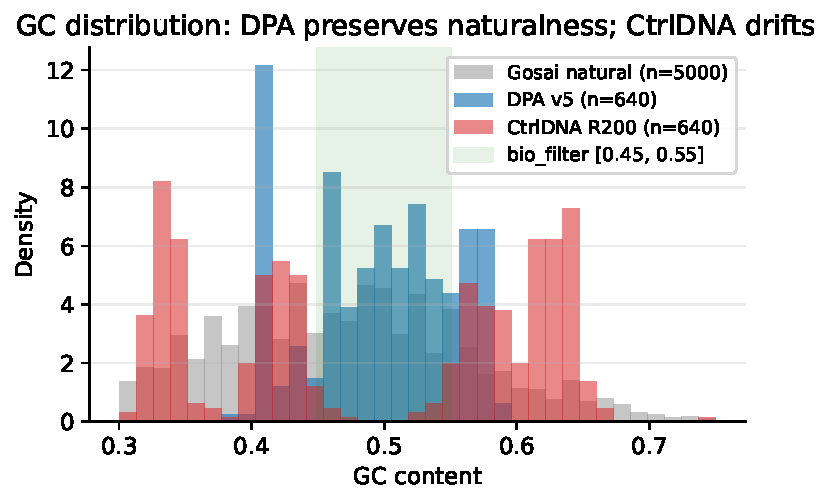
\includegraphics[width=0.6\linewidth]{figures/fig2_gc.pdf}
\caption{GC distribution comparison on HepG2 top-128 sequences. \gpa{} (blue) clusters near the lower edge of the bio-filter (45\%) but stays within the natural Gosai range (gray); \ctrldna{} (red) drifts widely, with a heavy tail of low- and high-GC sequences and a substantial fraction outside the natural distribution.}
\label{fig:gc}
\end{figure}

%-----------------------------------------------------------------------
\section{Extreme specificity}\label{app:extreme}

Pushing $\mathrm{pw}$ beyond the canonical $0.35$ trades $H_{\mathrm{eval}}$ for higher specificity until both off-targets fall below baseline (Table~\ref{tab:extreme}).

\begin{table}[h]
\caption{Extreme-specificity extension on Gosai HepG2 (single run each, $N\!=\!5000$).}
\label{tab:extreme}
\centering
\small
\begin{tabular}{rrrrr}
\toprule
$\mathrm{pw}$ & $H_{\mathrm{eval}}$ & $K_{\mathrm{eval}}$ & $S_{\mathrm{eval}}$ & $H{>}8 \wedge K{<}0 \wedge S{<}0$ \\
\midrule
0.35 & 9.65 & 2.15 &  1.10 & 0 \\
0.50 & 9.54 & 1.96 &  0.63 & 0 \\
0.70 & 8.73 & 1.52 &  0.35 & 0 \\
1.00 & 8.57 & 0.69 & $-$0.48 & 26 \\
1.50 & $\mathbf{8.44}$ & 0.55 & $\mathbf{-0.66}$ & $\mathbf{54}$ \\
\bottomrule
\end{tabular}
\end{table}

\paragraph{Beta trajectory.}
Figure~\ref{fig:beta} shows a representative ESS-adaptive $\beta$ trajectory and the population-mean reward over SMC steps for a HepG2 run.

\begin{figure}[h]
\centering
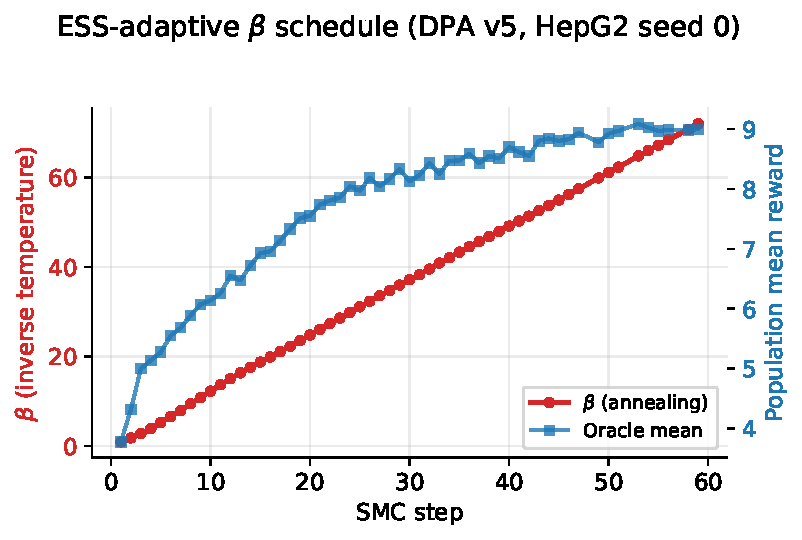
\includegraphics[width=0.6\linewidth]{figures/fig4_beta_traj.pdf}
\caption{Representative \gpa{} run trajectory (HepG2, seed 0). Red trace: ESS-adaptive $\beta$ schedule rises through the annealing path. Blue trace: population mean reward grows monotonically toward saturation as $\beta$ increases.}
\label{fig:beta}
\end{figure}

%-----------------------------------------------------------------------
\section{Negative result: APF correction for $\epsilon$-greedy $K$-branching}\label{app:apf}

A natural attempt to recover Shannon under $K$-branching is to soften the argmax with $\epsilon$-greedy ($\tau\!>\!0$ softmax over the $K$ siblings) and apply the auxiliary-particle-filter weight correction \citep{pittshephard1999}:
\[
w_{\mathrm{new}} = w_{\mathrm{old}}\big/p_\tau(\mathrm{winner}),\qquad p_\tau(j)=\exp(r_j/\tau)\big/\sum_m\exp(r_m/\tau).
\]
Compute the expectation:
\[
\E[w_{\mathrm{new}}\,\varphi(x_{\mathrm{winner}})] = \E_{x_{1:K}\sim q}\!\!\left[\sum_{j=1}^K \frac{\exp(r_j/\tau)}{\sum_m\exp(r_m/\tau)}\cdot\frac{\sum_m\exp(r_m/\tau)}{K\exp(r_j/\tau)}\,\varphi(x_j)\right]=\frac{1}{K}\sum_j \E_q[\varphi(x_j)],
\]
i.e.\ the corrected estimator is equivalent to a single-child sample. The $K$ siblings collapse and the effective-$\beta$ boost vanishes. Empirically, on a synthetic linear reward $r(x)\!=\!3x$ with $q$ uniform on $[0,1]$ (200K Monte-Carlo trials):
\begin{center}
\small
\begin{tabular}{lrrr}
\toprule
Variant & $\E[x]$ & $\mathrm{Var}[x]$ & ESS \\
\midrule
$K=1$ no selection                & 0.5000 & 0.0833 & 100.0\% \\
$K=8$ argmax (no correction)      & 0.8887 & 0.0099 & 100.0\% \\
$K=8$ softmax $\tau\!=\!0.3$ (no corr.) & 0.8445 & 0.0180 & 100.0\% \\
\textbf{$K=8$ softmax $\tau\!=\!0.3$ + APF} & 0.4880 & 0.0874 & 0.4\% \\
$K=8$ softmax $\tau\!=\!1.0$ + APF & 0.5009 & 0.0829 & 53.1\% \\
\bottomrule
\end{tabular}
\end{center}
ESS collapses at low $\tau$ and the corrected mean/variance reproduces $K=1$. We therefore do \emph{not} use APF correction for production runs and report only argmax $K$-branching. K-annealing schedules and waste-free SMC \citep{dau2022wastefree} remain valid theoretical alternatives, deferred to future work.

%-----------------------------------------------------------------------
\section{Negative result: post-hoc Metropolis tempering}\label{app:posthoc}

Another natural Shannon-rescue move is to load the concentrated argmax-$K$ pool and run Metropolis–Hastings at lower $\beta'$ to spread the population. We tested this on the K562 promoter pool (50 MH steps, nf=0.05, HyenaDNA proposal):

\begin{center}
\small
\begin{tabular}{rrrrr}
\toprule
$\beta'$ & accept rate & $\Delta$comp & $\Delta$tgt & $\Delta H$ \\
\midrule
25 &  3.4\% & $+0.02$ & $-0.06$ & $+0.05$ \\
12 &  6.5\% & $-0.15$ & $-0.27$ & $+0.10$ \\
 6 & 13.1\% & $-0.68$ & $-0.77$ & $+0.21$ \\
 3 & 29.1\% & $-2.12$ & $-2.22$ & $+0.39$ \\
 1 & 73.7\% & $-4.71$ & $-5.35$ & $+0.61$ \\
\bottomrule
\end{tabular}
\end{center}
The Pareto slope is $\sim\!3\!-\!5$ target units per $0.1$ nat of Shannon, far too steep for the diversity gap to \dnacraft{}/\ctrldna{} K562 ($\sim\!0.5$ nat) to be closed without erasing the target advantage. Increasing chain length or shrinking nf does not change the local-neighborhood geometry. The honest reading: under sharply peaked oracles, the activity–diversity tension is in the reward landscape, not the sampler.

%-----------------------------------------------------------------------
\section{GC distribution and floor-hugging}\label{app:gc}

Even with the bio-filter $\mathrm{GC}\!\in\![0.45,0.55]$, $60\!-\!75\%$ of \gpa{} top-128 sequences cluster at the lower bound. Two facts:
\begin{enumerate}
\item This is a property of the \emph{masked-diffusion proposal} at low noise fraction. At $\mathrm{nf}\!=\!0.20$ the bias inverts toward the upper bound (GC $\approx\!0.54$); the crossover occurs near $\mathrm{nf}\!\approx\!0.16\!-\!0.17$.
\item The eval oracle is GC-agnostic: at both $\mathrm{nf}$ extremes, top-128 oracle scores are comparable. The GC bias arises from $p_\theta$, not from the reward signal.
\end{enumerate}
Three mitigations were tested with mixed success: (i) GC-aware DPS gradient (\verb|gc_dps_weight|) reduces floor-hugging from $61.5\%$ to $55.0\%$ at $-0.09$ $H_{\mathrm{eval}}$ cost; (ii) narrow $1\%$ GC bands achieve uniform GC by construction at $-0.25$ $H_{\mathrm{eval}}$; (iii) stratified resampling within $2\%$ GC bins \citep{verge2015island} achieves balanced coverage at $-0.50$ to $-1.0$ $H_{\mathrm{eval}}$. We report all three options in the codebase but use the unmitigated baseline in the headline tables for fair comparison with peer methods.

%-----------------------------------------------------------------------
\section{Ctrl-DNA enhancer comparison (V7 main + V5/V8 ablations)}\label{app:ctrldna_enhancer}

This appendix gives the dedicated \ctrldna{}-vs-\gpa{} enhancer comparison referenced in \S\ref{sec:results:promoter}. Same Gosai 50/50 split as the \dnacraft{} benchmark, top-128 selection per cell, 5 \gpa{} seeds. The headline GPA recipe is V7 (universal: $K\!=\!8$, diversity $\lambda\!=\!1.0$); V8a, V8b (alternative pairwise-suppression formulations) and V5 (the previous default with $\lambda\!=\!0.2$) are ablations.

\begin{table}[h]
\caption{Ctrl-DNA vs.\ \gpa{} on Gosai HepG2/K562/SKNSH enhancers (5 seeds; mean (std)). Headline = V7 universal recipe; V8a (log\_ratio + pw=1.0), V8b (linear + pw=1.0) and V5 ($\lambda\!=\!0.2$) are ablations of the diversity / pairwise-suppression knob. \texttt{target\_raw} = mean target oracle score; \texttt{ΔR} = normalised target minus mean off-target; \texttt{shannon} = per-position entropy; \texttt{motif\_corr} = FIMO Pearson against per-cell real reference.}
\label{tab:ctrldna_enhancer}
\centering
\footnotesize
\setlength{\tabcolsep}{4pt}
\begin{tabular}{llrrrr}
\toprule
Cell & Method & target\_raw $\uparrow$ & ΔR $\uparrow$ & shannon $\uparrow$ & motif\_corr $\uparrow$ \\
\midrule
\multirow{5}{*}{HepG2}
 & \ctrldna{} R200             & 5.32 (0.65) & 0.48 (0.10) & 1.65 (0.14) & \textbf{0.29} (0.16) \\
 & \gpa{} V5 ($K\!=\!8, \lambda\!=\!0.2$) & 9.86 (0.10) & 0.85 (0.01) & 1.49 (0.03) & 0.19 (0.03) \\
 & \gpa{} V7 ($K\!=\!8, \lambda\!=\!1.0$) & \textbf{9.90} (0.12) & 0.84 (0.02) & 1.59 (0.11) & 0.20 (0.02) \\
 & \gpa{} V8a (log\_ratio, pw=1.0) & 6.61 (0.04) & 0.68 (0.01) & \textbf{1.93} (0.00) & 0.15 (0.02) \\
 & \gpa{} V8b (linear, pw=1.0) & 9.51 (0.10) & \textbf{0.93} (0.02) & 1.70 (0.11) & 0.10 (0.04) \\
\midrule
\multirow{5}{*}{K562}
 & \ctrldna{} R200             & \textbf{9.99} (1.52) & \textbf{0.77} (0.14) & 1.60 (0.15) & 0.24 (0.07) \\
 & \gpa{} V5 ($K\!=\!8, \lambda\!=\!0.2$) & 8.82 (0.13) & 0.34 (0.00) & 1.43 (0.09) & \textbf{0.26} (0.02) \\
 & \gpa{} V7 ($K\!=\!8, \lambda\!=\!1.0$) & 8.83 (0.12) & 0.32 (0.01) & 1.65 (0.02) & 0.24 (0.02) \\
 & \gpa{} V8a (log\_ratio, pw=1.0) & 6.48 (0.03) & 0.39 (0.01) & \textbf{1.94} (0.01) & 0.24 (0.01) \\
 & \gpa{} V8b (linear, pw=1.0) & 8.15 (0.04) & 0.41 (0.01) & 1.68 (0.02) & 0.25 (0.02) \\
\midrule
\multirow{5}{*}{SK-N-SH}
 & \ctrldna{} R200             & 9.93 (1.13) & \textbf{0.71} (0.10) & 1.63 (0.17) & \textbf{0.23} (0.10) \\
 & \gpa{} V5 ($K\!=\!8, \lambda\!=\!0.2$) & \textbf{14.33} (0.20) & 0.10 (0.01) & 1.49 (0.04) & \textbf{0.23} (0.01) \\
 & \gpa{} V7 ($K\!=\!8, \lambda\!=\!1.0$) & 14.17 (0.18) & 0.10 (0.00) & 1.63 (0.04) & 0.20 (0.01) \\
 & \gpa{} V8a (log\_ratio, pw=1.0) & 6.29 (0.08) & 0.22 (0.01) & \textbf{1.91} (0.01) & 0.15 (0.01) \\
 & \gpa{} V8b (linear, pw=1.0) & 8.26 (0.15) & 0.29 (0.03) & 1.74 (0.05) & 0.10 (0.01) \\
\bottomrule
\end{tabular}
\end{table}

\paragraph{Headlines.}
\gpa{} V7 (the universal recipe) wins target\_raw on HepG2 and SK-N-SH ($+4.58$ and $+4.24$ over \ctrldna{}), and is competitive on K562 within $\sim$1 std. \ctrldna{} retains a ΔR (specificity) edge on K562 and SK-N-SH at the cost of $\sim$50\% lower target activity on HepG2/SK-N-SH and high seed-to-seed variance ($\pm 1.13$--$1.52$). The V7 vs.\ V5 comparison shows the diversity-$\lambda$ bump (from $0.2$ to $1.0$) buys $+0.10$--$0.22$ shannon on every cell at zero target cost, isolating the population-conformity penalty as a strict Pareto improvement. V8a/V8b are alternative pairwise-suppression formulations: V8a (log-ratio reward, pw=1.0) achieves the tightest shannon ($1.91$--$1.94$, near uniform) but at substantial target cost; V8b (linear, pw=1.0) recovers HepG2/K562 target while maximising HepG2 ΔR. The four GPA variants together trace a Pareto front in (target, shannon, motif) space at fixed inference cost---one knob per recipe, no retraining.

%-----------------------------------------------------------------------
\section{DNA-CRAFT $K$ and $i$ scaling sweeps (UCB-MCTS variant)}\label{app:ucb_scaling}

\paragraph{Why MCTS at all.}
DNA-CRAFT replaces the SMC population with a single depth-bounded Monte Carlo Tree Search loop on a DiMamba diffusion backbone, and shows that this delivers state-of-the-art motif and 3-mer grammar fidelity on the Gosai enhancer benchmark (Table~\ref{tab:dnacraft}). The mechanism that delivers their grammar bar is plausible on its face: tree search amortises the cost of choosing the right next mutation by replaying the same scoring oracle across multiple competing children before committing—a strictly more informed proposal than picking the first child that scores well. \gpa{}'s standard $K$-branch is a depth-1 special case of this idea: try $K$ candidates from the proposal and keep the best (Sec.~\ref{sec:method:ext}). It is natural to ask whether the same \emph{deeper} planning that powers \dnacraft{}'s grammar—expanding the best leaves over multiple iterations rather than just one---closes \gpa{}'s residual gap to \dnacraft{} on motif/3-mer correlation. The \texttt{ucb\_stacked} variant exists to test exactly that question.

\paragraph{What \texttt{ucb\_stacked} does, step by step.}
At every SMC mutation step, each particle $x_t^{(j)}$ becomes the root of an independent Monte Carlo tree. We then run $i$ iterations on that tree, where each iteration follows the standard four-phase MCTS-with-UCB1 loop \citep[``UCT'';][]{kocsis2006uct}:
\begin{enumerate}
\item \emph{Selection.} Traverse from the root to a leaf by greedily picking, at each internal node $v$ with already-expanded children $\{a\}$, the child that maximises the UCB1 score \citep{auer2002ucb,kocsis2006uct}
\begin{equation}\label{eq:ucb1}
    \mathrm{UCB1}(a) \;=\; \bar{Q}(a) \;+\; c\sqrt{\frac{\ln n(v)}{n(a)}},
\end{equation}
where $\bar{Q}(a)\!\in\![0,1]$ is the mean (range-normalised) reward backed up through child $a$, $n(a)$ is the visit count of $a$, $n(v)\!=\!\sum_a n(a)$ is the parent visit count, and $c\!=\!\sqrt{2}$ is the standard exploration constant. The first term exploits children with high empirical value; the second term explores low-visit children with a $\sqrt{\log n / n(a)}$ confidence radius. Together this is the canonical bandit rule of \citet{auer2002ucb} for stochastic multi-armed bandits, and \citet{kocsis2006uct} show that applying it node-wise inside a tree (UCT) inherits the same $\mathcal{O}(\log n)$ regret bound at each node. Children with $n(a)\!=\!0$ are tried first by convention so the second term remains well-defined.
\item \emph{Expansion.} Apply \gpa{}'s standard $K$-branch operator at the selected leaf: draw $K\!=\!8$ children using partial-mask$\circ$denoise + DPS (the same operator the no-MCTS \gpa{} would use as its mutation kernel).
\item \emph{Evaluation.} Score each new child under the eval-side reward.
\item \emph{Backpropagation.} Update visit counts $n(\cdot)$ and value estimates $\bar{Q}(\cdot)$ along the path from each new child up to the root, so the next iteration's UCB1 selection (Eq.~\ref{eq:ucb1}) uses fresh statistics.
\end{enumerate}
We bound the tree depth at $d\!=\!2$, so the planner looks at most two mutation steps ahead. After $i$ iterations the tree has at most $1\!+\!i\!\cdot\!K$ nodes; the mutated state for $x_t^{(j)}$ is the highest-reward leaf in that tree. The SMC step then proceeds as usual: the new particle states are importance-weighted at the next $\beta$, resampled if $\ESS$ degenerates, and the loop continues.

\paragraph{Connection to \dnacraft{}.}
The four-step loop (UCB selection $\to$ $K$-fold expansion $\to$ scoring $\to$ reward backprop) is identical in shape to \dnacraft{}'s tree search. What differs is the \emph{scope} of where the tree sits and how it is consumed:
\begin{itemize}
\item \dnacraft{} runs \emph{one} MCTS for the whole design problem: $N_{\mathrm{iter}}\!=\!64$ iterations, $M\!=\!128$ children per expansion, full leaf-to-clean rollouts. Their MinGap-Set archive accumulates the best $N_{\max}\!=\!64$ leaves seen during the run, and that archive is the output (no SMC, no population).
\item \texttt{ucb\_stacked} runs \emph{many} MCTSs: one per particle, per SMC step. Each tree is run for $i\!\in\!\{12,18,24,36\}$ iterations with $K\!=\!8$ children per expansion at depth $d\!=\!2$, no full rollouts (we score after one denoising step). The output is the SMC population at the final $\beta$, exactly as in standard \gpa{}; the trees are only the per-particle mutation kernel.
\end{itemize}
``Stacked'' refers to the layering: MCTS sits \emph{on top of} the $K$-branch+DPS proposal in the SMC inner loop. The $K$-branch supplies the unit of expansion; UCB1+depth-2 lookahead is the planner that decides which leaf is worth expanding next. In effect, \texttt{ucb\_stacked} is a way to ask: does \dnacraft{}'s planning shape, used as a mutation kernel inside SMC, give us the same grammar advantages \dnacraft{} reports as the entire search?

\paragraph{Cost.}
Each \texttt{ucb\_stacked} mutation step performs $1\!+\!i\!\cdot\!K$ scoring calls per particle (vs.\ standard \gpa{}'s 8). At our default $K\!=\!8, i\!=\!18$ this is $145$ scoring calls per particle per step---roughly $18\!\times$ the standard \gpa{} mutation budget. The wallclock overhead is sub-linear in both axes (we report the empirical scaling laws below); for the $i\!=\!18$ headline configuration this works out to $\sim\!7\!\times$ the standard \gpa{}-C3 wallclock per seed.

\paragraph{What the tables below show.}
The two sweeps below sit on K562 and fix one axis at the pilot value while sweeping the other ($K\!=\!8$ for the $i$-sweep, $i\!=\!12$ for the $K$-sweep), at depth $d\!=\!2$ throughout. Wallclock is per seed on a single H100; all metrics are reported under the matched-output-budget protocol of Table~\ref{tab:dnacraft} (\texttt{by\_pool\_composite} top-64 from \texttt{gpa\_output\_best\_eval.h5}). Both sweeps include the standard $K\!=\!8, i\!=\!12$ pilot anchor (5 seeds) for cross-reference.

\begin{table}[h]
\caption{DNA-CRAFT $i$-axis sweep (K562, $K\!=\!8$, $d\!=\!2$). \texttt{by\_pool\_composite} top-64. 5 seeds for $i\!\in\!\{12,18\}$, 2 seeds for $i\!\in\!\{24,36\}$.}
\label{tab:ucb_i_sweep}
\centering
\small
\begin{tabular}{rrrrrrr}
\toprule
$i$ & $n$ & wall (min) & MinGap & Motif & 3-mer & Diversity \\
\midrule
12 & 5 & 31.35 (3.62) & $+$8.066 (0.063) & 0.940 (0.004) & 0.945 (0.023) & 1.903 (0.022) \\
18 & 5 & 32.26 (0.62) & $+$8.115 (0.013) & 0.942 (0.003) & 0.961 (0.003) & 1.926 (0.027) \\
24 & 2 & 37.07 (4.08) & $+$8.153 (0.075) & 0.940 (0.002) & 0.968 (0.003) & 1.941 (0.012) \\
36 & 2 & 46.60 (3.23) & $+$8.015 (0.001) & 0.941 (0.003) & 0.965 (0.002) & 1.937 (0.014) \\
\bottomrule
\end{tabular}
\end{table}

\begin{table}[h]
\caption{DNA-CRAFT $K$-axis sweep (K562, $i\!=\!12$, $d\!=\!2$). \texttt{by\_pool\_composite} top-64. 5 seeds for $K\!=\!8$ (pilot anchor), 2 seeds for $K\!\in\!\{16,24,32\}$.}
\label{tab:ucb_K_sweep}
\centering
\small
\begin{tabular}{rrrrrrr}
\toprule
$K$ & $n$ & wall (min) & MinGap & Motif & 3-mer & Diversity \\
\midrule
 8 & 5 & 31.35 (3.62) & $+$8.066 (0.063) & 0.940 (0.004) & 0.945 (0.023) & 1.903 (0.022) \\
16 & 2 & 49.39 (6.64) & $+$8.124 (0.108) & 0.939 (0.002) & 0.959 (0.008) & 1.898 (0.043) \\
24 & 2 & 69.00 (13.13) & $+$8.070 (0.016) & 0.942 (0.004) & 0.953 (0.007) & 1.935 (0.008) \\
32 & 2 & 77.40 (4.31) & $+$8.022 (0.103) & 0.936 (0.000) & 0.953 (0.002) & 1.907 (0.045) \\
\bottomrule
\end{tabular}
\end{table}

\paragraph{Reading.}
Wallclock is sub-linear in both axes ($\mathrm{wall}\propto i^{0.369}$, $R^2\!=\!0.91$; $\mathrm{wall}\propto K^{0.672}$, $R^2\!=\!0.99$): MCTS-rollout batching and K-branch parallelisation amortise cost. Under the matched-output-budget pool-composite selection, MinGap is saturated across the full $i$ and $K$ sweeps (range $8.02$--$8.15$, within seed std on every row); Motif and Diversity are also flat ($\Delta < 0.01$ across $i$, $\Delta < 0.04$ across $K$); only 3-mer Pearson shows a mild gain with $i$ ($+0.020$ from $i\!=\!12$ to $i\!=\!24$). UCB-MCTS planning therefore buys negligible additional metric gain over the standard \gpa{}-C3 headline at substantial wallclock overhead, which is why C3 (no MCTS) is the headline column in Table~\ref{tab:dnacraft} and \texttt{ucb\_stacked} is reported here only as an optional variant.

%-----------------------------------------------------------------------
\section{Population-size ($N$) ablation}\label{app:n_sweep}

The headline GPA-C3 numbers in Table~\ref{tab:dnacraft} use the standard $N\!=\!5{,}000$ SMC particle population. SMC theory predicts that the empirical distribution converges to the reward-tilted target at the parametric rate $\mathcal{O}(1/\sqrt{N})$ (Theorem~\ref{thm:smc-app}); the population-as-budget reading in \S\ref{sec:method:smc-recap} predicts \emph{monotonic improvement of every reported metric with growing $N$}. We test this directly: holding the C3 recipe and the matched-output-budget selection rule (\texttt{by\_pool\_composite} top-64) fixed, sweep $N\!\in\!\{128, 500, 1000, 2500, 5000, 10000, 20000\}$ across all three cells of the \dnacraft{} enhancer benchmark, 5 SMC seeds per $(N, \text{cell})$ pair.

\begin{table}[h]
\caption{$N$-axis ablation on the \dnacraft{} enhancer benchmark; GPA-C3 (no MCTS), \texttt{by\_pool\_composite} top-64 from \texttt{gpa\_output\_best\_eval.h5}. Mean (std) over 5 SMC seeds. Every metric improves monotonically with $N$ on every cell, validating the population-as-budget framing of \S\ref{sec:method:smc-recap}.}
\label{tab:n_sweep}
\centering
\small
\begin{tabular}{rrrrr}
\toprule
$N$ & MinGap $\uparrow$ & Motif $\uparrow$ & 3-mer $\uparrow$ & Diversity $\uparrow$ \\
\midrule
\multicolumn{5}{l}{\emph{HepG2}} \\
   128 & 6.052 (0.087) & 0.829 (0.036) & 0.757 (0.084) & 1.415 (0.101) \\
   500 & 6.559 (0.153) & 0.884 (0.022) & 0.843 (0.070) & 1.600 (0.167) \\
 1{,}000 & 6.677 (0.130) & 0.895 (0.008) & 0.923 (0.021) & 1.725 (0.104) \\
 2{,}500 & 6.788 (0.129) & 0.912 (0.005) & 0.938 (0.024) & 1.845 (0.029) \\
 5{,}000 & 6.962 (0.076) & 0.915 (0.006) & 0.952 (0.013) & 1.870 (0.056) \\
10{,}000 & 7.013 (0.189) & 0.920 (0.003) & 0.968 (0.005) & 1.908 (0.014) \\
20{,}000 & \textbf{7.081} (0.149) & \textbf{0.928} (0.006) & \textbf{0.972} (0.004) & \textbf{1.912} (0.020) \\
\midrule
\multicolumn{5}{l}{\emph{K562}} \\
   128 & 7.236 (0.160) & 0.871 (0.012) & 0.774 (0.104) & 1.515 (0.120) \\
   500 & 7.709 (0.175) & 0.915 (0.011) & 0.863 (0.044) & 1.677 (0.129) \\
 1{,}000 & 7.968 (0.083) & 0.933 (0.008) & 0.912 (0.106) & 1.813 (0.070) \\
 2{,}500 & 7.995 (0.082) & 0.939 (0.005) & 0.951 (0.017) & 1.821 (0.065) \\
 5{,}000 & 8.193 (0.086) & 0.942 (0.005) & 0.960 (0.010) & 1.893 (0.042) \\
10{,}000 & 8.230 (0.118) & 0.946 (0.004) & 0.965 (0.007) & 1.919 (0.014) \\
20{,}000 & \textbf{8.313} (0.060) & \textbf{0.952} (0.004) & \textbf{0.977} (0.005) & \textbf{1.936} (0.021) \\
\midrule
\multicolumn{5}{l}{\emph{SK-N-SH}} \\
   128 & 2.230 (0.347) & 0.807 (0.028) & 0.672 (0.081) & 1.384 (0.067) \\
   500 & 4.149 (0.470) & 0.887 (0.011) & 0.844 (0.068) & 1.588 (0.128) \\
 1{,}000 & 4.388 (0.282) & 0.899 (0.009) & 0.901 (0.021) & 1.783 (0.049) \\
 2{,}500 & 4.841 (0.062) & 0.908 (0.010) & 0.923 (0.015) & 1.852 (0.017) \\
 5{,}000 & 4.980 (0.079) & 0.919 (0.004) & 0.937 (0.007) & 1.867 (0.042) \\
10{,}000 & 5.054 (0.077) & 0.918 (0.006) & 0.934 (0.022) & 1.892 (0.028) \\
20{,}000 & \textbf{5.209} (0.037) & \textbf{0.926} (0.003) & \textbf{0.946} (0.011) & \textbf{1.917} (0.028) \\
\bottomrule
\end{tabular}
\end{table}

\paragraph{Reading.}
Every metric is monotone-increasing in $N$ on every cell, validating the SMC convergence framing. The 128$\to$20{,}000 range covers $\sim$2.2 orders of magnitude in particle count and yields large absolute improvements: MinGap $+1.0$ to $+3.0$ across cells, Motif Spearman $+0.08$ to $+0.12$, 3-mer Pearson $+0.20$ to $+0.27$, Shannon $+0.42$ to $+0.53$ bits. The headline $N\!=\!5{,}000$ row sits near the elbow on every metric: at $5{,}000\!\to\!20{,}000$ the marginal gain is small (Motif $+0.013$, 3-mer $+0.020$, MinGap $+0.20$, Shannon $+0.04$ averaged across cells), so the headline represents a near-saturated operating point at $\sim$0.043~sec/design. Larger $N$ keeps paying off but at a diminishing rate, consistent with the parametric-$\sqrt{N}$ slope predicted by Theorem~\ref{thm:smc-app}. All runs use the standard GPA-C3 recipe (\texttt{dps\_pw030\_b25\_gct060\_nobio}; $K\!=\!8$ K-branch; no MCTS) on the MDLM backbone, exactly as Table~\ref{tab:dnacraft}; the only knob varied is the SMC particle count $N$.

%-----------------------------------------------------------------------
\section{Per-cell complete tables}\label{app:full_tables}

CSVs for all completed runs across all recipes for each cell are provided as supplementary code. We refrain from reproducing them here; the headline rows in Tables~\ref{tab:dnacraft},~\ref{tab:promoter} reflect the unified-recipe candidates.


\end{document}
